%TC:envir temp [] 0

%%%%%%%%%%%%%%%%%% USAGE INSTRUCTIONS %%%%%%%%%%%%%%%%%%
% - Compile using LuaLaTeX and biber, unless there is a particular reason not to. Do not use the older LaTex/PDFLaTeX or BibTeX. (The fonts won't work correctly.)
% - Font and the report 'year' must be specified when all \documentclass or the template won't work correctly. (There's no error checking/default cases!)
% - For best performance save images/graphics as PDF files, not as png/jpg/eps. This makes no difference to how images are inserted using \includegraphics.
% - As many further packages as wanted can be loaded. Below are just an example set. Note that template itself loads a number of packages, including hyperref.
% - References are handed using biblatex.
% - Link to the presentation of theses policy: https://documents.manchester.ac.uk/DocuInfo.aspx?DocID=2863



%%%%%%%%%%%%%%%%%% META DATA SETUP %%%%%%%%%%%%%%%%%%
% This is where the document title and author are set. Other details for the title page are set later
% Note that if/when you edit these you may need to 'Recompile from scratch' to get the changes to display in the PDF. (In Overleaf, select the down arrow to the right of the 'Recompile' button)
\begin{filecontents*}{\jobname.xmpdata}
    \Title{COMP30040 Report} 
    \Author{10826115} % should be student number rather than name to help with annoymous marking
    \Language{en-GB}
    \Copyrighted{True}
    % More meta-data fielda can be added here if wanted, see https://ctan.org/pkg/pdfx?lang=en for fields
    \end{filecontents*}
    
    
    %%%%%%%%%%%%%%%%%% DOCUMENT SETUP %%%%%%%%%%%%%%%%%%
    \documentclass{uom_eee_dissertation_casson} 
    
    
    %%%%%%%%%%%%%%%%%% PACKAGES AND COMMANDS %%%%%%%%%%%%%%%%%%
    
    % Packages
    \usepackage{graphicx,psfrag,color} % for postscript graphics files
    \graphicspath{ {./images/} }
    \usepackage{amsmath}               % assumes amsmath package installed
    \allowdisplaybreaks[1]           % allow eqnarrays to break across pages
    \usepackage{amssymb}               % assumes amsmath package installed 
    \usepackage{url}                   % format hyperlinks correctly
    \usepackage{rotating}              % allow portrait figures and tables
    \usepackage{multirow}              % allows merging of rows in tables
    \usepackage{lscape}                % allows pages to be typeset in landscape mode
    \usepackage{tabularx}              % allows fixed width tables
    \usepackage{verbatim}              % enhanced version of built-in verbatim environment
    \usepackage{footnote}              % allows more control over footnote environments
    \usepackage{float}                 % allows H option on floats to force here placement
    \usepackage{booktabs}              % improve table line spacing
    \usepackage{lipsum}                % for adding dummy text here
    \usepackage[base]{babel}           % for proper hypthenation in lipsum sections
    \usepackage{subcaption}            % for multiple sub-figures in a single float
    % Add your packages here
    \usepackage{listings}
    \usepackage{adjustbox}
    \usepackage[bottom]{footmisc}
    \usepackage{longtable}
    
    % Optional: for adding alt-text to images:
    %\usepackage{pdfcomment}            % for alt text for accessibility
    % Then to add images use:
    % \pdftooltip{\includegraphics[width=0.5\textwidth]{image.pdf}}{Alt-text here}
    % This makes the text in the image non-select-able though (assuming it's a vector file)
    
    % Custom commands
    \newcommand{\degree}{\ensuremath{^\circ}}
    \newcommand{\sus}[1]{$^{\mbox{\scriptsize #1}}$} % superscript in text (e.g. 1st)
    \newcommand{\sub}[1]{$_{\mbox{\scriptsize #1}}$} % subscript in text
    \newcommand{\sect}[1]{Section~\ref{#1}}
    \newcommand{\fig}[1]{Fig.~\ref{#1}}
    \newcommand{\tab}[1]{Table~\ref{#1}}
    \newcommand{\equ}[1]{(\ref{#1})}
    \newcommand{\appx}[1]{Appendix~\ref{#1}}
    
    
    
    %%%%%%%%%%%%%%%%%% REFERENCES SETUP %%%%%%%%%%%%%%%%%%
    
    % Setup your references here. Change the reference style here if wanted
    \usepackage[style=ieee,backend=biber,backref=true,hyperref=auto]{biblatex}
    % Note backref=true adds a page number (and hyperlink) to each reference so you can easily go back from the references to the main document. You may prefer backref=false if you need to stick strictly to a given reference style
    
    
    % Fixes which can't be applied in the .cls file
    \DefineBibliographyStrings{english}{backrefpage = {cited on p\adddot},  backrefpages = {cited on pp\adddot}}
    %  \renewcommand*{\bibfont}{\large}
    
    
    % Add more .bib files here if wanted
    \addbibresource{references.bib}
    
    
    
    %%%%%%%%%%%%%%%%%% CUSTOM MODIFICATIONS %%%%%%%%%%%%%%%%%%
    \usepackage{xcolor}
    % Define a custom quote environment
    \renewenvironment{quote}
    {
        \par\setlength{\leftskip}{10pt}
        \begin{tabular}{|p{0.9\linewidth}}  % Vertical bar on the left
        \setlength{\leftskip}{10pt}
        \itshape
    }
    {
        \end{tabular}
        \par
    }
    
    % Define a custom temp environment for placeholders, etc.
    \newenvironment{temp}
    {
        \color{red}  % Set text color to red
        \itshape     % Italicize text for further distinction (optional)
    }
    {
        \normalcolor % Reset text color
    }
    
    %%%%%%%%%%%%%%%%%% START DOCUMENT %%%%%%%%%%%%%%%%%%
    
    % Don't edit these lines, title and author are automatically taken from the document meta-data defined above
    \begin{document}
    \makeatletter
    \title{\xmp@Title}
    \studentid{\xmp@Author}
    \makeatother
    
    % Set the below yourself
    \course{Computer Science}  % "Master of Science in" is added automatically
                                                     % Our courses are: Advanced Control and Systems Engineering, Advanced Control and Systems Engineering with Extended Research, Communications and Signal Processing, Communications and Signal Processing with Extended Research, Electrical Power Systems Engineering, Advanced Electrical Power Systems Engineering, Renewable Energy and Clean Technology, Renewable Energy and Clean Technology with Extended Research
    \submitdate{2025}                                  % regulations ask only for the year, not month
    \wordcount{TODO}		                           % use \wordcount{} to set the count, \thewordcount to print in the text
    
    %TC:ignore
    \maketitle
    
    
    %%%%%%%%%%%%%%%%%% LISTS OF CONTENT %%%%%%%%%%%%%%%%%%
    \uomtoc
    % other lists are not required, but can include \uomlof and \uomlot if really want to
    \uomlof
    \uomlot
    
    %%%%%%%%%%%%%%%%%% ABBREVIATIONS %%%%%%%%%%%%%%%%%%%%%
    \phantomsection\addcontentsline{toc}{section}{Abbreviations and Acronyms}
    \section*{Abbreviations and Acronyms}
      % ALWAYS define abbreviations on first use
    
      \begin{description}
        \item[AI] Artificial Intelligence
        \item[API] Application Programming Interface
        \item[CD] Compact Disc
        \item[CDPA] Copyright, Designs and Patents Act 1988
        \item[CLK] Clock (regular pulses used for quadrature rotary encoding)
        \item[CNN] Convolutional Neural Network
        \item[CV] Computer Vision
        \item[DT] Data (offset pulses used for quadrature rotary encoding)
        \item[EN] Enable
        \item[GDPR] General Data Protection Regulation
        \item[GPIO] General-Purpose Input/Output
        \item[GPU] Graphical Processing Unit
        \item[ML] Machine Learning
        \item[OCR] Optical Character Recognition
        \item[OS] Operating System
        \item[PWM] Pulse-Width Modulation
        \item[REST] Representational State Transfer
        \item[RPi] Raspberry Pi
        \item[RPiOS] Raspberry Pi OS (formerly Raspbian)
        \item[RPM] Rotations per Minute
        \item[SBC] Single-Board Computer
        \item[SDK] Software Development Kit
        \item[SRP] Single Responsibility Principle
        \item[SSE] Server-Sent Events
        \item[SW] Switch (the live connection of a button circuit) 
        \item[ToS] Terms of Service
        \item[TOU] Terms of Use
        \item[TPU] Tensor Processing Unit 
        \item[URI] Uniform Resource Identifier
        \item[UX] User Experience
      \end{description}
    
    %%%%%%%%%%%%%%%%%% ABSTRACT %%%%%%%%%%%%%%%%%%%%%%%%%%
    \begin{abstract} % put abstract here. Limit is 1 page.
    
        This project develops an innovative solution that merges the physical and digital music experience by enabling vinyl records to be digitally streamed through image recognition. Leveraging machine learning, the system identifies physical album covers and retrieves corresponding audio tracks from Spotify. Built on a Raspberry Pi 5 platform, it provides users the tangible experience of vinyl while offering the convenience of digital playback. The project's objectives include addressing limitations inherent to vinyl, such as equipment fragility and playback inconvenience, and targeting vinyl enthusiasts who value both aesthetics and usability. Experimentation was conducted with various neural network models to optimise recognition accuracy and reliability. Challenges addressed include accurate image recognition, legal and ethical considerations around copyrighted materials, and robust technological integration. Evaluation shows the developed solution effectively enhances the usability and appeal of vinyl collections.
    
    \end{abstract}%
    \clearpage
    
    
    
    %%%%%%%%%%%%%%%%%% DECLARATIONS %%%%%%%%%%%%%%%%%%
    \uomdeclarations % Don't need unless final thesis
    
    
    
    %%%%%%%%%%%%%%%%%% ACKNOWLEDGEMENTS %%%%%%%%%%%%%%%%%%
    \begin{uomacknowledgements}
    I would like to extend my gratitude to the noble mahogany tree, whose sacrifice provided not only the material for a Welsh love spoon -- by which I proposed and became engaged to my beloved fiancée -- but also the offcuts that found purpose in the physical interface of this project. Your contribution to both my personal and academic life has been truly invaluable.
    
    Also, to my close friend Joshua Bond’s dissertation \cite{jdbond}, which I have yet to finish reading - but I am sure it is great.
    \end{uomacknowledgements}
    
    %TC:endignore
    
    %%%%%%%%%%%%%%%%%% SECTION 1 %%%%%%%%%%%%%%%%%%
    \section{Introduction}
    
      % Written by **Sean Bechhofer**: https://studentnet.cs.manchester.ac.uk/ugt/year3/project/projectbookdetails.php?projectid=55259
    
      % Vinyl is back! According to the [NME](https://www.nme.com/news/music/uk-vinyl-sales-2023-reach-highest-level-since-1990-3563676), UK sales of vinyl in 2023 were the highest seen since 1990. Vinyl has always remained popular among niche genres, but we are also seeing mainstream artists like Taylor Swift and Lana Del Ray releasing, and selling large volumes of albums on the format. Vinyl records have also recently been added in to the ONS "Basket of Goods and Services": a carefully selected set of items representative of the goods and services that UK consumers typically spend their money on ([ONS](https://www.ons.gov.uk/news/news/arecordrevivalthatscookingupastormvinylmusicandairfryersspintheirwayintothebasketofgoods)).
    
      % Fans of the format claim better sound reproduction, with a fuller frequency range and a "warmth" lacking in digital formats such as CD. Playing vinyl requires specialist equipment: while the ritual of putting a disc on the turntable and dropping the needle is, for some, part of the experience, it can also be seen as an inconvenience.
    
      % The aim of this project will be to develop an application that supports a blending of the physical and digital worlds. A physical artefact such as an LP is scanned using a camera. The information on the label or cover is then used to identify the release which can be played. This content could be retrieved from a streaming service such as Spotify or Apple Music, an artist site such as Bandcamp [Bandcamp](https://bandcamp.com/), or the user's own personal media library. This would then allow a user to "play" their records without a turntable. Although the audio quality may not match that of vinyl, such an application would appeal to those who like to collect vinyl for its own sake, or who appreciate the larger format artwork that comes with an old school LP. The application could run on a mobile phone or specialist hardware such as a Raspberry Pi equipped with a camera.
      % Example methods that could be used for identification of the release include bar codes, QR codes or OCR acting on label text.
    
      % For a stretch goal, the application could be extended to cover other media: the cassette tape ([Guardian](https://www.theguardian.com/music/2023/apr/20/fun-way-consume-music-why-sales-of-cassette-tapes-soaring)) is also experiencing a come back, although the [eight-track](https://en.wikipedia.org/wiki/8-track_cartridge) is unlikely to be retrieved from the dustbin of history.
      % The project should be considered as challenging. It will require integration of several technologies and some creativity.
    
        \subsection{Background and motivation}
    
           The resurgence of vinyl records presents both an opportunity and a challenge. Despite their renewed popularity, vinyl records require specialised equipment, careful handling, and manual operation, all of which pose practical barriers for modern listeners.
    
            Combining digital and physical media provides an attractive solution to these challenges by merging the tangible appeal of vinyl with the convenience and accessibility of digital music streaming. Such an integration maintains the emotional and tactile connection that many listeners appreciate in physical collections, while offering the ease of digital technologies. Given current consumer interests and technological advancements, this hybrid approach is timely and relevant, making this project particularly worthwhile.
        
        \subsection{Aims and objectives}
    
            This project aims to resolve key limitations of traditional vinyl playback by providing users the ability to digitally stream music by scanning physical album covers. The specific problems addressed include the inconvenience of manual playback, limitations in portability, and difficulties associated with maintaining physical equipment and media.
    
            The full goals, with tangible criterion, for the evaluation of the model are defined in the Requirements Analysis of the Design (\ref{sec:reqany}).
    
            The intended users of this solution are vinyl enthusiasts, collectors, and casual listeners who appreciate vinyl's tangible and aesthetic aspects but desire greater convenience. This project identifies a significant gap in current workflows, where physical vinyl collections remain underutilised due to the inconvenience of traditional playback systems.
        
        \subsection{Scope}
    
            In scope for this project is the development of an application that uses image recognition technology -- such as machine learning and OCR -- to identify vinyl records and retrieve corresponding digital tracks from streaming platforms like Spotify. The solution supports a Raspberry Pi 5-based hardware platform, integrating both physical and digital user interfaces.
    
            Out of scope elements include extensive hardware customisation beyond essential playback functionality, support for every possible streaming service, and creation of original music databases. The focus will specifically be on leveraging Spotify's streaming capabilities -- due to its widespread adoption and available API support -- whilst still maintaining flexibility and the ability to change APIs easily, if desired.
        
        \subsection{Challenges}
    
            The primary challenges anticipated include accurately identifying album artwork using machine learning techniques, managing legal and ethical concerns related to copyrighted album covers, and effectively integrating multiple technologies -- such as hardware components, web APIs, and neural networks -- into a cohesive system. Ensuring the system is user-friendly while remaining technically robust also presents a significant development challenge.
        
        \subsection{Report structure} % ROADMAP
    
            \begin{temp}
                \begin{itemize}
                    \item How does the structure reflect my development process?
                \end{itemize}
            \end{temp}
        
            This report consists of seven chapters:
            \begin{description}
                \item[Chapter 1] introduces the project, its motivations, objectives, and challenges.
                \item[Chapter 2] presents the background and literature review, discussing existing technologies and relevant research informing design choices.
                \item[Chapter 3] details the project's design decisions, system architecture, and chosen technologies.
                \item[Chapter 4] describes the implementation process, outlining how design considerations translated into practical development.
                \item[Chapter 5] presents the outcomes of the implemented solution, showcasing software and hardware artefacts.
                \item[Chapter 6] evaluates the project's effectiveness, usability, and impact, including comparisons to existing systems.
                \item[Chapter 7] summarises conclusions, identifies project limitations, and suggests avenues for future development.
            \end{description}
    
    %%%%%%%%%%%%%%%%%% SECTION 2 %%%%%%%%%%%%%%%%%%
    \section{Background and Literature Review} % LITERATURE REVIEW / BACKGROUND
      % [ ] summary of similar systems
      % [ ] explanations of concepts relied on later
      % [ ] advanatges and disadvantages of approaches
      % [ ] highlight problems I will improve
      % [ ] cite all references
    
      \subsection{Overview of Related Systems}
    
        Whilst the creation of a digitised turntable software is a rather novel idea, it is important to consider where this sits in the existing landscape; to understand important technologies and design decisions used in similar projects, in order to best utilise them.
      
        \subsubsection{Vinyl Systems}
            % Research into questions such as 'why do people like vinyl so much?' and 'why is it making a comeback?'. Traits distilled from this feed into later design choices (I have chosen to make a make a physical artefact with a mahogany base, because physicality and aesthetics are important the people who would potentially use this system).
    
            \begin{quote}
                ``Vinyl is back!'' \cite{bechhofervttspec}
            \end{quote}
            
            In 2023, UK vinyl sales reached their highest level since 1990 \cite{geraghty2023uk_vinyl_sales}, confirming the ongoing ``vinyl revival'' \cite{vinylRevival} (see Figure~\ref{fig:vinyl_sales}). Initially dismissed as a short-term trend when it emerged in 2008-2009, this resurgence has persisted, highlighting a renewed interest in physical music formats. Understanding the motivations behind this revival is crucial for informing design decisions, particularly from a UX perspective, as vinyl collectors constitute a key target audience.
            
            \begin{figure}[htbp]
                \centering
                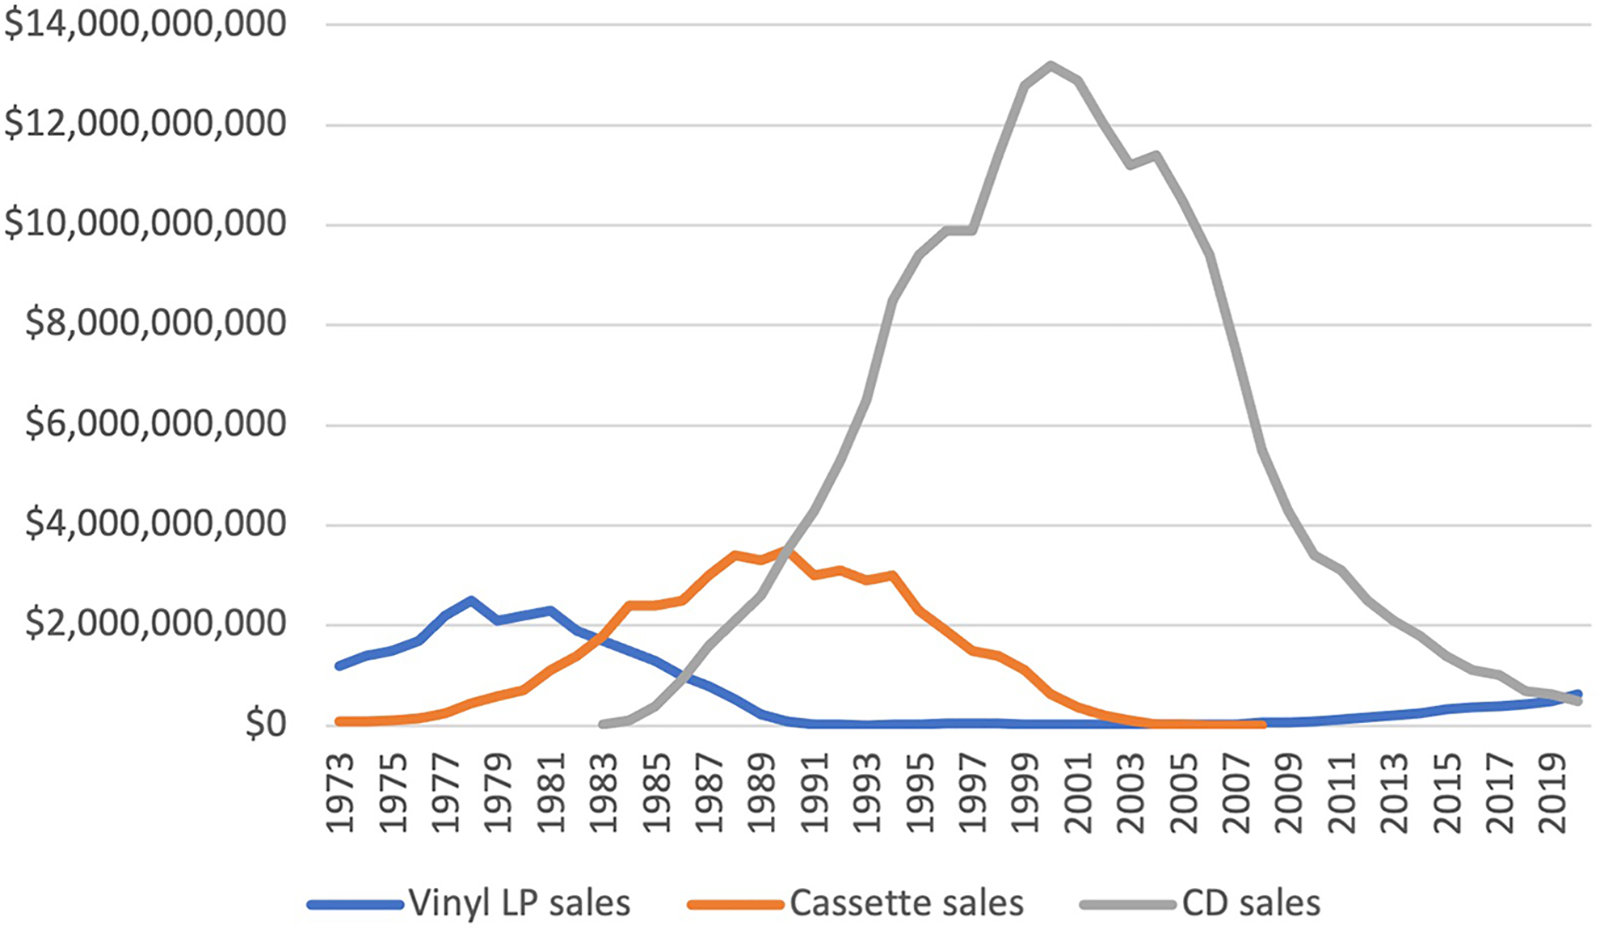
\includegraphics[width=\linewidth]{images/vinyl_sales_2023.png}
                \caption{Vinyl LP, Cassette, and CD Sales Revenue (1973–2020).}
                \caption*{Sourced from Journal of Popular Music Studies \cite{vinylRevival}}
                \label{fig:vinyl_sales}
            \end{figure}
    
            Although now taken for granted, records -- and their predecessors, Edison's cylinders — transformed music from an ephemeral experience into a reproducible medium. Before recording technology, music was transient and confined to its place and time of performance, unable to be stored or shared beyond a live setting. While compositions could be transcribed into musical notation, each unique performance could never be heard again once it ended, unlike with visual art, where many original works from as far back as antiquity still survive \cite{jdbond}.
    
            This revolution in music consumption not only shaped the modern music industry but also cemented vinyl’s cultural significance. By making music ownable and replayable, it changed the way people engaged with it, fostering a more personal and enduring connection. Its enduring appeal, even in the digital age, suggests that its value extends beyond convenience, tapping into a deeper connection with music as a tangible experience.
    
            % Aesthetics
            \paragraph{Aesthetics and Emotional Appeal}
                % nostalgia, vibes
    
                Nostalgia plays a significant role in vinyl's resurgence. Statista data suggests the revival is primarily driven by two age groups: those aged 55+ and 25--34, with other demographics showing less engagement \cite{Gotting2021}. Older generations retain direct sentimental ties to the medium, while younger consumers are drawn to its cultural legacy.
    
                Despite the convenience of digital music, many consumers find it impersonal. In the past, music was a shared experience, often centred around a single household phonograph. Today, listeners frequently engage in isolated listening experiences \cite{historyandrevivalofvinyls}, with it being commonplace for multiple people in the same room to listen to different tracks at the same time. To an extent, music used to demand focus. You could not skip or replay a track without having to carefully reposition the needle. Some seek to reclaim the intentionality of music consumption, preferring a medium that encourages engagement rather than passive background listening \cite{Liu2020}.
    
                To many, music has become hollow- especially as music streaming services have easily monopolised the digital sphere \cite{historyandrevivalofvinyls}. Whether people are  yearning for the experiences of their past, or just a breath of `fresh air', many are turning to vinyl to do so.
    
                People are seeking community around their music and even its medium. Reddit's r/Vinyl, as of 2025, has over 2.2 million members. Whilst vinyl is still a relatively niche option, the social aspect of the internet means that, today, people are not confined to geographical constraints, and so, no matter how niche an interest is, they will be able to find like-minded people to connect to.
          
              % Ownership
              % Physicality
            \paragraph{Physicality and Ownership} % or MATERIALITY; general ethics
    
                Digital media ownership has become increasingly precarious, with consumers often purchasing revocable licenses rather than tangible assets \cite{verge2024steam_license}. This transition has upset many people, with there being many calls to bring back genuine ownership \cite{stanton2024gamers_pushback}, with legislation even being passed in California to make this fact more transparent to consumers \cite{california2024ab2426}.
    
                If a streaming vendor stops serving a particular piece of music, then that album can be lost to the public forever \cite{polygon2024cartoon_network_delisting}. However, if a consumer actually owns the physical discs or digital audio files, then they can ensure that they can listen to their audio, regardless of whatever licensing disputes may lead to the removal of digital media in the future (see \cite{bains2022lotr_strategy}).
    
                Furthermore, there are also concerns that streaming platforms often provide artists with minimal financial compensation, leading some consumers to purchase physical media as a means of direct support \cite{historyandrevivalofvinyls}. This means that there is a demographic of people who both own physical vinyls, but still make use of digital streaming services. Many even purchase physical vinyls despite not owning a device to play them on \cite{Trapp2023}. In addition, the act of gaining a physical good in support of an artist can even result in a psychological feeling of proximity to their idol \cite{historyandrevivalofvinyls}.
                
                Additionally, vinyl's finite nature contrasts with the boundless availability of digital tracks, making collections feel more meaningful and curated.
    
            % Audiophiles
            \paragraph{Audiophilia and Sound Quality}
    
                Another significant factor is the quality of the music being offered.
    
                \begin{quote}
                    \textbf{audiophile}: a person who is especially interested in high-fidelity sound reproduction. \cite{audiophile2025}
                \end{quote}
    
                % quality
                Vinyl is often perceived as superior in audio quality due to early digital compression limitations, such as the distortion issues highlighted in ``Tom's Diner'', wherein the a cappella's clean, isolated vocals revealed artifacts and distortions when encoded in early MP3 formats \cite{TODO}. Modern digital formats generally surpass vinyl in fidelity, particularly in bit depth and dynamic range. However, whilst advances in manufacturing storage drives have somewhat mitigated the need drastically to compress files, there are still valid use cases where extreme compression may be needed, such as for streaming audio on a low-quality network, which may cause the audio to sound worse than on vinyl.
    
                Additionally, as a physical format, vinyls are prone to being scratched and having physical deformities which affect the playback quality. Vinyl enthusiasts appreciate the medium’s imperfections, which are thought to add warmth and character. No two discs sounds exactly the same, whereas digital copies are utterly identical. This also creates a sense of personal ownership with vinyls - not only does the consumer own the physical disc itself, but they own their precise and unique version of it.
    
                It is important to note that many contemporary vinyl releases originate from digital masters, meaning potential losses in fidelity depend on how well an album is adapted to the format. Several inherent limitations affect vinyl playback, including: duration constraints, due to physical disk size; track sequence issues, as resolution gradually degrades towards the inner grooves; and RIAA equalisation, which alters frequency response to accommodate physical limitations of the medium \cite{engineeringvinyls}. Additionally, stereo information handling differs from digital formats, as vinyl relies on lateral and vertical groove modulation, which can introduce crosstalk and phase issues \cite{engineeringvinyls}. These factors, if not carefully managed during production, may compromise the listening experience - meaning modern tracks may often perform better in their original digital forms.
    
            \paragraph{Conclusion}
                While digital audio services offer notable convenience, the enduring vinyl revival demonstrates that many users still value tangible, nostalgic experiences. Nostalgia and charm play a crucial role in this appeal, making it essential to design with these emotional connections in mind. By combining the strengths of both physical and digital formats, a system can provide a richer, more meaningful user experience that aligns with modern consumption habits while preserving the authenticity and personal connection that vinyl enthusiasts cherish. A significant portion of consumers actively engage with both streaming services and physical media, indicating that a hybrid approach has a viable audience.
    
        \subsubsection{Image Recognition}
    
            \begin{temp}
                Y. LeCun and Y. Bengio, 1995, "Convolutional Networks for Images, Speech, and Time-Series". Brain theory neural networks, vol. 3361
            \end{temp}
    
            Image recognition is the creation of software and tools which can be used to identify objects, places, people, etc. in digital images, which has existed since at least 1946 \cite{hall1979computer}. However, in this brief time, the field has undergone several drastic changes as technology has advanced \cite{imagenetclasscnn}, and is still be redefined in the present day, particularly with the arrival of machine learning approaches, with new implementations being utilised across the field (e.g. \cite{RAMPRASAD2025100556}, 2025).
    
            \paragraph{Traditional Methods}
            
                Before the advent of deep learning, image recognition primarily relied on manually crafted feature extraction techniques. Classical methods included edge detection, template matching, and statistical pattern recognition. Notable feature descriptors such as Scale-Invariant Feature Transform (SIFT), Speeded-Up Robust Features (SURF), and Histogram of Oriented Gradients (HOG) played a significant role in object detection and classification \cite{pal2001pattern}. However, these approaches were often limited by their inability to generalise across variations in lighting, scale, and occlusions. The ImageNet Large Scale Visual Recognition Challenge (ILSVRC) served as a benchmark for evaluating the effectiveness of traditional and emerging techniques \cite{russakovsky2015imagenetlargescalevisual}.
            
            \paragraph{Emergence of Convolutional Neural Networks}
            
                The introduction of convolutional neural networks (CNNs) marked a paradigm shift in image recognition. Early work, such as LeNet-5, demonstrated CNNs' potential \cite{726791}, but it was the breakthrough of AlexNet in the 2012 ImageNet competition that solidified their dominance \cite{imagenetclasscnn}. Subsequent architectures, including VGG, ResNet, and EfficientNet, further improved performance by introducing deeper networks, residual connections, and optimised convolutional layers \cite{deppcnnsforimagerecognition}. These advancements enabled significant improvements in tasks such as object detection, facial recognition, and medical image analysis.
    
                In the context of vinyl cover art recognition, CNNs offer a powerful solution for identifying album artwork despite variations in artistic style, degradation, and distortions. However, a key challenge in training CNNs for this task is the limited availability of labelled datasets. Unlike large-scale image classification datasets like ImageNet, curated datasets for album cover recognition remain relatively small. To address this limitation, data augmentation techniques -- such as random cropping, rotation, colour jittering, and synthetic distortions -- help improve model robustness by simulating real-world variations \cite{LIN2025102660}. There has even been research done recently into using stable diffusion techniques to facilitate fully artificial data augmentation, with generative AI \cite{Alimisis2025}.
    
            \paragraph{Multi-Headed Networks and Consensus-Based Recognition}
    
                A limitation of conventional CNN models in image recognition is their reliance on a single decision pathway, which can lead to misclassifications when dealing with visually similar or degraded images. One approach to mitigate this issue is the use of multi-headed neural networks, where multiple CNN branches extract different features and contribute to a consensus decision. This technique allows the network to assess multiple aspects of the image, such as texture, dominant colours, and key object structures, before making a final classification \cite{Zheng2017}. 
            
                By integrating multi-headed architectures with ensemble strategies, models can achieve higher classification accuracy and robustness, particularly when handling ambiguous or visually noisy inputs. This method has been successfully applied in fine-grained classification tasks and could be adapted for vinyl cover recognition by leveraging multiple specialised feature extractors that assess distinct album cover characteristics.
    
            \paragraph{Current 'State of the Art'}
    
                Visual transformers currently represent the state-of-the-art in image classification, significantly outperforming traditional CNNs on large datasets. However, their performance heavily depends on large-scale data availability; with limited or specialised datasets, such as vinyl cover recognition, transformers may perform poorly or be impractical. Thus, CNN-based architectures or hybrid approaches remain more suitable in scenarios with smaller, niche datasets.
    
                A key challenge is ensuring models generalise effectively to unseen data, avoiding overfitting. Techniques like dropout, which randomly deactivate neurons during training, improve robustness by preventing reliance on specific features. Additionally, splitting datasets into training, validation, and test subsets enables monitoring model generalisation, though careful consideration is required to balance partition sizes and representativeness, whilst also avoiding biases. Data augmentation (e.g., rotations, lighting adjustments) further enhances performance by artificially expanding the training data, and improving generalisation by simulating real-world variations. However, larger augmented datasets increase computational demands, making GPU or TPU optimisations essential for efficiency.
    
        \subsection{Legal and Ethical Considerations}
    
          The training and use of machine learning models for image classification requires the acquisition and processing of data, which, in order to effectively handle the cover art of existing albums, necessitates obtaining and using their copyrighted artworks. This raises both legal and ethical concerns, particularly regarding compliance with UK copyright law and exemptions. This section examines the legal basis for dataset usage, fair dealing exemptions, and the ethical implications of using copyrighted material in an academic AI project.
    
              \subsubsection{Copyright Law and Fair Dealing}
                  % explain copyright law
                  Under the \textit{Copyright, Designs and Patents Act 1988} \cite{cdpa1988}, creative works, including album covers, are protected from unauthorised use, reproduction, distribution, and modification.
          
                  % introduce fair dealing
                  However, UK law also provides a key exception known as Fair Dealing, which allows limited use of copyrighted material under specific conditions, although such exemptions are only granted under very specific circumstances and for a very limited scope of use. Importantly, it is not a rigid rule but a context-dependent legal doctrine, evaluated on a case-by-case basis. The law does not explicitly define what qualifies as fair dealing; instead, courts assess whether a use is reasonable and justified based on the combination of several established legal factors.
                  
                  One of the most relevant exemptions is non-commercial research, as outlined in \textit{Section 29(1)} of the CDPA:
                  \begin{quote}
                      Fair dealing with a work for the purposes of research for a non-commercial purpose does not infringe any copyright in the work provided that it is accompanied by a sufficient acknowledgement. \cite{cdpa1988}
                  \end{quote}
    
                  This indicates that non-commercial academic research can be exempt from copyright infringement if proper attribution is provided. However, the applicability of this exemption depends on further and additional factors, such as the amount of material used and its impact on the copyright holder’s market.
    
              % 1. Using a dataset to create a model
              \subsubsection{Use of Artworks in Model Training}
              
                  Album covers are protected by copyright as highly creative works. Any reproduction or modification is typically restricted without permission from the copyright holder. As such, the bar needed for fair dealings is very high when dealing with such artwork. However, training a classification model may qualify for fair dealing, provided certain conditions are met.
    
                  A key legal question is whether machine learning training qualifies as ``\textit{computational analysis}'' under \textit{Section 29A} of the CDPA, which states:
                  \begin{quote}
                      (1) The making of a copy of a work by a person who has lawful access to the work does not infringe copyright in the work provided that—
                  
                          (a) the copy is made in order that a person who has lawful access to the work may carry out a computational analysis of anything recorded in the work for the sole purpose of research for a non-commercial purpose, and
                          
                          (b) the copy is accompanied by a sufficient acknowledgement (unless this would be impossible for reasons of practicality or otherwise). \cite{cdpa1988}
                  \end{quote}
    
                  This expresses that there is a strong argument for legal use of copyrighted materials in creating a computational model which classifies data by comparisons of analytically-derived embeddings.
    
                  It is, however, important to consider whether image processing qualifies as analysis under this law or whether this interpretation is too broad, given that past applications of computational analysis have predominantly involved text, and that image processing of this kind is still relatively new. Since there is no clear legal precedent on this specific topic (with changes being in the process of being made \cite{guardian2024uk_ai_copyright}), further legal clarification over the next few years will be necessary to definitively confirm or deny its applicability to image-based AI models. But, in the time before then, it can be used as a basis.
    
                  It also reiterates the need for attribution, but, notably states that this is only required in cases where it is feasibly practical.
    
                  Given these factors, classification likely qualifies under Fair Dealing because the model does not generate new images but merely classifies existing ones. This distinction is important, especially given recent scrutiny of generative AI models like OpenAI’s \textit{DALL·E} \cite{times2025christies_ai_auction, guardian2025ai_art_auction}, which create derivative works rather than merely labelling.
    
                  None of this is clear-cut, however, as we are still in an uncertain time with the law not having been stabalised after the emergence and mass adoption \cite{bick2024rapid} of these new technologies. It is worth noting, however, that there are currently proposals for UK law the explcitly allow the use of copyrighted materials in such cases \cite{guardian2024uk_ai_copyright}, whereas, in the US, there is starting to be legal prescendent of cases winning on the basis \cite{apnews2025thomson_reuters_ai_case} of AI agents using copyrighted data.
    
              % 2. Sourcing said dataset
              \subsubsection{Legal Compliance in Dataset Sourcing}
    
                  Beyond Fair Dealing considerations, data sourcing must be legally compliant. According to \textit{Section 29A} \cite{cdpa1988}, only individuals with lawful access to copyrighted works may use them for computational analysis. Therefore, it is essential to determine how these images can be legitimately acquired.
    
                  Machine learning models must fully process training images in their entirety to generate a model. This requires the whole image to be either stored persistently (on disk) or temporarily (in memory). Even if the image is only ever stored and processed in chunks (similar to how streaming providers serve video data), the overall image is eventually processed by the model. \textit{Section 28A} outlines more leniency for cases where only temporary copies are stored, for lawful access.
    
                  It is also important to consider if entire images are required, as opposed to only sections of them. If it would be possible to achieve the desired result using only subsets of the acquired dataset, then more data would be stored and used than is justified. The legal precedent \textit{Ashdown v Telegraph Group Ltd (2002)}, highlights that:
    
                  \begin{quote}
                      The third most important factor is the amount and importance of the work that has been taken . . . in some circumstances the taking of an excessive amount, or the taking of even a small amount if on a regular basis, would negative fair dealing. \cite{tmlocad}
                  \end{quote}
    
                  Thus, ensuring only necessary data is used is critical for compliance.
    
                  % 3. ToS compliance
                  In addition to just the handling of the data, however, its source must also be considered. There are three methods by which the training dataset could be acquired: by fetching data from an API, by scraping the data from the web, or, by manually taking the required photos (either by just me, personally, or by crowd-sourcing the images). Realistically, the first two options are most practically feasible.
    
                  There are many vendors of the cover arts of music albums. Notably, music vendors (such as \textit{Spotify}) and music collection and review sites (such as \textit{Discogs}) provide the album arts in a structured format where the artworks are synchronised with the albums which they belong to. However, due to the recent boom of generative AI models - and the controversy surrounding them \cite{apnews2025mccartney_ai_warning} - many vendors have explicitly prohibited the use of their data for machine learning in their Terms of Services.
    
                  % specific examples should probably be discussed under 'Design'
                  \begin{quote}
                      Do not use the Spotify Platform or any Spotify Content to train a machine learning or AI model or otherwise ingest Spotify Content into a machine learning or AI model.
                  \end{quote} \cite{spotifyDevPolicy} (III.14)
                  \begin{quote}
                      Do not misuse the Spotify Platform, including by i. using the Spotify Platform or any Spotify Content to train a machine learning or AI model or otherwise ingesting Spotify Content into a machine learning or AI model;
                  \end{quote} \cite{spotifyDevTerms} (IV.2.a.i)
                  \begin{quote}
                      [Discogs] strictly prohibit (1) the development of any software program, including, but not limited to, training a machine learning or artificial intelligence (AI) system using the Service content
                  \end{quote} \cite{discogsToS} (LICENSE AND SITE ACCESS)
    
                  However, if a site has more permissive policies, allowing the training of AI models, then, as long as the images are handled appropriately, they can be lawfully accessed and used.
    
              \subsubsection{Ethical Considerations}
              % Even if it's legally permissible, is it ethically responsible?
              % Does it impact the commercial success of artists?
              % Transparency & attribution concerns.
    
                  Even if it is legally permissible to source and use these images, it is also important to consider whether or not it is ethically responsible. These images, at the end of the day, are the highly creative works of artists, whose livelihoods come from their creations \cite{heikkila2022ai_art}. Reproducing (by downloading) and using their works therefore cannot be done without serious moral consideration.
    
                  Most significantly, it is worth noting that this AI model is not generative (which is where most of the recent controversies stem from \cite{apnews2025mccartney_ai_warning}), and therefore, instead of producing its own artworks based off of the images fed to it, it simply classifies them by labelling them with its prediction of their corresponding album. Therefore, whilst the model is technical derived from the artist's works, the produced work is not in competition with the additional artists - unlike generative agents \cite{times2025photographer_ai_copy} - and therefore should not have a negative impact on their commercial success. If anything, it is argued that this system should benefit them, by encouraging the purchasing of physical media, and garnering instances of playing their content on a revenue-generating service.
    
                  Furthermore, as this does not share or distribute the images themselves with the users, I believe it to be even more safe, as the only artefact generated from these images are a classification system which can be used by the user, but even the numerics themselves are not made accessible to the user.
    
                  And, whilst the law allows for the exclusion for explicit attribution of all involved copyright holders, this may not be ethical. However, as this is a classification system, it arguably gives some degree of implicit accreditation to the artworks used in the training process, when the predicted label is used to redirect the user to said album.
    
              \subsubsection{Conclusion}
    
                  This section examined the legal and ethical implications of using copyrighted album covers in machine learning. Based on UK Fair Dealing exemptions in the CDPA 1988, I would argue that there is a solid grounding this project likely qualifies as a legally permissible use case, provided:
                  \begin{description}
                      \item[-] It is a non-commercial, research project.
                      \item[-] Data is lawfully acquired from permitting sources.
                      \item[-] The dataset scale and usage is minimised to strictly what is neccessary.
                      \item[-] None of the images are shared or modified. % this will need to be checked when talking about data augmentation
                  \end{description}
                  
                  From an ethical standpoint, the project is distinguishable from controversial generative AI models, as it does not replace artists’ work or impact their revenue streams. Nonetheless, transparency and attribution best practices should be followed.
    
    %%%%%%%%%%%%%%%%%% SECTION 3 %%%%%%%%%%%%%%%%%%
    \section{Design} % DESIGN / METHODOLOGY
        % design diagrams!
    
        Initially envisioned as a mobile or desktop app, the project aimed to support a broad range of devices. Given the personal nature of modern music consumption, bringing vinyl into a user’s pocket -- via streaming APIs -- seemed intuitive. A webstack was chosen early for its compatibility with these APIs and cross-device support, aided by prior experience using Spotify’s SDKs.
    
        However, early research highlighted that vinyl’s appeal is deeply rooted in its physicality. As such, the project pivoted towards a single, tactile hardware device: embracing physical interaction while retaining the convenience of digital streaming. This hybrid model aligned more closely with user values and current media habits. The web-based architecture remained, with both server and client running locally. The switch to FastAPI and React also enabled exploration of other technologies, contrasting with prior Java-based (Android) work and enhancing skills in asynchronous communication and frontend state management.
    
        This section outlines the reasoning behind this pivot, followed by a breakdown of core design pillars, system architecture, chosen technology stack, hardware considerations, and design decisions that shaped the overall solution.
        
        \subsection{Requirements Analysis} \label{sec:reqany}
            % list of requirements
    
            This section defines the functional and non-functional requirements for the system, alongside constraints and assumptions that influence its development.
    
            \begin{figure}
                \centering
                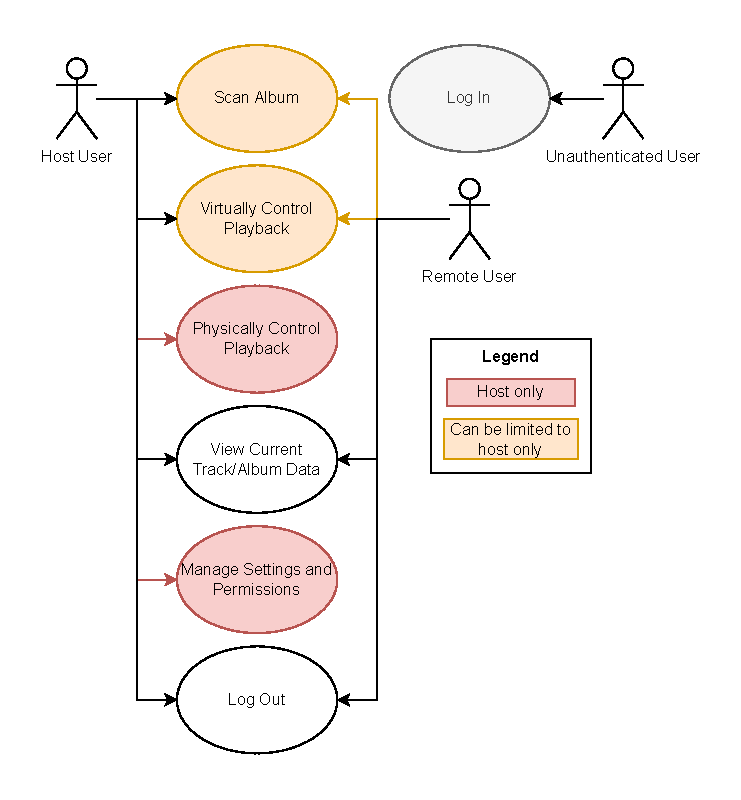
\includegraphics[width=0.65\linewidth]{images/UML_UseCase.pdf}
                \caption{A UML diagram of user use cases}
                \label{fig:umlusecase}
            \end{figure}
    
            \paragraph{Functional Requirements}
                \begin{itemize}
                    \item \textbf{FR1}: The system must identify album covers using image recognition with at least 90\% accuracy. This threshold balances feasibility and usability, ensuring reliable recognition without demanding unattainably high accuracy, based on similar machine-learning image recognition benchmarks (typical target: ≥85–90\%).
                    \item \textbf{FR2}: Album identification and music playback must start within 5 seconds. Five seconds represents a practical limit beyond which users begin to perceive the system as sluggish or non-responsive. This aligns with usability guidelines for interactive digital systems.
                    \item \textbf{FR3}: The system must retrieve corresponding music tracks from Spotify after successful identification.
                    \item \textbf{FR4}: Users must be able to control playback (play, pause, skip) via software interface.
                    \item \textbf{FR5}: The user interface must clearly display information about the album and track being played.
                    \item \textbf{FR6}: The interface must be intuitive and suitable for non-technical users.
                    \item \textbf{FR7}: The system must provide physical controls (buttons/dials) for basic playback operations.
                \end{itemize}
            
            \paragraph{Non-Functional Requirements}
                \begin{itemize}
                    \item \textbf{NFR1}: Total system latency (from recognition to playback) should not exceed 5 seconds.
                    \item \textbf{NFR2}: System reliability must ensure an operational uptime of at least 99\%. Ensures robust availability without requiring prohibitively expensive redundancy, aligning with standard reliability targets for consumer-oriented interactive systems
                    \item \textbf{NFR3}: Recognition failures should gracefully prompt user intervention without causing system crashes.
                    \item \textbf{NFR4}: The system must be fully compatible with Raspberry Pi 5 hardware.
                    \item \textbf{NFR5}: Setup and operation should be documented clearly, enabling ease of use without extensive technical expertise.
                    \item \textbf{NFR6}: The solution must adhere strictly to UK copyright laws.
                    \item \textbf{NFR7}: The system must comply fully with all used APIs' Terms of Service.
                \end{itemize}
            
            \paragraph{Constraints}
                \begin{itemize}
                    \item Implementation must accommodate the hardware limitations of Raspberry Pi 5.
                    \item Use of API data must adhere strictly to their licensing and usage terms.
                    \item The dataset used for training image recognition must comply with UK legal guidelines for non-commercial research.
                \end{itemize}
            
            \paragraph{Assumptions}
                \begin{itemize}
                    \item Users have consistent and stable internet access.
                    \item Users possess active required accounts for playback services, where needed.
                    \item Operational lighting conditions are sufficient for accurate image recognition.
                \end{itemize}
    
        \subsection{Pillars of Design Philosophy}
    
            The following core principles were adopted in, and guided, the design phase:
    
            \begin{itemize}
                \item \textbf{Platform Agnosticism} The system was designed to avoid reliance on any single external component, using hexagonal architecture (plugs and adapters) to allow interchangeable parts, mandating components all conform to common interfaces. Flexibility extended across both services and device types, aiming to support a broad range of OSes and hardware, emphasising the creation of a general solution.
            \end{itemize}
    
            \begin{itemize}
                \item \textbf{Physicality First} The device prioritises tactile interaction, echoing traditional vinyl players to maximise nostalgic appeal. Core playback controls must be usable fully with only the physical components; with digital enhancements remaining optional and unobtrusive.
            \end{itemize}
    
            \begin{itemize}
                \item \textbf{Digital Completeness} Every physical function is mirrored digitally to ensure full accessibility, particularly for users with impairments or lacking physical access. Though optional, the digital interface must integrate seamlessly; not to be treated as an after-thought.
            \end{itemize}
    
            \begin{itemize}
                \item \textbf{Open Source} With a firm belief in the importance and value of the open source community, the project will contribute, with all code being made public (subject to academic clearance), and all relevant aspects being clearly documented to maximise the usefulness of this project to others. Such tools and services were favoured where possible.
            \end{itemize}
    
            \begin{itemize}
                \item \textbf{Robustness and Maintainability} Emphasis was placed on clean, modular code using design patterns, single-responsibility principles, and comprehensive unit testing to ensure long-term reliability.
            \end{itemize}
    
            \begin{itemize}
                \item \textbf{Ethical Responsibility} The project was developed with ethical considerations at the forefront, accounting for copyright, transparency, responsible data use, and system security.
            \end{itemize}
        
        \subsection{System Architecture} % high-level system overview
    
            \begin{temp}               
                \begin{temp}Note from Sean: Discogs/Spotify should be together\end{temp}
                
                Data Flow Diagram;
            \end{temp}
    
            The final architecture design was to build a web application running on a single physical device, with both server and client hosted locally. Both physical analogue controls and exposed REST endpoints interface with the server, while the client handles audio playback and visual output. Communication between server and client occurs via both standard HTTP and bi-directional WebSocket channels, enabling real-time updates in both directions.
    
            The design incorporated a motor to spin a disc during playback, visually enhanced by matching visuals from the UI being vertically projected down onto the system, giving the appearance of a stylised vinyl with holographic overlays (e.g., current track information).
    
            Later in development, the architecture was extended to support remote clients. These external devices also connect via WebSockets, providing communal and accessible control, with the server updated to manage multiple concurrent connections (see Figure~\ref{fig:networkDiagram}).
        
            \subsubsection{Design Choices}
                % unique 1-1/1-many relation
                % server hardware control
                % host v. remote client
                \begin{temp}
                    Here should be the \textbf{justificatory} elements for the choices made: particularly the more broad, or weird, or niche choices. Very specific logical choices should be in their specific components.
                
                    For example:
                    \begin{description}
                        \item[1.] Why use a web approach for a localised device?
                        \item[2.] Why use an unorthodox 1-1 Websocket approach for client-server calls?
                    \end{description}
                    Also things such as 'point of truth handling', etc.
    
                    Is it a good idea to write this explicitly like an FAQ section, with the question stated, and then answer given?
                \end{temp}
    
                \paragraph{Why use a web approach for a localised device?} Despite being local, a webstack was chosen to align with streaming APIs and ensure device agnosticism. This also allowed easy expansions due to its network architecture, simplifying later expansion to remote access. Web tech also streamlined deployment without per-device setup and configuration being needed.
    
                \begin{figure}[h]
                    \centering
                    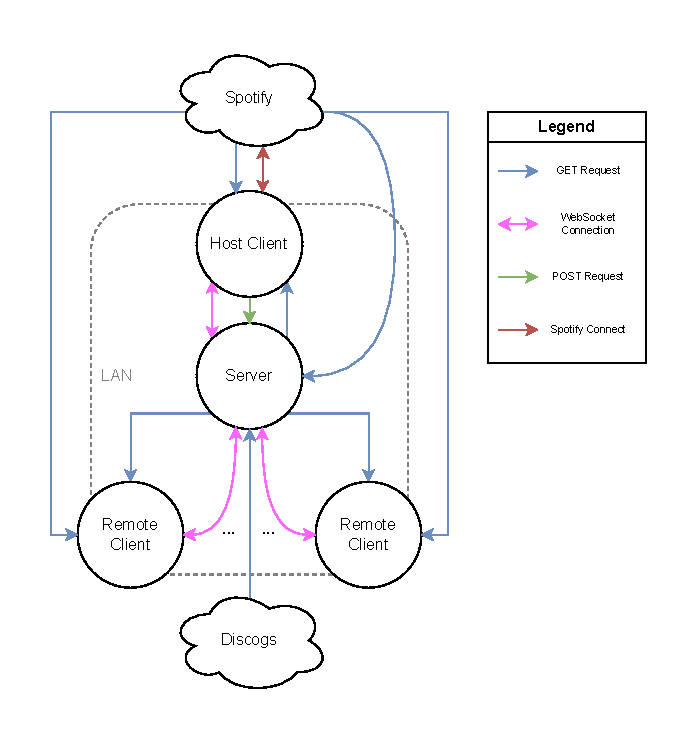
\includegraphics[width=\textwidth]{images/VTT_network.NetworkDiagram.pdf}
                    \caption{Network diagram of system. }
                    \label{fig:networkDiagram}
                \end{figure}
        
            \subsubsection{Technology Stack}
    
                \begin{temp}
                    Is this actually needed? All of these things are covered below. But, it seems good to have a concise high-level summary?
                \end{temp}
                
                \begin{itemize}
                    \item \textbf{Music Vendor:} Spotify Web Playback SDK --- selected for compatibility and prior familiarity, with an existing Premium account as required for integration.
    
                    \item \textbf{Frontend:} React, TypeScript --- chosen for type safety, efficient UI reactivity and strong SDK support.
                    
                    \item \textbf{Backend:} Python, FastAPI --- lightweight and ML-friendly, ideal for embedded deployment, in addition to be easyto use.
                    
                    \item \textbf{Build Tool:} Bun \& Vite ---  chosen for speed, easy rapid testing, and network hosting support.
    
                    \item \textbf{Hardware:} Raspberry Pi 5 --- selected for easy GUI interfacing with expansive modularity; latest available model used for optimal performance.
                \end{itemize}
    
    
        \subsection{Hardware}
    
            The system runs on a Raspberry Pi 5, chosen for its flexibility, general OS support, with sufficient processing power for using neural network models. Microcontrollers such as Arduino boards were too limited. Since the software was designed to be usable on any reasonable device, it required a general-use OS and web browser. The NVIDIA® Jetson Nano™ Developer Kit was considered, as it is a powerful AI-oriented chipboard, featuring an NVIDIA Maxwell architecture with 128 NVIDIA CUDA® cores. For running a neural network solution, this architecture is significantly more powerful than the Raspberry Pi 5's equivalent VideoCore VII GPU, which is primarily for graphics and not general-purpose GPU compute like CUDA. The Jetson Nano offered superior GPU acceleration, but its benefits were unnecessary for the relatively lightweight CNNs required by this system. Additionally, the Jetson had a higher cost, lower availability, and narrower general-use application range. The Pi 5 was deemed sufficient for the use case, and its broader community support made it the more pragmatic choice.
            
            Beyond functionality, aesthetics were key. In order to best utilise nostalgia, the device was designed to make use of a stylish mahogany wood with brass controls. Research shows that, in one survey, wood is the most frequently cited material in nostalgic household items, appearing in 34\% of nostalgic objects (with metal second at 21\%) \cite{Skinner2022}. These materials were ubiquitous in classic mid-20th-century audio equipment, so they instantly call to mind ``the charm of a bygone era'' \cite{LookInTheAttic2024}.
    
            \subsubsection{Hardware Components}
    
                It was essential to ensure all chosen hardware could be supported by the Raspberry Pi 5's GPIO pinout (see Figure~\ref{fig:RPi5Pinout}).
    
                \begin{figure}[htbp]
                    \centering
                    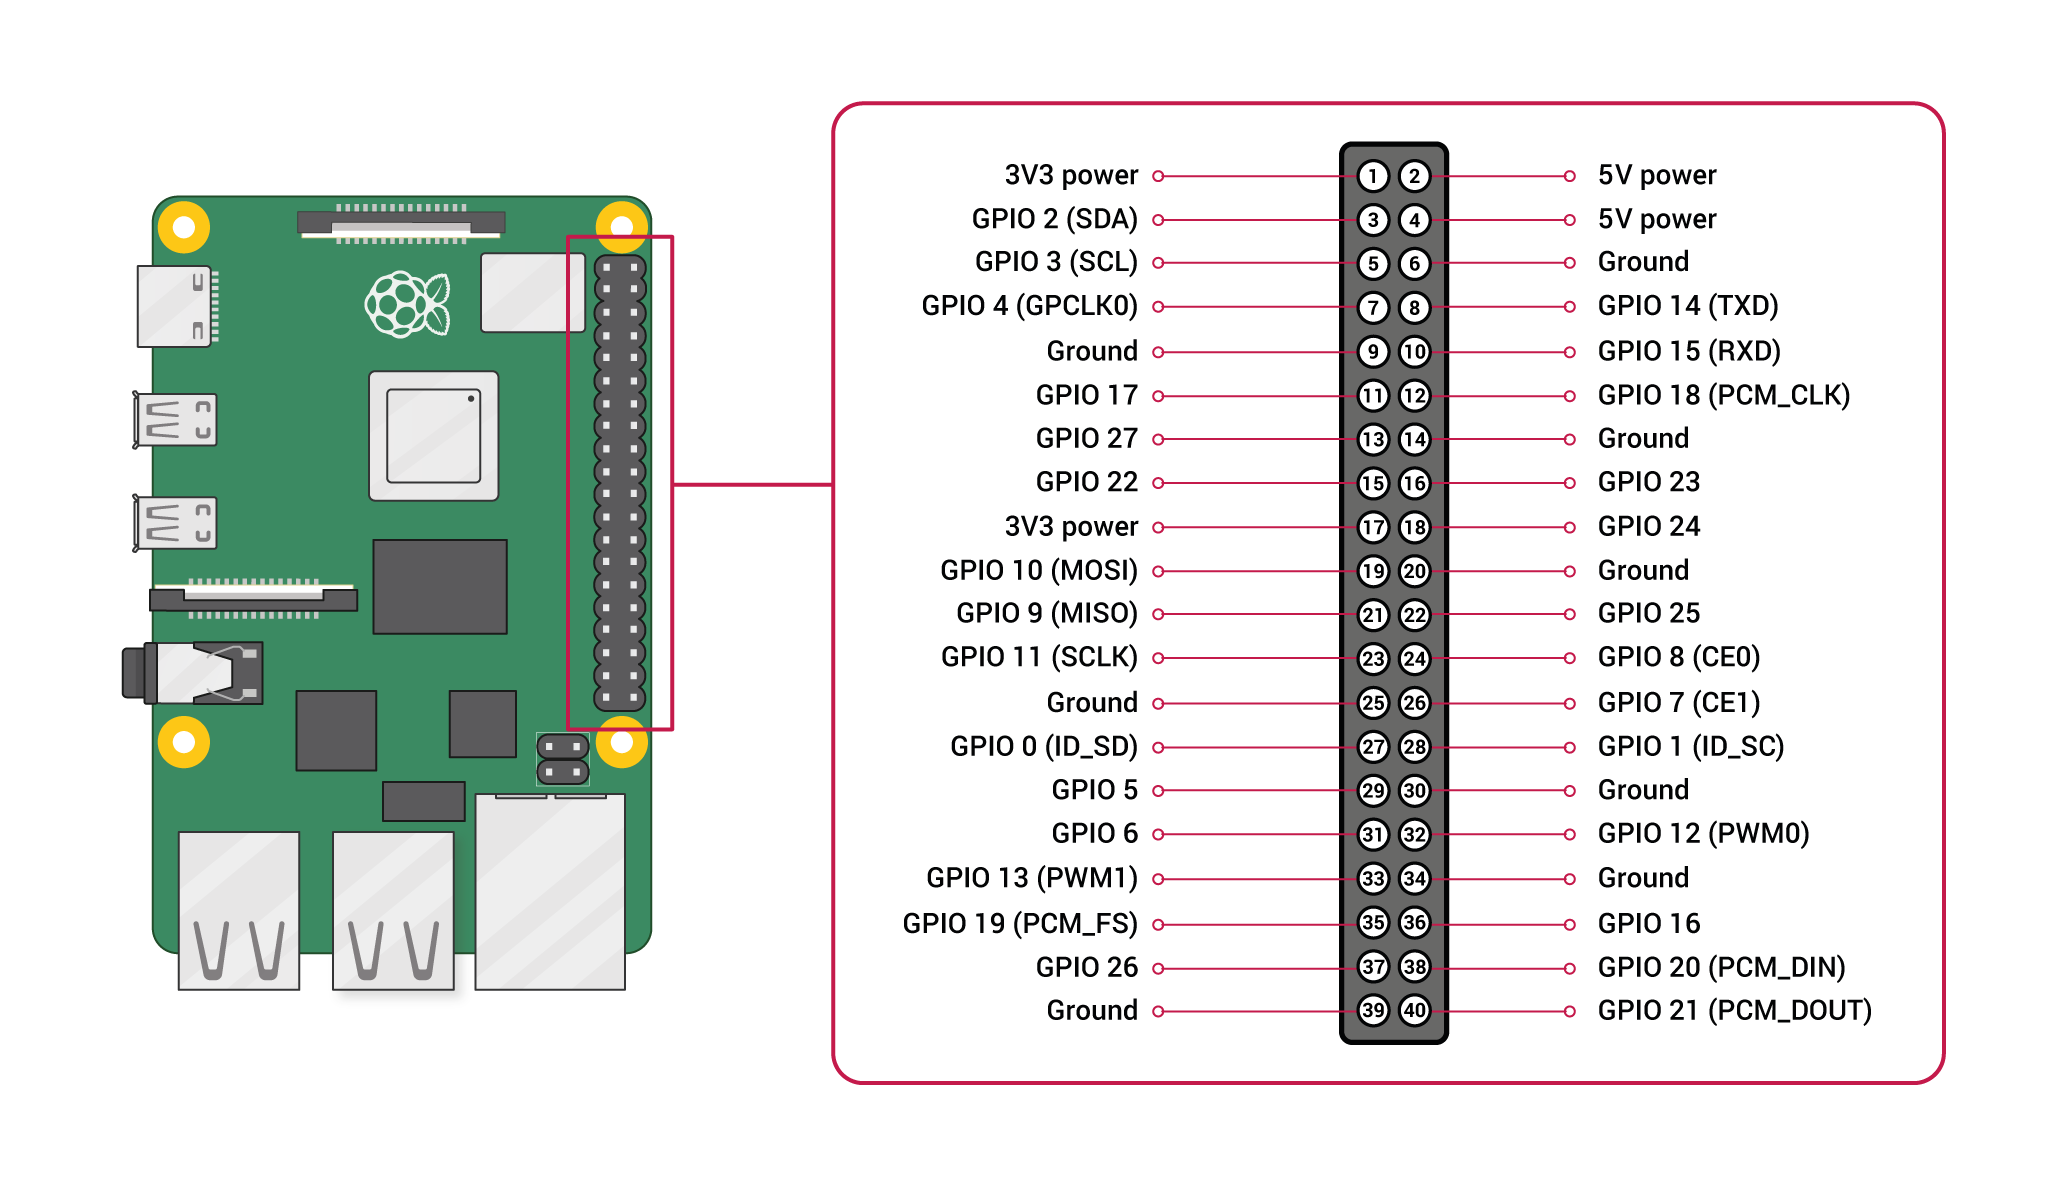
\includegraphics[width=\linewidth]{images/raspberry-pi-5-pinout.png}
                    \caption{Pinout configuration of Raspberry Pi 5}
                    \label{fig:RPi5Pinout}
                    \caption*{Source: \href{https://www.raspberrypi.com/documentation/computers/raspberry-pi.html#gpio}{Raspberry Pi Documentation}}
                \end{figure}
    
                Core components include a DC motor (via driver), rotary encoder switch, camera, and a trigger button (Table~\ref{tab:coreGPIOPins}). The rotary encoder supports vector input (direction + magnitude) and button presses, enabling a compact control scheme:
    
                \begin{itemize}
                    \item \textbf{Knob rotation}: adjust volume
                    \item \textbf{Button pressed, no rotation}: toggle pause/play.
                    \item \textbf{Knob rotation (button pressed)}: change to previous/next track, depending on direction.
                \end{itemize}
    
                \begin{table}[htbp]
                    \centering
                    \caption{GPIO Pin Requirements for Core Functionality}
                    \label{tab:coreGPIOPins}
                    \begin{tabular}{|l|l|l|}
                        \hline
                        \textbf{Component} & \textbf{Required Pins} & \textbf{Note}\\ \hline
                        \multirow{5}{*}{DC Motor (via Driver)} & 1 × 5\,V & Motor driver power \\ \cline{2-3}
                                                               & 1 × GND & Ground \\ \cline{2-3}
                                                               & 1 × 5\,V & Motor power \\ \cline{2-3}
                                                               & 2 × GPIO & Direction control \\ \cline{2-3}
                                                               & 1 × GPIO (PWM) & Speed control \\ \hline
                        \multirow{5}{*}{Rotary Encoder Switch} & 1 × 3.3\,V & \\ \cline{2-3}
                                                               & 2 × GPIO& Rotation data (CLK, DT)\\ \cline{2-3}
                                                               & 1 × GPIO & Button input (SW)\\ \cline{2-3}
                                                               & 1 × GND & \\ \hline
                        \multirow{2}{*}{Button (Camera Trigger)} & 1 × GPIO & \\ \cline{2-3}
                                                                 & 1 × GND & \\ \hline
                        Camera & 1 × USB or Ribbon Port & \\ \hline
                    \end{tabular}
                \end{table}
    
                Additional optional features included a hinged arm switch for playback control, offering a large, tactile alternative better suited for accessibility and immersion; a motor-mounted encoder for stall detection, preventing burn-out; and a second camera for scanning back covers (Table~\ref{tab:optionalGPIOPins}). These additions enhance safety, robustness, longevity, and engagement. While the dynamic knob offers fine control, its complexity may be a barrier -- mitigated by the simpler hinge mechanism, expanding user interaction options.
    
                \begin{table}[htbp]
                    \centering
                    \caption{GPIO Pin Requirements for Optional Components}
                    \label{tab:optionalGPIOPins}
                    \begin{tabular}{|l|l|l|}
                        \hline
                        \textbf{Component} & \textbf{Required Pins} & \textbf{Note}\\ \hline
                        \multirow{5}{*}{Rotary Encoder (Motor Stall Detection)} & 1 × 3.3\,V & Sensor power (VCC)\\ \cline{2-3}
                                                                                & 2 × GPIO & Rotation data (A, B) \\ \cline{2-3}
                                                                                & 1 × GND & \\ \hline
                        \multirow{2}{*}{Hinge Switch} & 1 × GPIO & \\ \cline{2-3}
                                                      & 1 × GND & \\ \hline
                        Secondary Camera & 1 × USB or Ribbon Port & \\ \hline
                    \end{tabular}
                \end{table}
    
                All components fit within the Pi 5's GPIO limits (Table~\ref{tab:pinSummary}), with a reasonable number of redundant pins to accommodate potential failures and room for expansions. However, all 5\,V pins are used; though, if needed, motor power can be offloaded to an external supply, which would free up one of these pins.
    
                \begin{table}[htbp]
                    \centering
                    \caption{Summary of GPIO and Port Requirements vs. Availability}
                    \label{tab:pinSummary}
                    \begin{tabular}{|l|c|c|c|c|}
                        \hline
                        \textbf{Pin / Port Type} & \textbf{Core}& \textbf{Optional}& \textbf{Total Required} & \textbf{Available} \textsuperscript{see Figure~\ref{fig:RPi5Pinout}
    }}\\ \hline
                        5\,V Power & 2 & & 2 & 2 \\ \hline
                        3.3\,V Power & 1 & & 1& 2 \\ \hline
                        GND & 3 & 2 & 5 & 8 \\ \hline
                        GPIO (Standard) & 6 & 3 & 9 & 28 \\ \hline
                        GPIO (PWM-capable) & 1 & & 1 & 4 \\ \hline
                        USB or Ribbon Port & 1 & 1 & 2 & 2+\textsuperscript{*}\\ \hline
                    \end{tabular}
                    \caption*{\textsuperscript{*}Raspberry Pi 5 supports 4× USB + 2× camera ribbon ports.}
                \end{table}
    
            \subsubsection{Operating System}
    
                Raspberry Pi OS (or just RPiOS; formerly Raspbian), is an operating system produced by the the Raspberry Pi Foundation as the official OS for their chipboards. This makes interfacing with components such as GPIO pins seamless and easy. However, in order to make the system as hardware-agnostic as possible, a standard Ubuntu kernel was used for the project. This forced solutions to not rely on native Raspberry Pi interfaces, and so, whilst it made certain aspects more challenging, it means than the project is not locked to the RPi hardware.
    
                Ubuntu is also fully open-source, unlike RPiOS, which has some proprietary aspects.
    
                Firefox (also open-source) was used during development (as Ubuntu's default browser), with Chromium tested periodically to ensure cross-browser compatibility.
                
        
        \subsection{Front-end}
            \subsubsection{Primary User Interface}
                % lofi designs
    
                \begin{temp}
                    - Physical user interaction controls
                \end{temp}
    
                \begin{temp}
                    UI Wireframes / Mockups
                \end{temp}
    
                React was chosen for its strong support of reactive state updates from multiple sources -- crucial for the host client, which must synchronise state changes from its internal user interface, external streaming vendor, and the server (see Figure~\ref{fig:statePropagationDiagram}). Prior experience with the framework was also an influence.
            
            \subsubsection{Audio Playback}
                % Spotify Playback SDK
                % Spotify Web API
    
                To maintain platform agnosticism, all streaming and metadata APIs are accessed through abstract interfaces, allowing seamless interchangeability through their uniformity. Spotify was selected due to prior experience, existing subscription, and ease of integration, with both front- and back-end components using its Web SDK.
    
                For implementation, only one external streaming API was selected to be implemented. After considering various options, Spotify was chosen due to past experiences with the system making it faster to integrate. In addition, most services required a subscription with the service in order to stream them; a pre-requisite already met for Spotify. For these reasons, Spotify was chosen for the audio streaming in the front end component, and thus, the corresponding back-end systems also used Spotify.
    
            \subsubsection{Minimal UI}
    
            Following the decision to build a single physical device, the UI was designed to be minimal and non-interactive by default -- entirely operable without a mouse, input, and screen. In order to emphasise the physical-first design, in a unobtrusive way, GUI buttons and sliders remain hidden unless the mouse was recently in motion, offering an easy fallback control. The UI mirrors the capabilities of physical controls and also further allows configuration of settings, including remote access permissions and motor toggling (available for the host only, see \ref{sec:security}).
    
            It was important to ensure that the UI offered no less control and/or information as the physical controls did.
    
            Customisation of the UI was also an important aspect. As the physical device could vary between owners, user's should be able to set the proportions of the projection area, for example setting the baseplate's ratio, and the position and size of the disc. This would not only better accommodate different devices and setups (if the projector is closer, everything should be scalable to be smaller), but also allows creative expression for the user in letting them decide how to set up their system -- emphasised by even being able to disable the motor, if the user wants a quieter option.
        
            \subsubsection{Remote Clients}
    
                \begin{temp}
                    - for convineince, the need for (33-45) adapter  can be cited
                    % https://external-content.duckduckgo.com/iu/?u=https%3A%2F%2Fnotesonvinyl.com%2Fwp-content%2Fuploads%2F2022%2F04%2Fspeeds-of-the-different-record-types-1.png&f=1&nofb=1&ipt=7d1e31af8468ae7ae70f11be6bd40c897a73cf0c42aa194a5e09309f9af25945&ipo=images
                    % https://external-content.duckduckgo.com/iu/?u=https%3A%2F%2Fwww.bluescentric.com%2Fimages%2Fproduct%2Flarge%2F557_2_.jpg&f=1&nofb=1&ipt=1cd939744050d9f13eb7f581b786a2f22d3787cf30dd60c2a6975a816043546f&ipo=images
                \end{temp}
    
                During development, the system was extended to support not only local browser access on the host device but also remote access from external devices such as mobile phones and computers. This decision was motivated by both accessibility and convenience. For users with physical impairments, remote access via phone allows full operation without needing to interact with hardware controls. It also enables users without required peripherals -- such as the camera -- to use their phone’s camera for album scanning, instead of preventing this functionality.
    
                Remote access further supports communal interaction: multiple users can simultaneously connect, control playback, or queue music, creating a shared experience. It also preserves some degree portability from the original mobile concept -- users can scan an album when away, and upload it to the system when they are next connected, instead of relying solely on real-time images from cameras.
                
                Rather than implement a separate front-end or routing system, the client was implemented as a single-page application, with the UI adapting based on whether the device is the host or remote, determined via a server query. This also maximised component re-usability, to help ensure the system was robust without major additional testing being required.
                
                The remote interface mirrors the physical controls' functionalities, offering playback (play, pause, skip, previous), volume adjustment, album scanning, and even access to the host's owned album library, which can be browsed or shuffled. Remote users can perform any action available to those physically interacting with the device.
    
        
        \subsection{Back-end}
    
            A centralised server was required to coordinate communication between multiple clients, handle physical controls, run album detection (see Section~\ref{sec:mlDesign}), manage authentication (see Section~\ref{sec:security}), and orchestrate system logic.
    
            Python was chosen for its simplicity and strong ML ecosystem. FastAPI, with Uvicorn, was selected as a lightweight, async-friendly framework suitable for the Pi.
    
            The server uses the singleton pattern to ensure the machine learning model loads only once. While scalability wasn't a primary concern, following this and the Single Responsibility Principle ensured a modular, maintainable codebase -- e.g., separating API routes, authentication logic, and control systems into distinct classes.
    
            As the server also handles the physical controls (in addition to needing to relay commands from the remote clients, as per Figure~\ref{fig:statePropagationDiagram}), the server needed to be able to instantaneously communicate with the clients. Rather than relying on inefficient polling, or the one-way, text-only approach of using Server-Sent Events (SSEs): websockets provide great flexibility in allowing the client and host to both communicate with each other, bi-directionally, with minimal delay and resource usage. This is ideal, because whilst the server will sometimes need to update the client (when a user uses a physical control, for example) there will also be times where the client systems need to update the server (for example, if the music is paused directly through Spotify, from a device not connected to our server, the server needs to be informed of this by the host client). Using this bi-directional channel ensures that all similar communications go through the same context, and avoids needing to implement similar code multiple times, in different ways (such as if this was done with standard REST calls and SSEs).
        
            \subsubsection{Metadata Retrieval}
                % Discogs API
                % assert Discogs ToS compliance (not used for AI)
    
                Traditionally, when a track or album is playing, online streaming services show the cover art to the user. Since this project relies on scanning a cover art in order to play the music, it seemed redundant to broadcast the current track by showing the user the same artwork they have in their hands. So, rather than duplicating this, and in order to lean more into the physical vinyl concept, the server was designed to fetch the centre label of the corresponding vinyl, in order to show this on the disc, instead.
    
                In order to fetch this, Discogs' API was used, as they maintain a carefully curated library of many images for vinyls, including high-quality images of these labels. Whilst Discogs do not allow their images to be used in AI systems, they can be used if strictly processed by traditional CV methods. Using Hough Circle detection, the image library of the relevant album can be scanned for the best-fitting circle, which, then cropped, can be served to the front-end.
          
        \subsection{Machine Learning Model Design} \label{sec:mlDesign}
    
            Based on the background research, a machine-learning approach was chosen over tailored OCR or feature extraction methods, as album covers can often lack text and vary widely in design. While visual transformers have the best performance best on large datasets, a smaller CNN was selected to better converge on the more limited and specific dataset of albums used here.
        
            \subsubsection{Dataset Collection}
                % use of CoverArtArchive
    
                A suitable dataset was required for training. Manual image collection would be slow and risk bias, and most services (e.g., Spotify, Discogs) prohibit using their assets in AI systems. Last.fm’s terms posed no explicit restrictions, but the Cover Art Archive (via the Internet Archive and Musicbrainz) was selected due to its open licensing in addition to the inclusion of images of the backs of covers -- something other platforms lacked.
    
                To ensure unbiased validation, manually photographed images were still collected separately, though to a limited extent due to physical availability constraints (see~\ref{data:val}).
    
            \subsubsection{Solution Design}
    
                The core aim was to classify scanned album covers using a CNN. To detect cases where no album is present (e.g., the camera triggers too early), a ‘null’ class of random images was included. These would be carefully curated to avoid distorting the classifier’s behaviour. However, since the system runs on a single, static device, the camera’s background is expected to remain stable -- allowing this null class to instead reflect the actual backdrop seen when no album is present.
    
                This stability could be further leveraged using temporal background subtraction: averaging multiple frames over time to generate a 'baseline' image. Subtracting this from new frames would help detect the presence or absence of an album, and also prevent the background influencing predictions (e.g., small albums revealing too much background).
    
                If null classification works well, the camera could continuously poll images and automatically react when a new album is detected — removing the need for manual input. However, this would be an optional accessibility feature, as the physical act of taking a photo was seen as an important, engaging element.
    
                To further increase robustness, the system could not rely solely on the CNN. If classification confidence is low, fallback to OCR and barcode scanning could better inform the decision, or even address it entirely. This combinatorial approach helps account for edge cases and albums outside the model's training data. Confidence thresholds would need to be tuned through experimentation.
    
                \begin{temp}
                    Decision Flowchart for Image Recognition
                \end{temp}
        
            \subsubsection{Model Architecture}
    
                A CNN was used for its proven ability in image classification. The design followed an educational, iterative approach: starting with a minimal model, then incrementally expanding and tuning it based on performance.
                
                The goal was to create a few different models, with differences in architecture to experiment to find results. Other than broad decisions, their architectures were not developed until during implementation. The details of each of these models is described in Section~\ref{sec:mlImp}.
    
                However, three conceptual models were created. In order to distinguish between these models beyond just their most basic architecture, each was given a unique name. The inspiration for these names were taken from Greek mythology, using the names of snake-likes creatures (see Appendix~\ref{app:Greek}, for more details).
    
                \paragraph{Ouroboros} A standard feed-forward CNN, designed for closed-world classification of known album artwork.
    
                At this most basic level, the goal is to simply design a model that can accurately learn information from both a small and large dataset of albums, to ensure that it can handle varying collection sizes of different users.
    
                Since the task of learning albums from their artworks is a closed-world scenario -- that is, the model is expected to classify inputs that are nearly identical to the training examples, with minimal variation, since two versions of the same album usually have identical artworks -- the need for generalisation is low and the model can rely more on memorisation. This `memorisation-friendly' nature of the task was the inspiration for the name Ouroboros, the self-eating serpent.
    
                \paragraph{Amphisbaena} A dual-headed neural network, trained to capture and classify an image's most likely artist, in addition to the album itself.
    
                If the Ouroboros model is viable, then it was desired to experiment with adding multiple heads, so that the model could predict an artist, even if it had not been trained on a specific album. If an artist can be predicted with high confidence, but no album is overly confident, then this could be used to aid the fallback logic, alongside the OCR/barcode data, etc.
    
                Additionally, through further experimentation, this could be expanded to learn genre, or even the decade of release.
    
                \paragraph{Hydra} An expandable architecture supporting the addition of new classes without retraining the entire model.
                
                % An adaptive multi-headed model, allowing the creation of new heads through knowledge distillation and consensus to learn new, previously out-of-scope classes, whilst still maintaining precision on previously trained data.
    
                A significant issue with using a closed classification system, is that any classes not included inside the training dataset can never be predicted. Whilst it is common practice to re-train (or fine-tune) a model, to adjust weightings based off of new data, the task of adding a whole new class to the model's options when deciding is a much more complex task.
    
                The most simple option is to simply re-train the whole model, with the original and additional classes and data. However, in order to best maintain fair dealings, all images used in training were deleted after use, by the system. Therefore, unless the user was to re-download the entire dataset each time, this was not a very viable option. Additionally, it could be the case that the online source of images may have had images removed, and therefore, re-training could actually offer worse performance in some cases.
    
                An aspiration target of model development for this project was to create a progressive neural network (PNN) that could adapt to new classes. The simple goal would be for the model to support a dynamic number of heads, and when new classes are added to train a new head using knowledge-distillation from previous heads (to prevent 'forgetting' previously trained classes), whilst still associating with the new classes. Once the new head is trained, it can be appended to the model, and a weighted consensus of the various heads would be used to determine the class.
    
        \subsection{Security Considerations} \label{sec:security}
            % handling of auth tokens (transient)
            % off-handing of persistence tasks
            % network hosting
            % option of same-user or any-user controls
            % API compliances
    
            \begin{temp}
                Security Architecture Diagram
            \end{temp}
    
            \begin{temp}
                Data Flow Diagram
            \end{temp}
    
            Whilst this system is designed as a local device, with the only connectivity to external sources being trusted APIs, security was still an important consideration, and taken seriously within each phase of the project.
    
            \paragraph{Handling of secure data} Since this project integrates with external systems, proper authentication token handling was required. Especially when serving multiple users simultaneously. The system follows a standard RESTful token flow, wherein a client is redirected to the server through the external service's callback, with a token that can be used to request a formal authentication token. This token is stored only in the server's memory, and is associated with the client's session ID cookie. Therefore, a user can only fetch an authentication token through the GET endpoint if they are the same device that made the request. This ensures secure data was only accessible to authorised parties.
    
            \paragraph{Persistence task off-handing} Some tasks require non-volatile storage, for example: storing a list of the albums a user has scanned into their 'collection'. The decision was made that, where possible, non-sensitive data should be off-loaded onto the API service being used. That is, rather than store the list of songs locally, a Spotify playlist can be created and updated as the system's 'file'. This meant all GDPR compliance needed to be met by the external vendors, rather than this system.
    
            \paragraph{Local network hosting} To handle remote clients, it was decided to allow the front-end runner (Vite) to use a feature called network-hosting. This feature allows LAN devices to connect to the site. Whilst opening access to certain ports to same-network devices can have consequences, as a static device, this system is designed to only be used in a secure network (such as the user's house), and so no major actions were taken, beyond ensuring firewall services did cover the relevant ports.
    
            \paragraph{Command permissions} It was decided that even if user A was signed in on the host device, user B should be allowed to pause, play, scan, etc. from their external device if, and only if, user A authorises this. To achieve this, not only are the required UI buttons disabled when the host has disabled remote access, but all server-side logic enforces this. The host can either disable all remote connection, or allow only the host's account to do this, or allow all devices to access the server. The validation for is a user is the host or not, is done through the session ID cookies and verifying with the external API that the associated token is for the authorised user. Therefore, this cannot be ignored by a malicious user.
    
            \paragraph{API compliances} An intentional effort was made to ensure that all data processing, requests, and request-frequencies were compliant with the respective APIs' terms of services, rules, and limitations.
        
        \subsection{Testing Methodology}
    
            \begin{temp}
                Design of tests and evaluations; plan for unit testing, model evaluation, etc.
                
                Does the system satisfy that physical and aesthetic desires of that the vinyl trend appeals to, whilst still offering functional convenience over original systems?
            \end{temp}
            
            \subsubsection{Validation of Effectiveness}
    
                In order to evaluate if the developed solution is effective in reaching its goals, three primary metrics will be used:
    
                \paragraph{Model Performance} In order to assess if the model performs adequately, formal model evaluation will be performed. Two units will be under test: the recognition model and the metadata retrieval (the centre label, etc.). In order to assess the model's performance, a fresh test set of data will be used, of front-only photos of physical covers, from which an F1 metric can be calculated. Aditionally, the centre label accuracy can be objectively assessed by running it over a known set of albums, and manually comparing the accuracy compared to that of the owned vinyls.
    
                \paragraph{Usability} An important goal is whether or not the system and it's physical and digital controls are accessible and useful for users. To assess this, a user-centric approach will be taken, with evaluation of survey results\footnote{The evaluation form is accessible at \href{https://forms.gle/DS8oik9Vyny6Zxnk6}{https://forms.gle/DS8oik9Vyny6Zxnk6}} of people who have used the finished system.
    
                \paragraph{Code Robustness} In order to ensure code is functional, and to try to maximise its robustness, a full unit test suite will be developed in parallel. This suite will aim to have high code coverage.
        
            \subsubsection{Validation of Affectiveness}
                
                In addition to the practical side, the emotional value of the system also needs assessment. In order to ensure that the system has correctly appealed to its intended audience and to evaluate how well the system captures the appeal of traditional vinyl systems along with the convenience of a digital player, the user survey will also include questions regarding these aspects.
    
    %%%%%%%%%%%%%%%%%% SECTION 4 %%%%%%%%%%%%%%%%%%
    \section{Implementation}
        % details realised in practice
        % challenges, and how overcame
        % code-level or system-specific decisions, optimizations, or trade-offs
        % integration
    
        During development, several changes and refinements were made in response to practical challenges and emerging opportunities. While the original design served as a strong blueprint, some technical and hardware constraints necessitated creative problem-solving and re-evaluation of certain assumptions.
    
        This section describes the practical implementation of the frontend, backend, hardware, and machine learning components. It highlights key deviations from the design, integration details, and specific trade-offs made during the build process.
    
        \subsection{Front-end}
    
    
            The implementation of the front-end system was relatively smooth, largely due to the minimal-UI aspect of the design. The interface was designed to be practical first, with little-to-no creativity or flair being added until late in development.
    
            Was the product was functional, some polish aspects were added. For example, when an image is taken/uploaded to the system, it is briefly displayed on the screen before being 'lifted up' to unveil the vinyl and its centre label underneath.
    
            \subsubsection{Frontend Personalisation and Audio Effects}
    
            An alternate local audio player was developed alongside Spotify integration, enabling playback of user-stored files. This addressed notable gaps in Spotify’s catalogue—particularly rare or compilation vinyls—and also allowed the system to function in an offline setting, independent of internet connectivity.
    
            To enhance the user experience and evoke the character of physical media, a feature was introduced to overlay randomised noise and static onto locally played tracks. This added a perceived ‘warmth’ commonly associated with vinyl playback, offering a more personalised and nostalgic feel across different devices.
            
            Due to Spotify’s Terms of Use, such modifications could not be applied to streamed content, as altering or layering audio over Spotify’s output is strictly prohibited. However, for locally stored files, no such restrictions applied.
            
            As a basic proof of concept, a static noise layer was generated and played throughout the track, with subtle fluctuations in volume. The noise profile was determined using a hashed seed based on track metadata and playback time, ensuring variation across devices and tracks, while maintaining consistency for repeated plays by the same user. This meant that even the same audio file would sound slightly different depending on the user and device. The concept could be extended to introduce additional artefacts -- such as scratches, pops, or pitch modulation -- to more closely emulate the idiosyncrasies of vinyl.
    
            Much later into the project's lifecycle, when testing and evaluating the product, it was realised that a nail could be mounted onto the `arm' switch to better visually mimic a record player's needle. This even further improved the likeness beyond just the visual, as the nail scraping along the disc's surface created a scraping noise -- unique to the user's nail and grooves on the vinyl being used a projector surface -- without violating Spotify's terms of not overlaying other sounds\footnote{Appendix~\ref{sec:nailArt} explores some tangential thoughts on the final result of using this solution.}.
        
            \subsubsection{Challenges Encountered}
    
                \paragraph{Responsiveness vs. Wholeness} During development one challenge that was encountered was the latency that would sometimes occur in fetching a track's metadata after the track had started playing. In order to give the user as seamless of an auditory experience as possible, it was best to let tracks play instantly, with no delay. However, this meant that sometimes the centre label would be blank briefly before 'popping in' afterwards. Generally, UI principles dictate that an aspect should be loaded in completeness before rendering, to avoid unstable changes being displayed to the user. Since the system is primarily an audio system, it was decided to favour responsiveness, allowing the system to asynchronously update the interface if and when it got the metadata. However, in order to mitigate the pop-in, once a centre label is found the image was cached in the file-store, to prevent this search process being conducted each time. Furthermore, the aforementioned image display covering the vinyl, gives more of a chance for the pop-in to be hidden from the user, for those few seconds.
    
                \paragraph{DRM Issues} One notable issue came from the choice of the system's hardware. Raspberry Pi SBCs use ARM-based processors. Whilst Ubuntu is designed for this, a notable absence is that Google's WideVine DRM (which is used by both Firefox and chromium-browsers alike) does not have an official AArch64 build, which is needed for a RPi. The absence of a DRM meant that Spotify's audio could not be streamed in the browser. Whilst no AArch64 build exists in the official repos, there is, however, an official build used for ChromeOS systems. It was possible to install and use this version, which enabled DRM content on the Pi. However, if this had not been available, then this would have been a serious hurdle for the project's chosen system architecture.
    
                Additionally, there were some issues with missing media codec's in Ubuntu's default packages. This was easy to resolve, however, added more steps to the setup process, which required a greater need for documentation. This would have been minimised if using more established solutions, such the official Raspbian image on the Pi, or a proprietary OS such as Windows on an x64 board.
    
            \subsubsection*{Reflection}
                The minimal-UI approach streamlined implementation and fit the aesthetic aims, but surfaced UX quirks like unclear hidden controls. DRM limitations on ARM were an unexpected hurdle — thankfully overcome — but highlight a fragility in relying on vendor ecosystems.
    
        \subsection{Back-end} % maybe Front/Back should just merge to software, here
    
            The backend was developed with Python's FastAPI and asyncio libraries to maximise the performance of parallel tasks. In addition to this, PyTorch (see \ref{sec:mlImp}) and OpenCV were used to make the machine learning and image extraction processes simpler to perform.
    
            \paragraph{State Management}
            One interesting feature of the system, was that a state-propagation system essentially had to be created. Since the system can be split into three components (host client, remote client, and server), which also integrate with external systems (such as Spotify), all of these components had their own internal state which informed the system how to act, but needed to be writeable from the other components. The solution to this was to essentially create a reactive system, inspired by React's state and hooks system. All active components are linked in a linear chain (see Figure~\ref{fig:statePropagationDiagram}), therefore, other components states can be seen as dependencies. Each component is only concerned with updating adjacent components, when its internal state changes, and so, whenever a state change occurs in a component, it broadcasts this to its connected neighbour(s). This creates a real-time feedback loop, allowing changes, even from an external device using the official Spotify app, for example, to be synchronised with the motor's state. For each aspect, a single 'point of truth' was determined, and in cases where new connection are established, this was used. For example, the audio is playing through the host client app, and so, if there is a conflict of states, the host client's state is favoured.
            
            \begin{figure}[h]
                \centering
                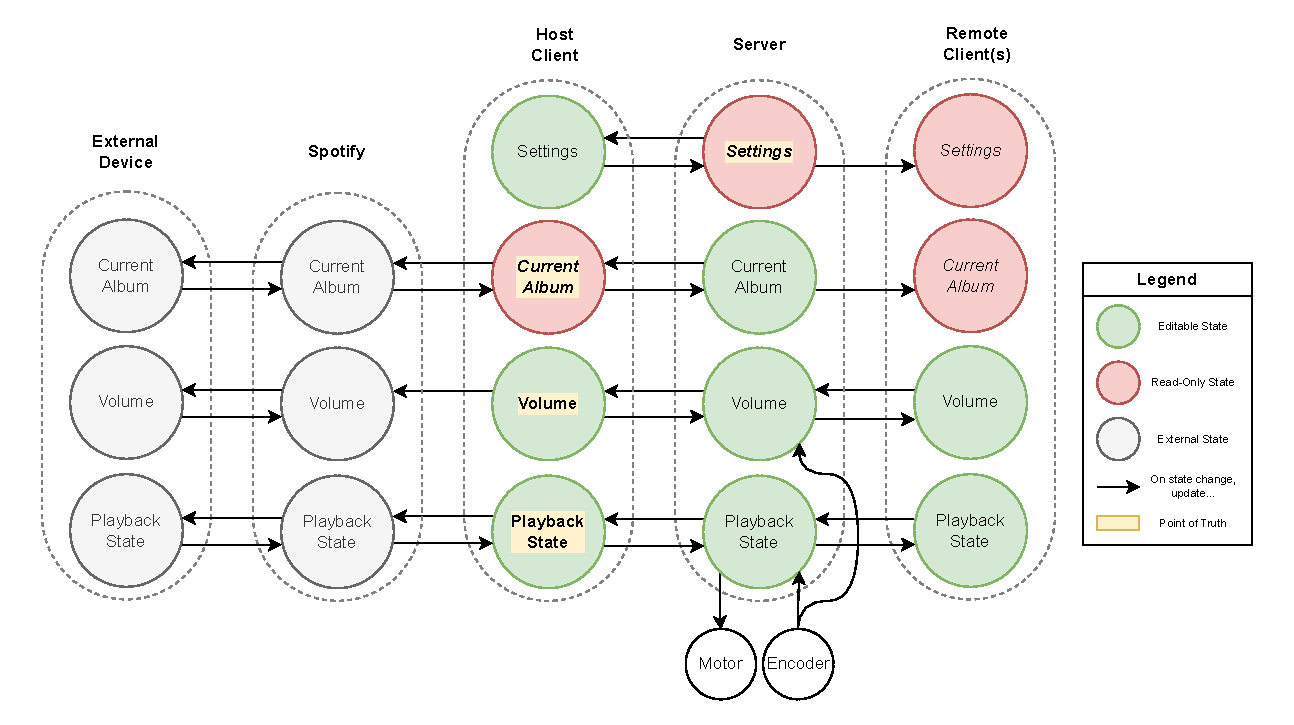
\includegraphics[width=\textwidth]{images/VTT_states.DependencyGraph.pdf}
                \caption{Dependency diagram showing state propagation model between both system and external components, allowing real-time reactivity to state changes from multiple sources.}
                \label{fig:statePropagationDiagram}
            \end{figure}
    
            One complication of this feature, was that there were often superfluous broadcasts. For example, if component A updated component B, then it is wasteful for component B to broadcast that same change back to component A. However, most of these broadcasts were kept, as it essentially created a 'handshake' system where components were not only updating each other, but received confirmation that those updates had been performed. The exception to this was in the front-end clients, where external and internal changes were flagged, to ensure that only internal changes were broadcasted. This was important because React's state system already handles state tracking, and could cause infinite feedback loops, throttling performance and the system's communication bandwidth. Additionally, since the host client interfaced directly with external components, it was best to avoid 'spamming' these components, which could result in timeouts.
    
            \paragraph{Alternate Processes}
    
            An important consideration was supporting multiple triggers for the same process—for instance, initiating album detection and playback via either a physical camera button or image upload from a remote device (see Figure~\ref{fig:imageSequenceDiagram}).
    
            \begin{figure}[h]
                \centering
                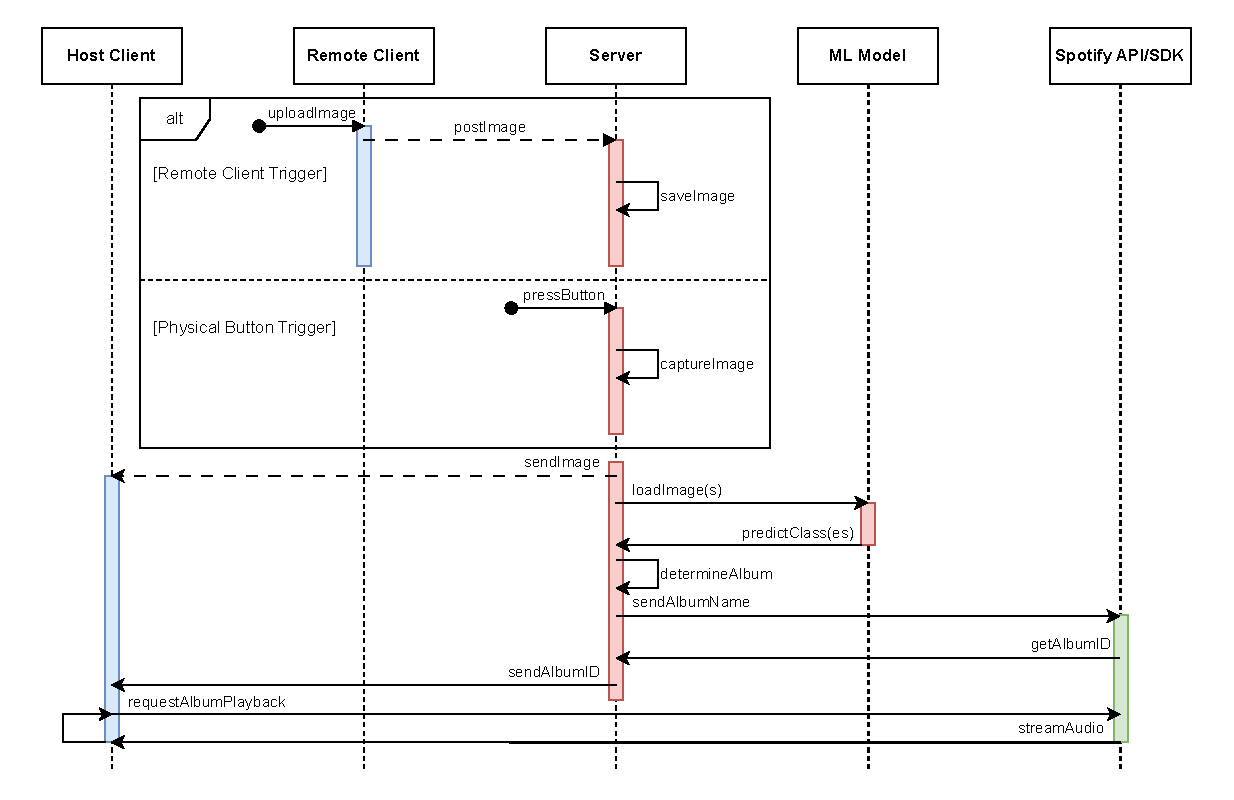
\includegraphics[width=\textwidth]{images/VTT_imageScan.SequenceDiagram.pdf}
                \caption{Sequence diagram showing two alternative triggers (client upload and server capture) leading to image processing and metadata retrieval before sending playback instructions to the host.}
                \label{fig:imageSequenceDiagram}
            \end{figure}
    
            In order to maximise the code's maintainability, re-using the code for the shared part of the process was of utmost importance, however since one trigger was an asynchronous REST endpoint, and the other a low-level polling of hardware. This would have been very difficult to manage if these functions were not in isolated components. Keeping with SRP practices, as decided early on, prior to any development, helped accommodate these mid-implementation changes to the system, with minimal complications.
    
            \paragraph{Metadata Retrieval}
    
            When fetching the centre labels from Discogs, using a simply query generated from the Spotify metadata, the images are downloaded and analysed one-by-one, aiming to find a one of a suitable 'roundness'. In order to get an image selected and server to the host client as fast as possible (maximising responsiveness in the system), the first suitable image is used, rather than searching all images for the best candidate. A very simple solution was implemented, using manually-defined parameters for a Hough Circles search, based off of the known proportions of centre labels. This made the system less robust than using a dynamic/generalised search, however, caution was taken to respects Discog's prohibition of their data for machine learning systems-- which is a vague term and arguably any automated computer task could be classified as. This system would benefit from better implementation, with two major improvements being searching the whole image library, and simply updating past results; and using a more dynamic search technique, looking for a dynamic number of circles, and perhaps using gradient detection to only find 'harsh' circles (colour on black), since vinyls tend to be black. Additionally, we could exclude circles that do not encompass a smaller circle, as all vinyls (and therefore, their centre labels) have a small hole in the centre.
    
            \subsubsection{Challenges Encountered}
    
                \paragraph{Authentication handling}
    
                Once the system was changed to allow multiple devices to connect, the whole authentication flow for the server had to be re-written, as it was initially built on the assumption that it would only ever be a single local connection being used. Whilst this required some work, it was a good reminder during the process to challenge the assumptions made during development, and no other changes as large as this had to be made later on in the process, due, at least partially, to this learning experience.
    
                \paragraph{Removal of Barcode Scanning}
    
                It was realised early on that, whilst covers do often have barcodes on their backs, which can uniquely identify the exact album: these barcodes are too low quality to ascertain information from in a image of a full album, without very high quality cameras, which this project did not want to utilise, to avoid reducing the technical accessibility of the system. It could have been setup so that, if a user's scan fails, they can optional re-scan, but this time closer to the image, so that it is just the barcode being captured, but even then, testing found that barcodes are very weak against noise and lighting conditions for general optical cameras (largely due to the fact that they only have one level of redundancy). Some vinyls have QR codes, which are much better suited for general scanning, however, there is no widely adopted system for how a record's QR code correlates to the album (oftentimes it is just a redirect to merch store, etc.). Furthermore, having to position the cover in a specific place, made the system more fiddly than convenient, and so this option was dropped entirely.
    
                \paragraph{Change of Spotify Security Requirements}
    
                In mid-February, near the end of development, Spotify announced it would remove support for HTTP callback URIs in favour of HTTPS from the 9th of April \cite{spotify2025security}. This posed a challenge, as the system had used HTTP under the assumption it would only run locally in a development-like environment. As compliance with API requirements was essential, this change had to be accommodated, despite the codebase being effectively frozen aside from bug fixes.
    
                Switching to HTTPS caused several regressions and required time-consuming fixes late in the development phase. Since the system is locally hosted, self-signed certificates were necessary and had to be manually trusted on each device. Caddy was used to manage this process, enabling a static hostname and making the Spotify callback more robust against network changes by avoiding reliance on local IPs.
    
                This experience highlighted the value of the system’s agnostic design -- had compliance not been feasible, or a more significant issue arisen\footnote{Note: towards the very end of the project's lifecycle, when testing the finished project for use in the project's screencast, Spotify had an international outage, which prevented full features from being displayed, which mandated delaying this step slightly (see \href{https://www.mirror.co.uk/news/uk-news/breaking-spotify-down-thousands-complain-35066298}{https://www.mirror.co.uk/news/uk-news/breaking-spotify-down-thousands-complain-35066298}).}, the architecture would have eased migration to another provider, though such a change would still have been substantial at that stage.
    
            \subsubsection*{Reflection}
                The modular backend structure and early SRP decisions paid off, enabling flexible triggers and scalable state handling. However, assumptions about single-client usage delayed proper auth handling — a reminder to always consider future scaling.
    
        \subsection{Hardware}
    
            To implement the design, the following hardware components were selected:
    
            \begin{itemize}
                \item \textbf{Motor Driver}: TODO
                \item \textbf{Micro Metal Geared motor with Encoder}: 6V 75RPM 210:1
                % https://thepihut.com/products/micro-metal-geared-motor-w-encoder-6v-75rpm-210-1?variant=27740943185&country=GB&currency=GBP&gad_source=1
                \item \textbf{Trust Trino HD webcam} It was decided to use a general webcam, as opposed to the Raspberry Pi's camera modules, to further avoid hardware lock-in and improve future device compatibility, in addition to the OS choice.
                % https://dezlwerqy1h00.cloudfront.net/Media/Datasheets/18679-Trust-Trino-Datasheet_en.pdf
                \item \textbf{KY-040 360 Degree Rotary Encoder Module}: 5\,V
                % https://eeshop.unl.edu/pdf/KEYES%20Rotary%20encoder%20module%20KY-040.pdf
                \item \textbf{Standard button}
            \end{itemize}
    
            Additionally, the 'hinge switch' arm was created by simply wiring the Pi to isolated sides of a standard metal hinge, connected to an off-cut piece of wood, shaped similar to an arm.
    
            Figure~\ref{fig:circuitDiagram} can be referred to for the configuration of these components with the system.
    
            \begin{figure}
                \centering
                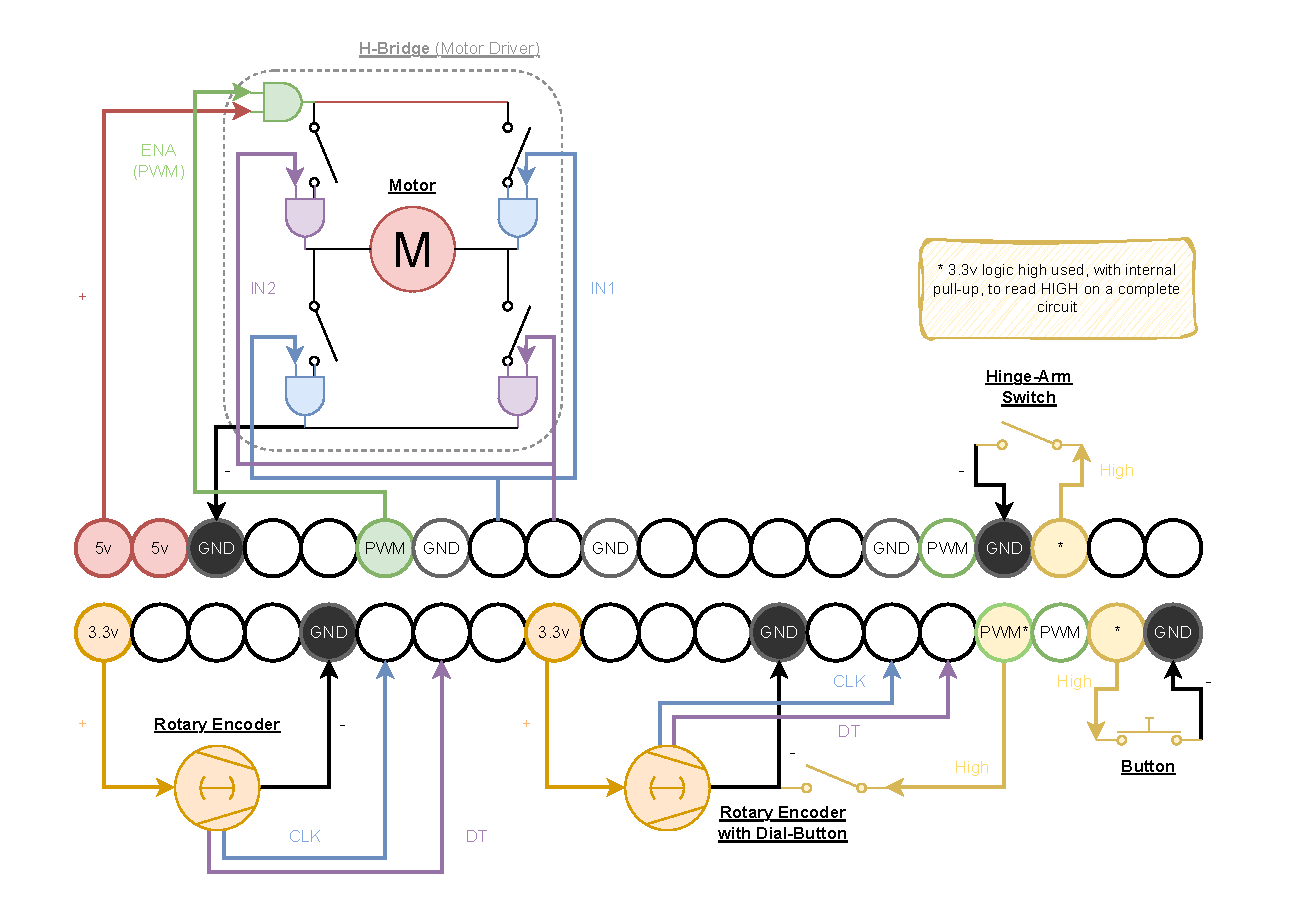
\includegraphics[width=0.5\linewidth]{images/CircuitDiagram.jpg}
                \caption{Circuit diagram of the connected components (TEMP! TODO: FORMALSIE)}
                \label{fig:circuitDiagram}
            \end{figure}
        
            \subsubsection{Challenges Encountered}
    
                During the implementation phase of the project, a few problems were encountered when handling the hardware components.
    
                \paragraph{'Measure Twice, Cut Once'}
    
                    Often, when developing software solution, it is common to use a 'trial and error' approach to make a system work. Whilst development is not a mindless task, developers will often just tweak small changes and run the system until it performs correctly, rather than fully designing every single aspect on paper first. For software, in development environments, this is safe to do and even works well as a time-efficient practice. Many technology stacks even accommodate this, with features such as hot-reloading.
    
                    However, when dealing with hardware, this is not the case. During the development of this product there were a few cases where irreparable damage was done to some components due to the use of the above software debugging technique. Whilst configuring the motor to support PWM, the motor driver's jumper connection (which connected the PWM EN input pin to the 5V pin for constant pulse) had to be removed, to allow the PWM GPIO pin to connect. However, after removing the jumper both pins were exposed, and rather than check which one was the correct pin, a rather careless attitude was taken, just guessing which pin it was. This resulted connecting the 3V PWM GPIO pin to a live 5V current, which fried the GPIO output.
    
                    Thankfully, the damaged pin was one of two which supports PWM on the RPi 5 model, and so, the backup pin was used.
    
                    However, this led to much more caution being used when handling the hardware components afterwards.
    
                \paragraph{Voltage Consumption}
    
                    During early development with the Pi, an unofficial charging cable was used as a power source whilst waiting for the official one to arrive. This cable did not have sufficient wattage for the Pi's specs, and, as a result, it was unable to power the device at high-load without causing the device to turn off.
    
                    To prevent this from being a total blocker, the device was configured to under-clock CPU usage, and some other things, in order to minimise the voltage draw of the device, to minimise how often this would occur.
    
                \paragraph{Overheating}
    
                    Sometimes, during long periods of development, the device would reach very high temperatures. Due to the RPi 5's increased specs over previous models, this is fairly common when running it even for small tasks with only active cooling. This began to throttle performance during long periods of development and/or testing, however, the solution was simply to setup an active cooling solution. Thankfully, the pins for controlling fan PWM based off of CPU temperatures are separate from the standard GPIO pins, and so did not affect any of the other components.
    
            \subsubsection*{Reflection}
                Hardware prototyping introduced physical risks absent in software — a fried GPIO pin taught caution the hard way. Pin planning and thermal issues were underestimated early on, but later handled with low-cost fixes and better care.
    
      \subsection{Machine Learning Model} \label{sec:mlImp}
    
            This section outlines the ML models used to classify album artwork, from early CNN prototypes to fine-tuned transfer learning pipelines. The evolution of model architecture, training experiments, and challenges are discussed.
    
            This section covers:
            \begin{itemize}
              \item Initial development using custom CNN models (Baby Ouroboros)
              \item Transition to transfer learning with ResNet18 (Ouroboros)
              \item Experiments with data augmentation and hyperparameter tuning
              \item Two extended architectures: Amphisbaena (multi-head) and Hydra (expandable)
              \item Training constraints and documentation efforts
            \end{itemize}
    
            \paragraph{Tooling and Training Setup}
    
            For implementation of the ML models, PyTorch was chosen over other libraries (such as TensorFlow, Keras, etc.) due to its superior debugging capabilities and flexibility. Given that this project focused on experimentation rather than production-grade deployment, PyTorch's dynamic computation graph and intuitive design made it a more suitable choice. Experimentation was done through Jupyter notebooks, which aided development due to easily allowing specific code snippets to re-run, and rendering results in-line.
    
            The initial goal was to create a full pipeline that could reasonably run on the Raspberry Pi model. Although, it was known that if the dataset grew beyond a toy sample size, whilst it would be possible to train using the Pi, it would not be efficient. With this in mind, all model training and experimentation was done on desktop computer, utilising an NVIDIA RTX 3060 Ti GPU. Eventually, the idea of running the model on the Pi was dropped entirely, however, it is still technically possible, it is just not reasonable for anything other than very small models (TODO- compare results and training times of RTX vsa Pi).
    
            \subsubsection{Model Development}
            
            \paragraph{Simple CNN: Baby Ouroboros Model}
    
                In keeping with the experimental learning-through-development approach, the most basic possible CNN model was initially created, as shown in Figure~\ref{fig:BabyOuroboros}. The architecture for this was largely informed by TODO, and the first implementation was referred to as SimpleCNN.
    
                \begin{figure}[htbp]
                    \centering
                    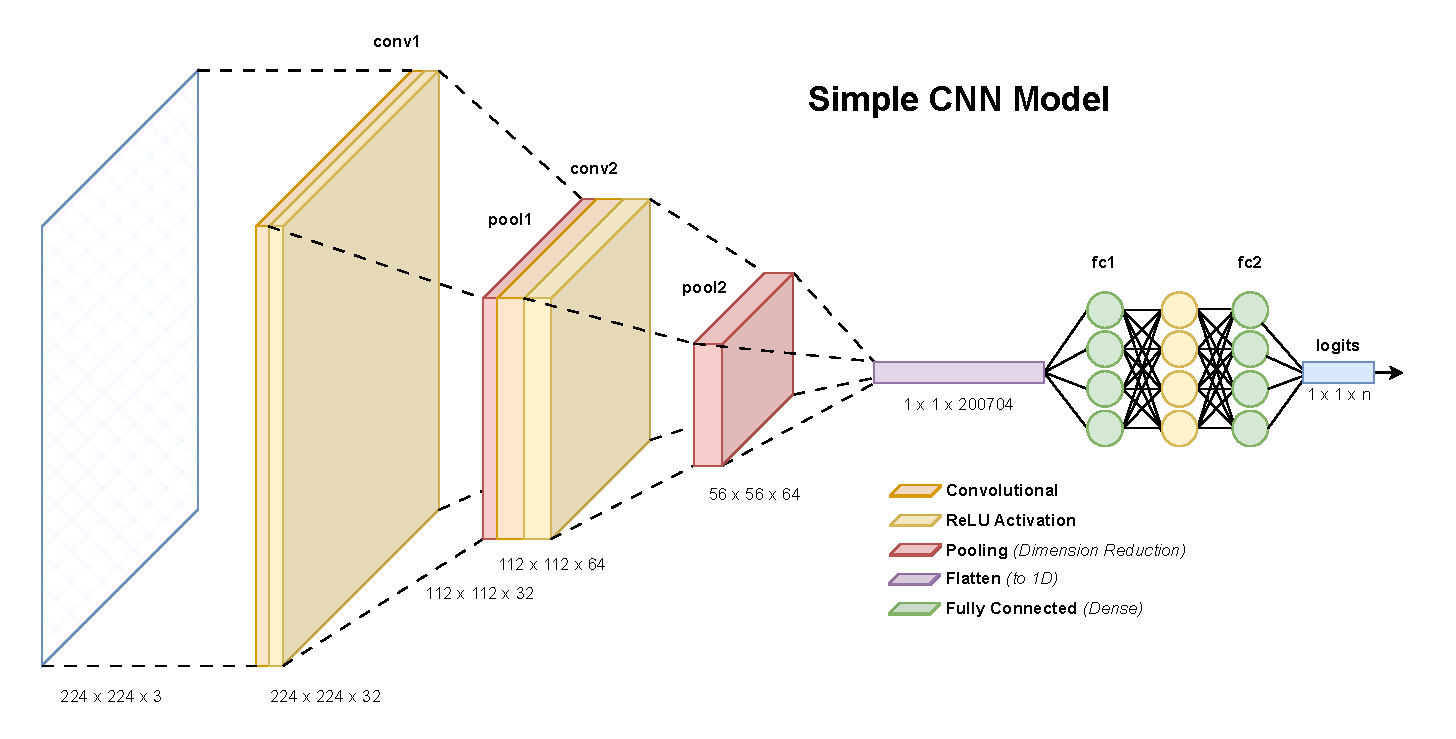
\includegraphics[width=\linewidth]{images/BabyOuroboros.pdf}
                    \caption{Architecture for simple CNN model}
                    \label{fig:BabyOuroboros}
                \end{figure}
    
                The first iteration of this model (SimpleCNN 'Mini') was trained on only the exceptionally small TODO dataset, as a proof of concept. Figure~\ref{fig:SimpleCNN-Mini_Train} shows how the models accuracy increased as training progressed. Whilst the model rather quickly converged and showed good results on the training data (eventually overfitting), the validation dataset's accuracy did climb in slow intervals, but never exceeded 60\%. Whilst this was a good start, it was thought that the problem with this poor generalisation likely came from the sheer small scale of the dataset.
    
                All input data was normalised according to the same dataset statistic:
                    \[
                    x' = \frac{x - \mu}{\sigma}
                    \]
                where:
                    \begin{itemize}
                        \item \( \mu \) is the mean pixel value \([R,G,B]\) of the dataset.
                        \item \( \sigma \) is the standard deviation of the pixel values.
                    \end{itemize}
    
                Initially, this was calculated as a channel-wide measure of the full combined dataset. However, the standardised ImageNet distribution was also used, with \( \mu = [0.485, 0.456, 0.406] \) and \( \sigma = [0.229, 0.224, 0.225] \), to leverage the greater variation of images it has. Figure~\ref{fig:normalisedArts} shows an example batch of images, normalised to the ImageNet standard.
        
                \begin{figure}[h]
                    \centering
                    
\includegraphics[width=\textwidth]{images/NormalisedArts.png}
                    \caption{Example of normalised dataset batch.}
                    \label{fig:normalisedArts}
                    \caption*{
                        Original artworks are © their respective copyright owners
                        \footnotesize These images have been processed for research/educational purposes and do not intend to infringe upon the original copyrights.
                    }
                \end{figure}
    
                Conforming the data to an external distribution can be a good practice for consistency and compatibility, particularly if there was a chance of later using transfer learning or pre-trained models.
    
                \begin{figure}[h]
                    \centering
                    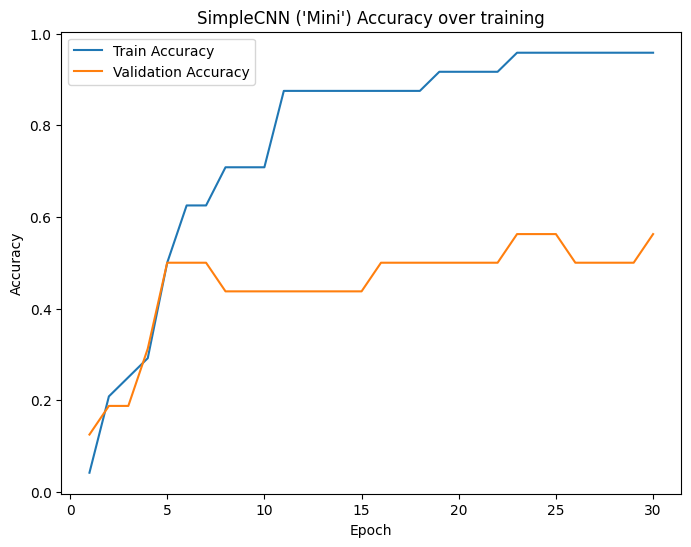
\includegraphics[width=\textwidth]{images/SimpleCNN-Mini_Train.png}
                    \caption{Accuracies of simple CNN architecture on small dataset, per epoch.}
                    \label{fig:SimpleCNN-Mini_Train}
                    \caption*{Higher is better. Training of a SimpleCNN model on \ref{data:mini}; validated against \ref{data:val}.}
                \end{figure}
    
                The same model architecture was then used to train on a much a larger dataset (TODO). However, this model performed horrendously with the sudden increase of data. As shown in Figure~\ref{fig:SimpleCNNs_TrainLoss-Mini_Train} whilst the loss (distance of predictions from the true results) decreases rather smoothly on the smaller dataset, when trying to learn from TODO, the model very sharply overfits, and actually worsened in validation performance, never even improving beyond the smaller dataset's initial performance. Figure~\ref{fig:SimpleCNNs_PeakAccuracy-Mini_Train} shows the differences of the best-observed performances of this model architecture across these two training scenarios, showing that performance decreased as the dataset increased.
        
                \begin{figure}[h]
                    \centering
                    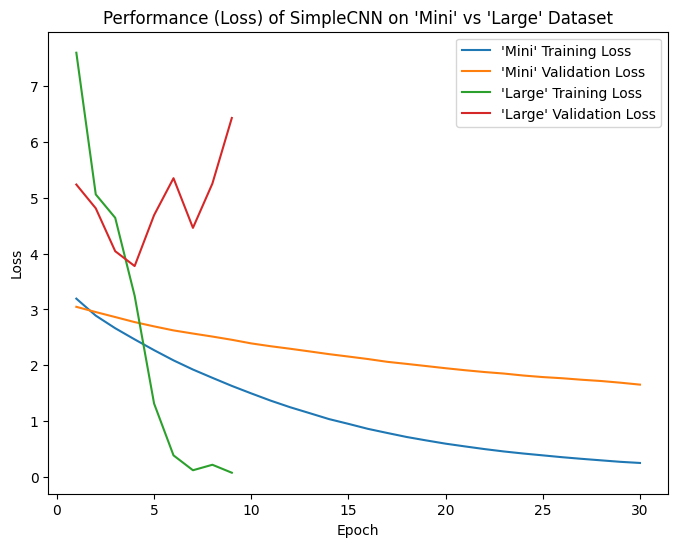
\includegraphics[width=\textwidth]{images/SimpleCNNs_TrainLoss.png}
                    \caption{Comparison of SimpleCNN architecture performance on different sized datasets}
                    \label{fig:SimpleCNNs_TrainLoss-Mini_Train}
                    \caption*{Lower is better. Trained on 'Mini' (\ref{data:mini}) and 'Large' (\ref{data:large}) datasets; both validated against \ref{data:val}.}
                \end{figure}
        
                \begin{figure}[h]
                    \centering
                    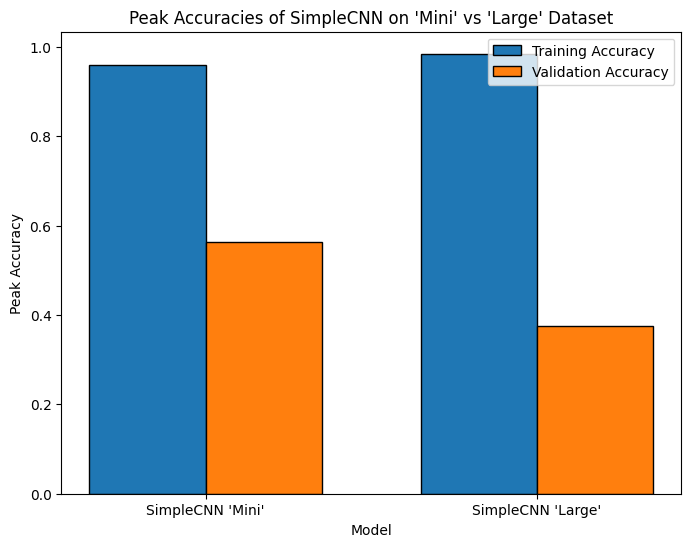
\includegraphics[width=\textwidth]{images/SimpleCNNs_PeakAccuracy.png}
                    \caption{Comparison of best-case SimpleCNN performance on different sized datasets}
                    \label{fig:SimpleCNNs_PeakAccuracy-Mini_Train}
                    \caption*{Trained on 'Mini' (\ref{data:mini}) and 'Large' (\ref{data:large}) datasets; both validated against \ref{data:val}.}
                \end{figure}
    
                This model performed reasonably on small datasets, but could not scale, and so was labelled as Baby Ouroboros.
    
                In order to improve the results for the large dataset, a deeper model would be required. Various experiments were done with various configurations and depths of model (broadly named DeepCNN), however, as the range of albums had increased, even with a greater depth, the feature extraction mechanisms seemed to be lacking. As networks become deeper they require exponentially more data in order to learn sufficiently.
    
                \paragraph{Transfer Learning: Ouroboros Model}
    
                After the results of the deeper versions of Baby Ouroboros did not prove very fruitful, a new architecture was planned. Rather than trying to train a model from scratch, it was decided to trial using a feature-extractor from an existing model, which had been trained on a much larger and more generalised dataset. In order to do this, the ResNet18 model selected, which has been trained on the immense ImageNet library. In theory, a custom solution could have still been trained using this publicly available dataset, with the published parameters and architecture of these models, however, for faster development iterations, it was decided to use a pre-trained feature-extractor, and to either fine-tune it, or just build a classifier system on top of it.
    
                The ResNet18 model, by itself has a powerful feature extractor, however just appending a classifier head on top would yield purely random results, if not further refined through specialised training for the album-recognition task.
    
                \subsubsection{Training Experiments}
    
                    Initially, all ResNet18 weights were frozen, with only the appended classifier head being trained. This approach was intended to avoid heavy biasing and retain pre-trained knowledge, and it already outperformed the in-house DeepCNN model. Further experiments involved selectively unfreezing and fine-tuning varying numbers of layers from the base model to inspect the affect this had on performance.
    
                    \begin{figure}
                        \centering
                        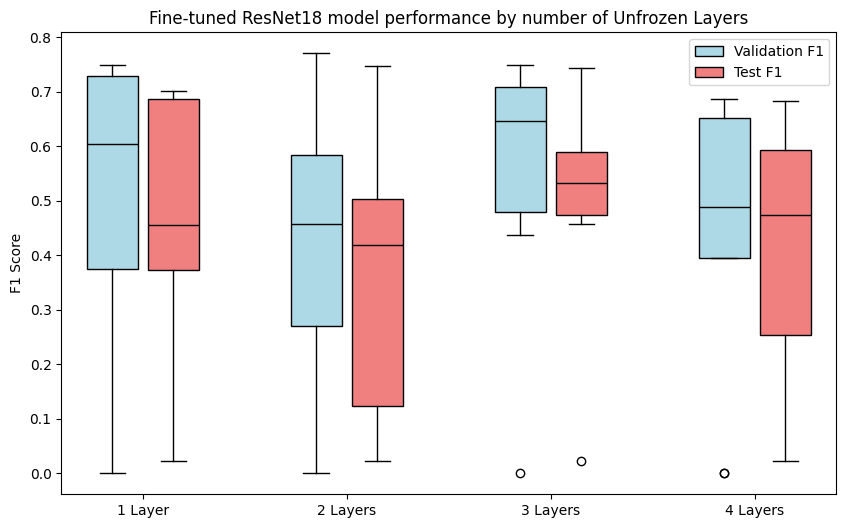
\includegraphics[width=\textwidth]{images/ResNetLayerTests.png}
                        \caption{Boxplot showing the distribution of F1 scores across training epochs for different numbers of unfrozen layers in a fine-tuned ResNet18.} \label{fig:ResNetLayers}
                    \end{figure}
                    
                    As shown in Figure~\ref{fig:ResNetLayers}, the highest validation and test scores were achieved when fine-tuning two layers of the base model. This configuration was therefore preferred in most tests. However, while the 2-layer setup yielded the highest peak results, it also exhibited a broad and low-spread distribution across training epochs. This highlights the importance of choosing the right number of training epochs: stopping too early or training for too long can significantly degrade performance, and so particular care had to be taken in other experimental scenarios using this configuration, to ensure that epoch count was not the deciding factor influencing results.
        
                    \paragraph{Hyperparameter Search}
        
                        A large-scale hyper-parameter grid search was conducted, training the model over various different combinations of value for certain aspects: learning rate, weight decay, number on unfrozen layers, batch size, etc. The results of one test, evaluating different learning rates and weight decays, over each training cycle (epoch), can been seen in Figure~\ref{fig:ResNet_AugGrid}, with the best observed accuracies shown in Figure~\ref{fig:ResNet_AugGridHist}.
                
                        \begin{figure}[h]
                            \centering
                            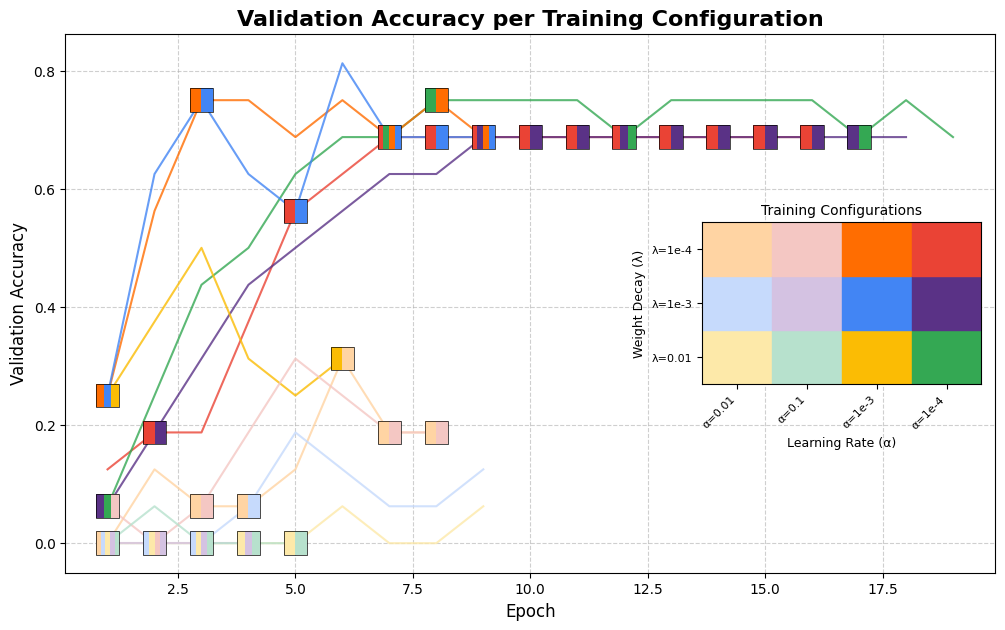
\includegraphics[width=\textwidth]{images/ResNetCNN_AugGrid.png}
                            \caption{Performance results of ResNet18 fine-tuned model hyperparamter grid search}
                            \caption*{Performed on \ref{data:aug} training set (1,176 images) with batch size of 8; validated against \ref{data:val}. Early stopping used when validation loss degraded, so not all configurations ran for equal epochs. Where multiple configurations have the same performance at the same epoch, a square marker indicates which colours are represented.}
                            \label{fig:ResNet_AugGrid}
                        \end{figure}
                
                        \begin{figure}[h]
                            \centering
                            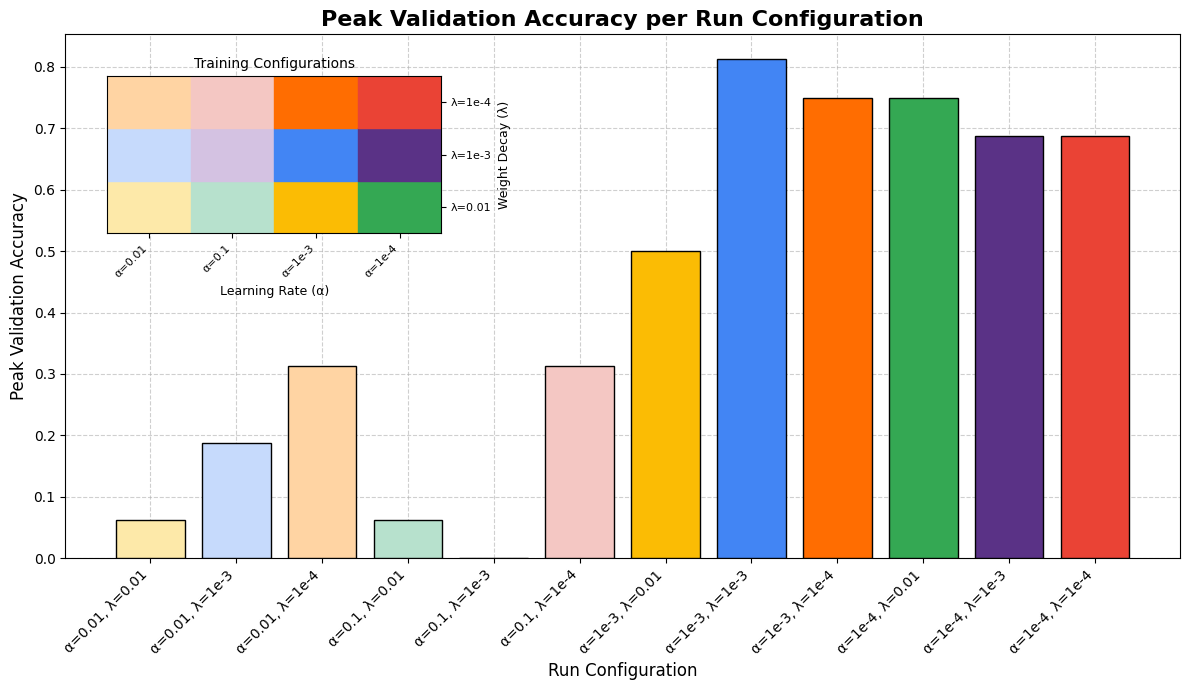
\includegraphics[width=\textwidth]{images/ResNetCNN_AugGridHist.png}
                            \caption{Best-case performance results of ResNet18 fine-tuned model hyperparamter grid search}
                            \caption*{
                                Full set of accuracies during training can be seen in Figure~\ref{fig:ResNet_AugGrid}.
                            }
                            \label{fig:ResNet_AugGridHist}
                        \end{figure}
        
                    \paragraph{Data Augmentation}
        
                        In addition to experimenting with the model's configuration, the data was also investigated. Since the design phase, it was known that this model would likely not need much generalisation techniques, due to being a closed-world task, however, to make the model as robust as possible, data augmentation was still investigated. In a real use case, even though the images will be very similar to their training data, there could be slight fluctuations in rotation, size, and lighting or fading of the artwork. Additionally, some extreme transformations might occur, such as the artwork being fully upside down. In order to make the system handle this, each epoch of training was bolstered with augmented copies of with artificial transformations, de-colourings, and cropping taking place (see Figure~\ref{fig:augmentedArts} for an example).
    
                        \begin{figure}[h]
                            \centering
                            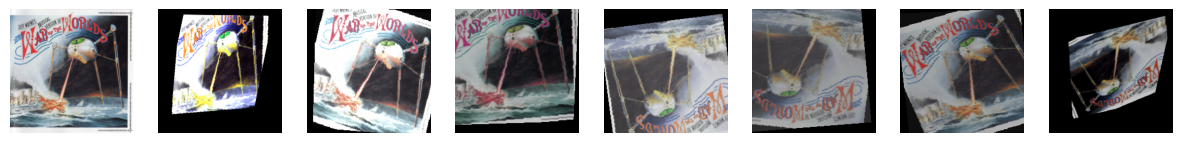
\includegraphics[width=\textwidth]{images/AugmentedArts.png}
                            \caption{Example of augmented dataset batch (without normalisation).}
                            \label{fig:augmentedArts}
                            \caption*{
                                The first image is the unaltered original, whereas the rest of the batch have all be augmented over their rotation, size, cropping, colour, affinity and perspective.
                            }
                            \caption*{
                                Album artwork from \textit{Jeff Wayne's Musical Version of The War of the Worlds} (1978).  
                                \footnotesize Used for research/educational purposes. All rights remain with the original copyright holders.
                            }
                        \end{figure}
    
                        This augmentation was generated 'on-the-fly' during training, meaning no modified image was saved or stored beyond the training epoch. Additionally, this meant that each epoch had slightly different variations it was learning on. This made the training process better for generalisation, serving as a forced dropout of seen images; however, the training process became slower, requiring more training epochs to accurately learn from the data, as well as the dataset now be scaled to be a factor bigger, increasing the time taken to train.
    
                        Even with GPU optimisation, as the dataset multiplied in size, it became to hold to store within the available VRAM at once, and so batch sizes had to be decreased from ~32 to ~8, in most cases, further slowing the training process.
    
                        This 'on-the-fly' approach also had drawbacks, as it required additional rendering computations in every epoch cycle, however, the performance gains made the extra time taken a worthwhile trade-off.
        
                    \paragraph{Data Hyperparamaters}
    
                        Not only was the model configuration rigorously tested under various alterations, but also the training dataset.
    
                        One notable requirement of a CNN model, is that all input data must be the same size, that is, the images must all be of uniform dimensions. The initial baseline used was 244x244, however it was theorised that greater fidelity versions of images could improve quality.
    
                        As per Figure~\ref{fig:CNNSize_Perf}, various image sizes were tested in the TODO model, to varying degrees of observed success. Whilst the 124x124 size did have the highest peak in performance, the 244x244 was most consisent in its performance. The more extreme sizes seemed to perform most poorly, likely due to the smallest images having too great of a loss in details to be learnable, whereas the larger images were likely subject to too much noise and variation, as well as potentially requiring more epochs or a deeper network with larger convolution kernels to adequately learn details.
            
                        \begin{figure}[h]
                            \centering
                            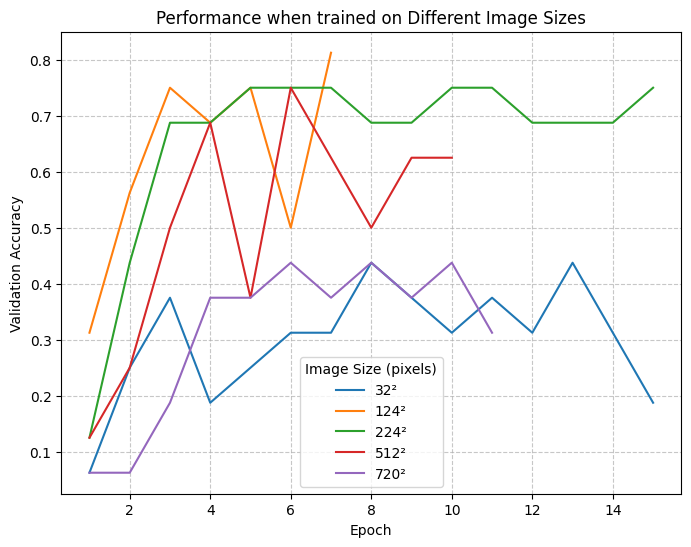
\includegraphics[width=\textwidth]{images/CNNSize_Perf.png}
                            \caption{Model accuracy per training epoch, using different image sizes}
                            \label{fig:CNNSize_Perf}
                            \caption*{Results are averaged over multiple attempts.}
                        \end{figure}
    
                        The 124x124, 244x244, and 512x512 configurations were further experimented with, however, as per Figure~\ref{fig:CNNSize_Time}, training time scaled roughly quadratically as the area of the image increased, an expected result seeing as convolution is highly dependent on per-pixel processes (even when done in batches, via matrix representations). For this reason, 244x244 was selected as the primary image size, due to having the most consistent performance with very small time constraints compared to the smaller 124x124 form factor.
    
                        Additionally, when switching to utilise the ResNet feature extractor, the 244x244 was especially the best-performing, as this was the input size used for the model's initial training.
                
                        \begin{figure}[h]
                            \centering
                            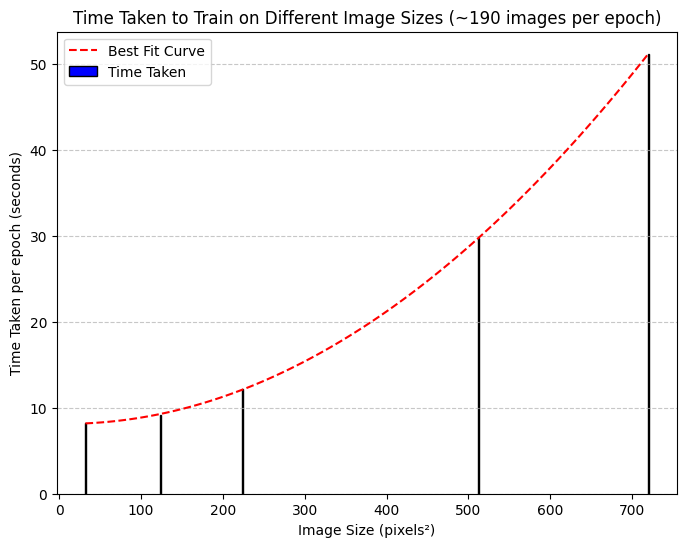
\includegraphics[width=\textwidth]{images/CNNSize_Time.png}
                            \caption{Average training time for different image sizes}
                            \label{fig:CNNSize_Time}
                            \caption*{Results are averaged over multiple attempts.}
                        \end{figure}
    
            \subsubsection{Extended Architectures}
    
                \paragraph{Amphisbaena (Multi-Headed)}
    
                The Ouroboros model, using the ResNet18 architecture, was additionally built upon to have two classification heads, allowing the model to learn different categories for the same items. In addition to learning the album, this allowed learning a de-coupled artist value. Using a single network, diverging into two output heads at the end allowed for shared learning from feature extraction, and reduced redundant duplication of resource-heavy processes (for example, this task could be done with two fully separate models, but would double the training time).
    
                \begin{temp}
                    Multi-Head Model Diagram
                \end{temp}
    
                This was largely done as an experimental feature, as it was unknown how well an artist can be detected, on unseen data, from other albums of the same artist. Whilst author classification is an area being explored for visual artists, this is a much more generalised task for album covers, as two albums by the same musician may feature two drastically different artworks produced by different artists, with little-to-no overlap. However, some musicians do have stylistic consistency in their albums covers. A notable example in pop culture is Ed Sheeran, whose albums often feature mathematical symbols and paint effects (see Appendix~\ref{app:Cult}, Figure~\ref{fig:EdMeme} for a comedic example). Additionally, albums by the same musician may consistently feature a logo, brand, or even the their likeness, which could be enough information for a deep model to learn from. And, finally, many album arts are done by the same artist for a single performer or band, and so even stylistic aspects could still be beneficial.
    
                \begin{figure}[h]
                    \centering
                    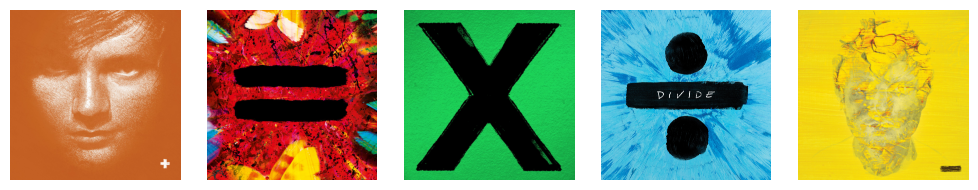
\includegraphics[width=0.6\textwidth]{images/EdAlbums.png}
                    \caption{Album covers of Ed Sheeran’s studio albums}
                    \label{fig:EdAlbums}
                    \caption*{+ (2011), = (2021), × (2014), ÷ (2017), and − (2023). \\ Images © Asylum Records / Atlantic Records. Retrieved from Cover Art Archive.}
                \end{figure}
    
                After some experimentation, it was found that the model was able to achieve some level of success. As a proof of concept, as part of the TODO dataset, four of Ed Sheeran's albums were included. These images (the first four, from the left, in Figure~\ref{fig:EdAlbums}) were able to learn enough information such that the − (2023) album (right-most image) was able to be correctly identified as an Ed Sheeran album (64\% confidence).
    
                It is worth noting that this use case is a particularly ideal one, however, with Ed Sheeran's album all being very uniformly consistent.
    
                The aim to experiment with additional channels as classification, such as genre of decade, was ultimately not viable within the time, alongside the rest of development, and so were left.
    
                \paragraph{Hydra (Expandable)}
    
                The creation of the dynamically-expandable classification system was conducted, however, due to time constraints only minimal experimentation was conducted. The use-case for this model was that, if a user had a large collection and had set up this system to classify them, but then bought a new record, they would have to fully re-train a new model from scratch, to accommodate the new addition. Furthermore, if the model was performing poorly on some albums, the user would, theoretically, be able to inform the system of this, essentially acting as a manual annotator, which could be used to give higher weightings to these albums, to tune the model to match user expectations. This goal of high-level model customisation was challenging, however.
    
                At first, the idea was to simply fine-tune the previously trained models, using a new collection of data. However, it was quickly found that catastrophic data loss occurred when altering weights without the original training images to validate them.
    
                In order to avoid the retention or re-downloading of copyrighted images to be required for this system to work, instead a matrix database was created. The classification model essentially has two components: a feature extractor and a classifier. The idea was to, once initial training was complete, run each training image through the feature-extractor only, and to store the numerical tensor (the embedding) in this database. Then, if a future revision of the model was desired, the feature extractor could be frozen, then classifier could be re-initialised to allow an additional album, and the already-extracted features could be fed directly into the classifier, alongside the new data going through the full model, to ensure training saw both sets of data.
    
                Whilst this technique showed better results, it was still prone to catastrophic data loss, either biasing towards the new data, or the original data. Freezing the feature extractor, whilst allowing to remember old features better, prevented the model from being able to correctly learn new albums; however, removing this constraint resulted in the previously extracted data sometimes being almost-random in accuracy-- sometimes performing okay, but other times not; with no consistent way of ensuring ideal performance.
    
                For this, a PNN architecture was created, allowing a dynamic number of heads to operate in parallel, using a weighted consensus approach to generate a single classification. This idea still utilised a single, frozen feature extractor, utilising the retained embeddings, however, rather than replacing the classifier, a new classifier was added in tandem to the original one. Then, during training, the two heads were weighted, through cross-entropy loss, so that the final result was the 'consensus' of the two. Essentially, the original model was preferred, unless the second model had a high degree of confidence that it was a new class, in which case, the system delegated to the newer head if, and only if, the original head was not also highly confident.
    
                This system showed promising improvement over the early attempts, however performance degradation was still significant, with the model dropping from \~80\% confidence on the initial images to \~30\% (though, accuracy was maintained in the very small testing sample set used). This showed that the dynamic approach was at least, potentially,  viable for a full-scale solution. However, due to time constraints, no further experimentation was done on this concept.
    
                A major issue with the initial vision, however, was that if a user wanted to update their model, this training system would ideally need to be run on-demand on the Pi. Due to the need of the vector database, and a deep model, for the results acquired, this means that the training process would be significantly slow, on the SBC, and therefore, might have to be done as a once-per-day system, as a limitation of the hardware.
    
            \subsubsection{Documentation}
    
                Additionally, in order to make the models clear and distinct from one another, as well as being potentially useful to other developers, a model card \cite{Mitchell_2019} was created, for each.
            
            \subsubsection{Challenges Encountered}
    
                On the 8th of October 2024, the Internet Archive experienced a significant cyberattack that led to a temporary outage of its services, including the Cover Art Archive. The breach exposed data from approximately 31 million user accounts, revealing email addresses, screen names, and bcrypt-hashed passwords. %https://www.forbes.com/sites/larsdaniel/2024/10/20/internet-archive-breached-again-third-cyber-attack-in-october-2024/
    
                This posed a fairly significant issue for the project, as the Cover Art Archive had been selected as the source of the training datasets, however, as a joint project between the Internet Archive and MusicBrainz, was among the affected services. Users reported issues accessing cover art images during the outage. %https://community.metabrainz.org/t/internet-archive-down-possibly-hacked/718418
    
                This outage lasted for weeks, with components being brought back online one-by-one,
                %https://blog.archive.org/2024/10/21/internet-archive-services-update-2024-10-21/
                with the Cover Art Archive not being restored until after the 21st. Fortunately, a small 'toy' scale dataset had already been accumulated, in addition to the physically-owned copies that could be used, and so this did not become too much of an issue for the project. Whilst model training was limited to small-scale models, these weeks were used mostly on development of the web components.
    
                If, however, this outage had continued for longer, then serious consideration of finding a new service would have been required. During these weeks, additional research into such systems was done, an Last.fm was selected as a backup. But, once the Cover Art Archive was restored, no further issues occurred during development, regarding data availability. Although, more outages of the service have been reported, post-development. % https://hackread.com/internet-archive-archive-org-down-power-outage/
    
            \subsubsection*{Reflection}
                The early CNNs underperformed at scale, but transfer learning delivered strong results with less training overhead. Attempts at less redundant systems (Amphisbaena) and dynamic expansion (Hydra) were promising, though not production-ready — future work could refine this into a truly user-adaptive system.
    
    %%%%%%%%%%%%%%%%%% SECTION 5 %%%%%%%%%%%%%%%%%%
    \section{Results} % edit section heading as appropriate
        % results of soft/hardware testing
        % screenshots of UI / program output
    
        This section presents the completed outputs of the system: a functional full-stack application, an interactive hardware artefact, and their seamless integration into a hybrid user experience. It provides a visual and descriptive overview of each element, highlighting what was achieved and what functionality is offered to the end user.
        
        Detailed evaluation of their effectiveness, usability, and alignment with the project aims is presented in Section~\ref{sec:evaluation}.
        
        \subsection{Software Artefact}
    
            The system includes a complete browser-based application designed for playback control, visual feedback, and media interaction. It supports both a local host interface (projected onto the device) and external client interfaces (via mobile or desktop browsers), all communicating with a central backend.
    
            \paragraph{Host Interface}
    
            The host interface runs on the local device and is the main control centre of the system. It provides visual feedback during playback. The UI is minimal by default, giving only the same information a physical vinyl on a player would: its centre label artwork; maintaining an unobtrusive appearance. Additional UI elements and controls remain hidden by default and only appear with active input (e.g., mouse movement), showing greater details (album art, album name, track name, etc.) and providing a digital method to achieve each use case (as per Figure~\ref{fig:umlusecase}).
    
            Figures~\ref{fig:hostQuiet}–\ref{fig:hostGui} show the host view with and without active UI overlays.
    
            \begin{figure}[h]
                \centering
                \begin{minipage}[b]{0.45\textwidth}
                    \centering
                    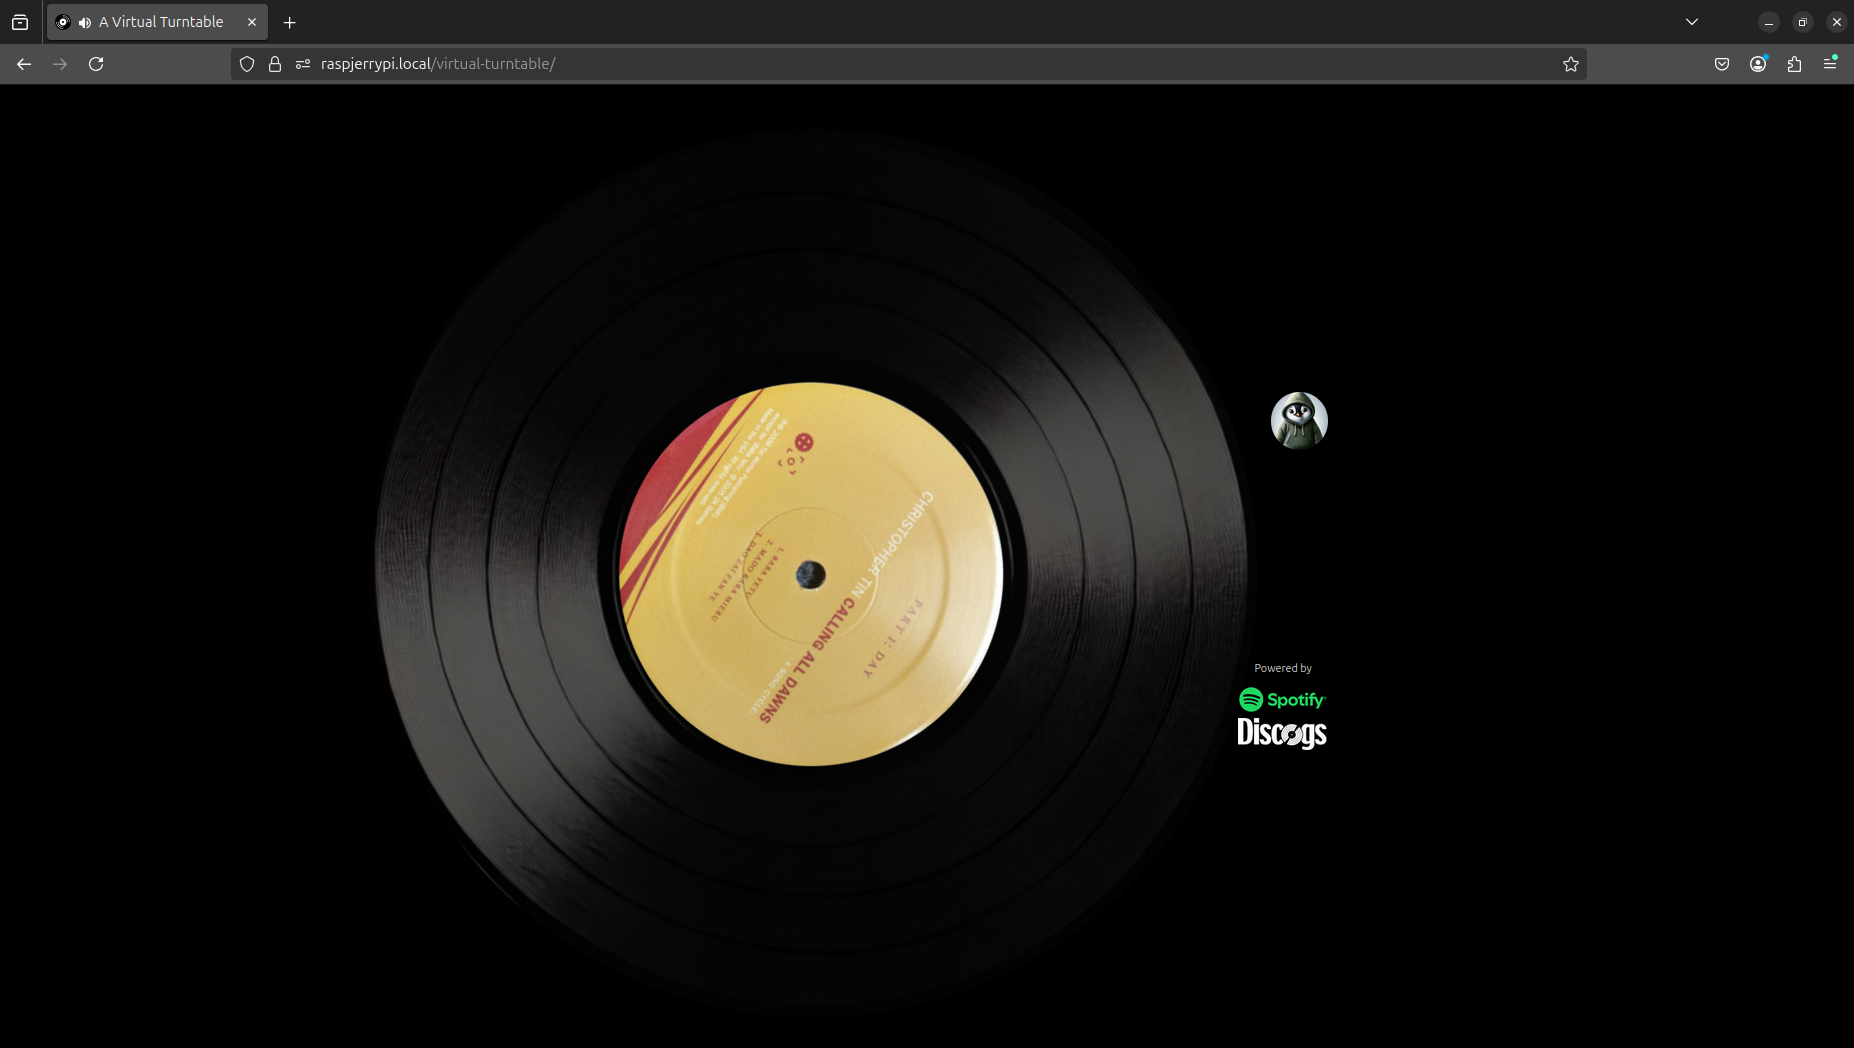
\includegraphics[width=\textwidth]{images/screenshots/HOST_Quiet.png}
                    \caption{Host client playing a track}
                    \label{fig:hostQuiet}
                \end{minipage}
                \hfill
                \begin{minipage}[b]{0.45\textwidth}
                    \centering
                    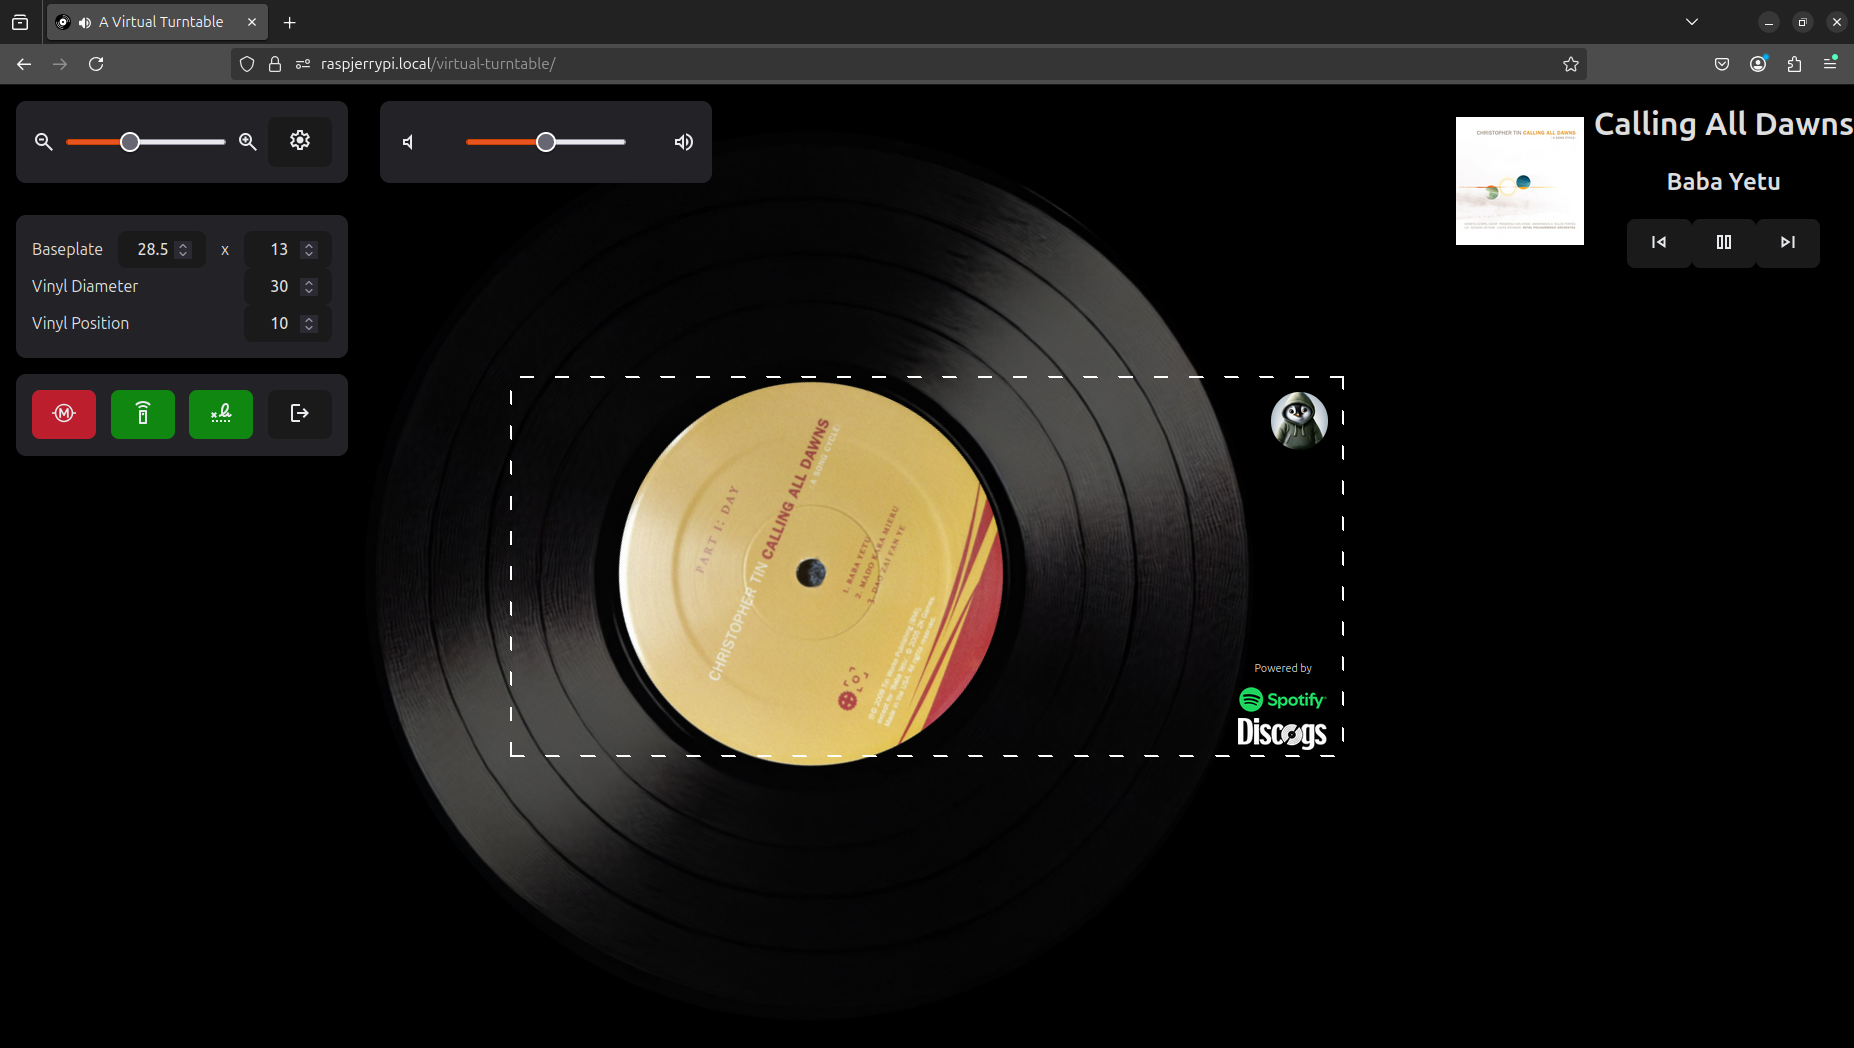
\includegraphics[width=\textwidth]{images/screenshots/HOST_GUI.png}
                    \caption{Host client playing a track, with UI overlays}
                    \label{fig:hostGui}
                \end{minipage}
            \end{figure}
    
            \paragraph{Remote Client Interface}
    
            The system also provides a web-based remote interface, enabling mobile phones or desktop browsers to connect over the local network. These clients replicate the core controls of the host -- such as play/pause, volume, track skip, and album scanning — allowing accessible, shared interaction. Figures~\ref{fig:laptop}–\ref{fig:phone} show examples of remote clients in use on different devices.
    
            \begin{figure}[h]
                \centering
                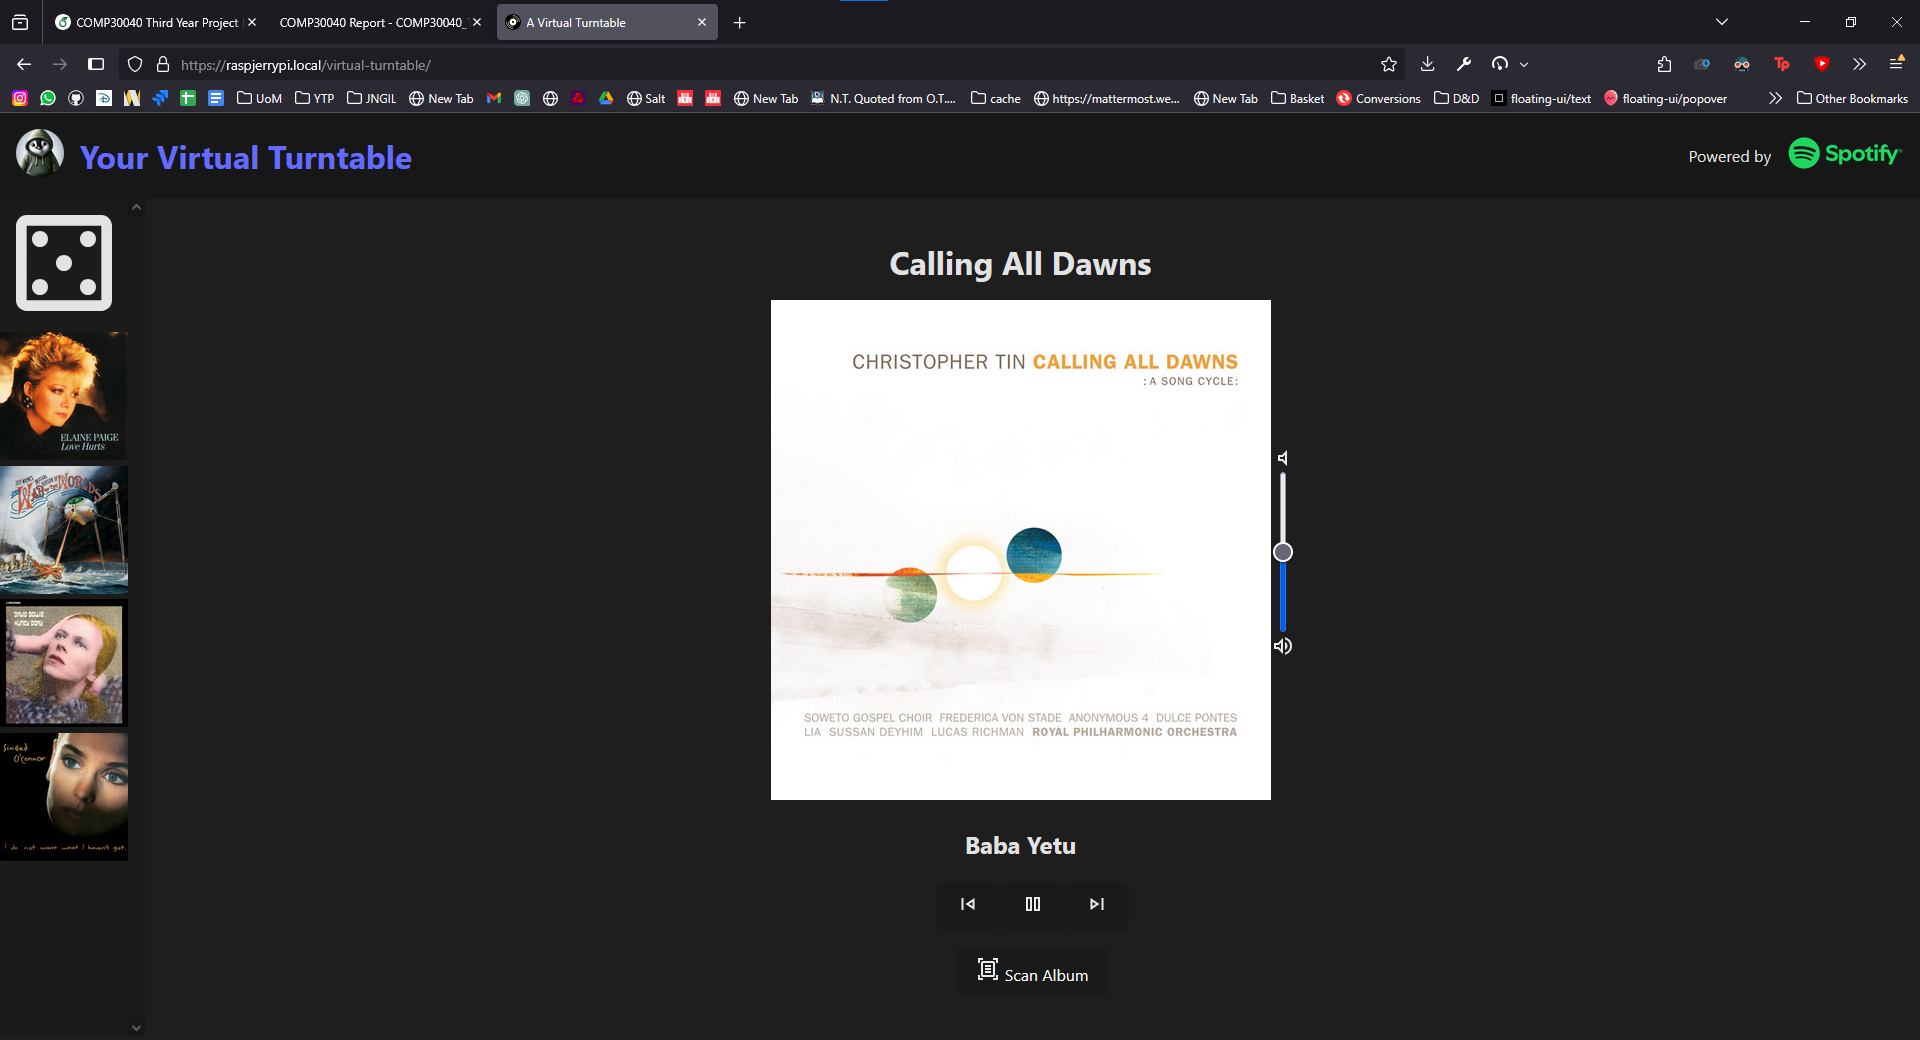
\includegraphics[width=0.4\textwidth]{images/screenshots/LAPTOP.png}
                \caption{Screenshot of a remote client (PC) connected to the host}
                \label{fig:laptop}
            \end{figure}
            
            \begin{figure}[h]
                \centering
                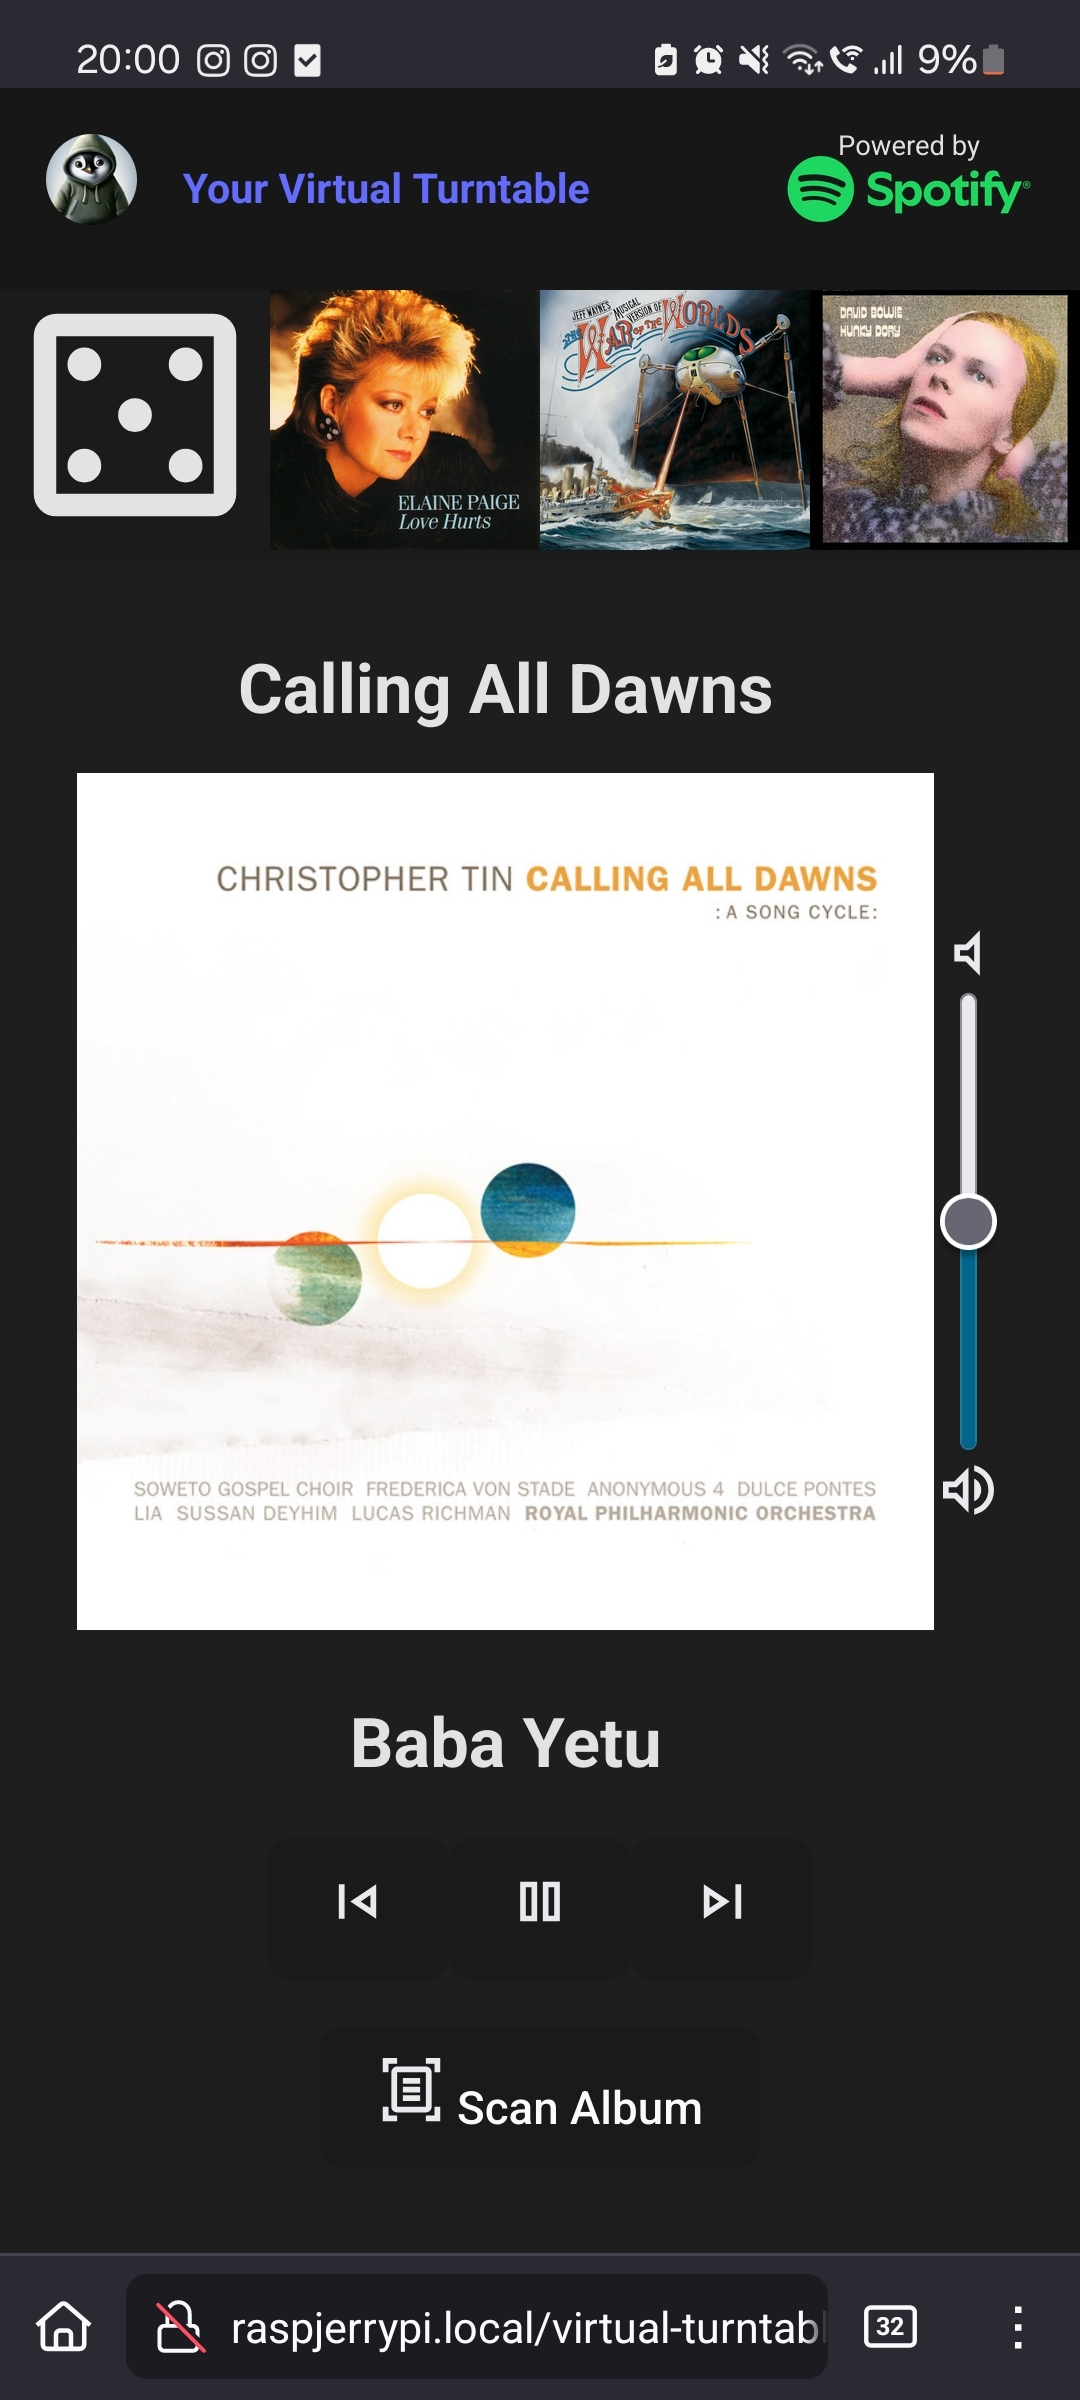
\includegraphics[width=0.4\textwidth]{images/screenshots/PHONE.jpg}
                \caption{Screenshot of a remote client (mobile) connected to the host}
                \label{fig:phone}
            \end{figure}
    
            \paragraph{Classification Model}
        
        \subsection{Hardware Artefact}
    
            The system is built into a physical Raspberry Pi-powered device. The unit includes tactile controls such as a rotary dial, physical button, and hinged `playback arm' -- each mapped to corresponding actions (e.g., play/pause, track skip, scan).
    
            A webcam is mounted to capture album cover images for recognition, and a motor spins a disc during playback, creating a dynamic and nostalgic effect. Figures~\ref{fig:product}–\ref{fig:bottom} show the unit from various perspectives, demonstrating form factor and component layout.
    
            \begin{figure}[H]
                \centering
                \begin{minipage}[b]{0.45\textwidth}
                    \centering
                    \includegraphics[width=\textwidth]{images/photos/product_1.jpg}
                \end{minipage}
                \hfill
                \begin{minipage}[b]{0.45\textwidth}
                    \centering
                    \includegraphics[width=\textwidth]{images/photos/product_2.jpg}
                \end{minipage}
                \caption{The finished build, with playback arm raised (left) and lowered (right).}
                \label{fig:product}
            \end{figure}
    
            \begin{figure}[H]
                \centering
                \begin{minipage}[b]{0.45\textwidth}
                    \centering
                    \includegraphics[width=\textwidth]{images/photos/profile_TOP.jpg}
                    \caption{Top-down profile of the device (circuitry exposed)}
                    \label{fig:top1}
                \end{minipage}
                \hfill
                \begin{minipage}[b]{0.45\textwidth}
                    \centering
                    \includegraphics[width=\textwidth]{images/photos/profile_TOP3.jpg}
                    \caption{Top-down profile of the device (with vinyl attached and  playback arm lowered)}
                    \label{fig:top2}
                \end{minipage}
            \end{figure}
    
            \begin{figure}[H]
                \centering
                \begin{minipage}[b]{0.45\textwidth}
                    \centering
                    \includegraphics[width=\textwidth]{images/photos/profile_FRONT.jpg}
                    \caption{Front profile of the device}
                    \label{fig:front}
                \end{minipage}
                \hfill
                \begin{minipage}[b]{0.45\textwidth}
                    \centering
                    \includegraphics[width=\textwidth]{images/photos/profile_BACK.jpg}
                    \caption{Back profile of the device}
                    \label{fig:back}
                \end{minipage}
            \end{figure}
    
            \begin{figure}[H]
                \centering
                \begin{minipage}[b]{0.225\textwidth}
                    \centering
                    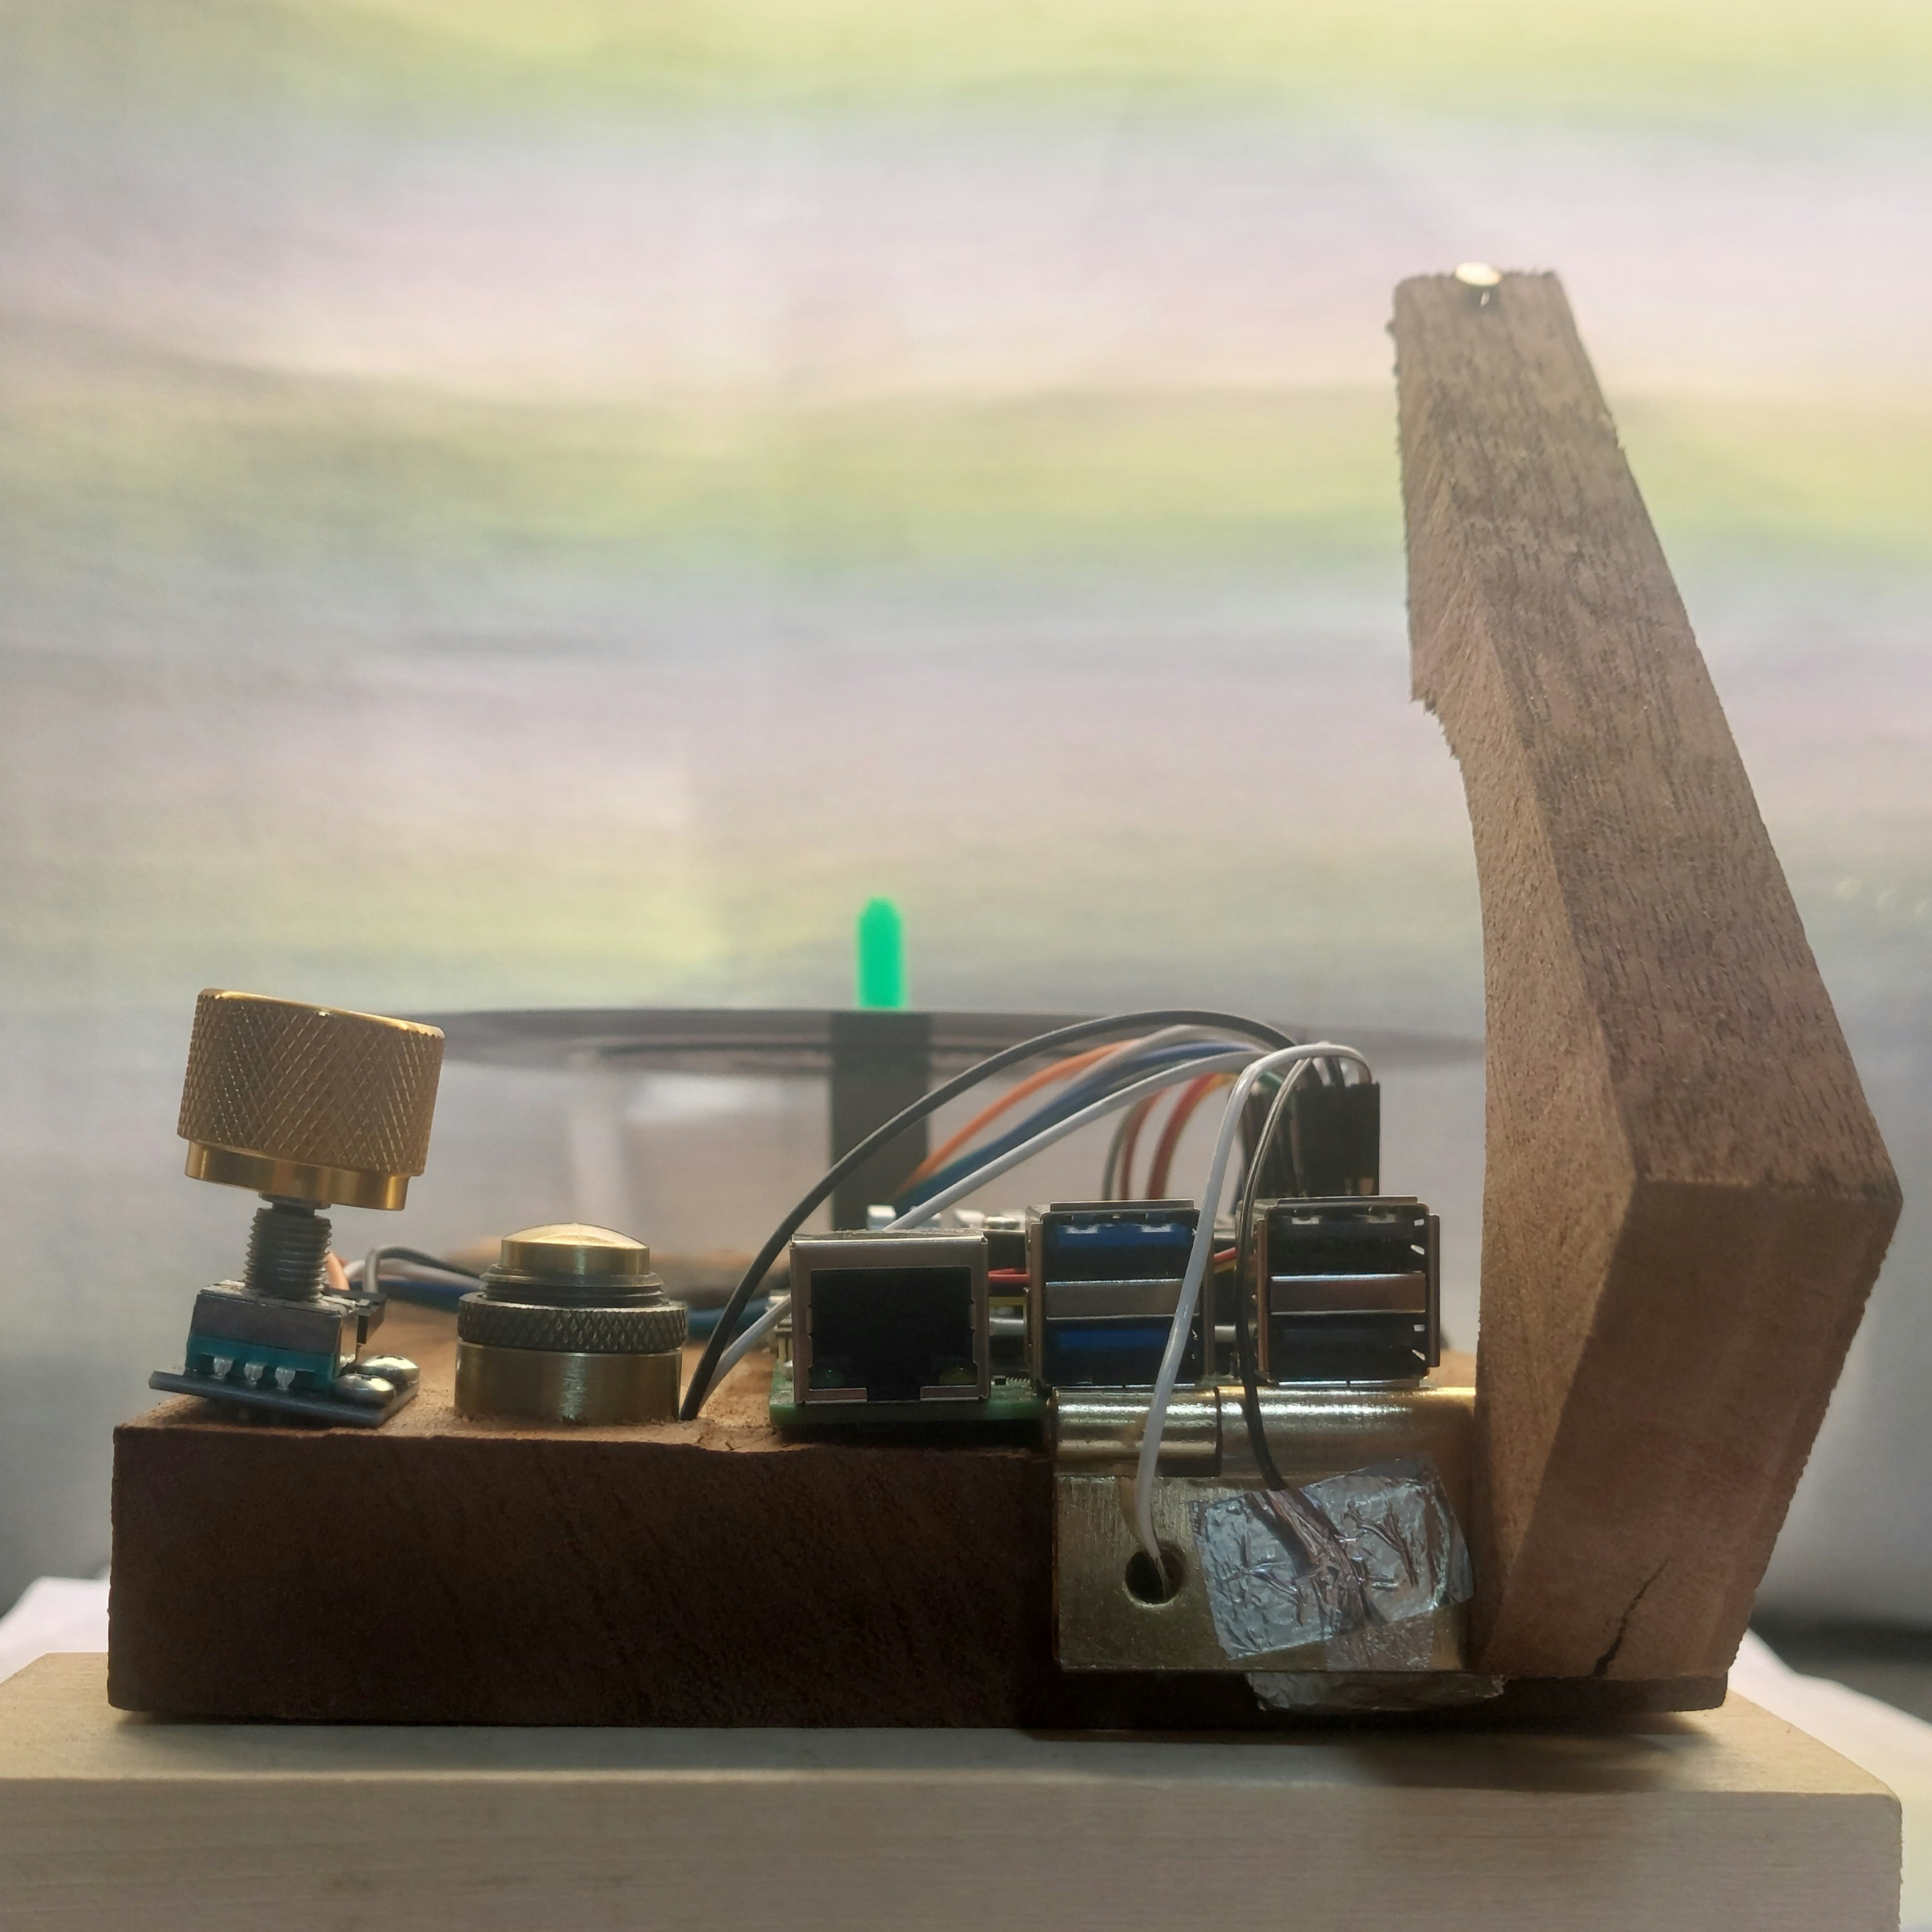
\includegraphics[width=\textwidth]{images/photos/profile_SIDE.jpg}
                    \caption{`Near' side profile of the device}
                    \label{fig:side1}
                \end{minipage}
                \hfill
                \begin{minipage}[b]{0.225\textwidth}
                    \centering
                    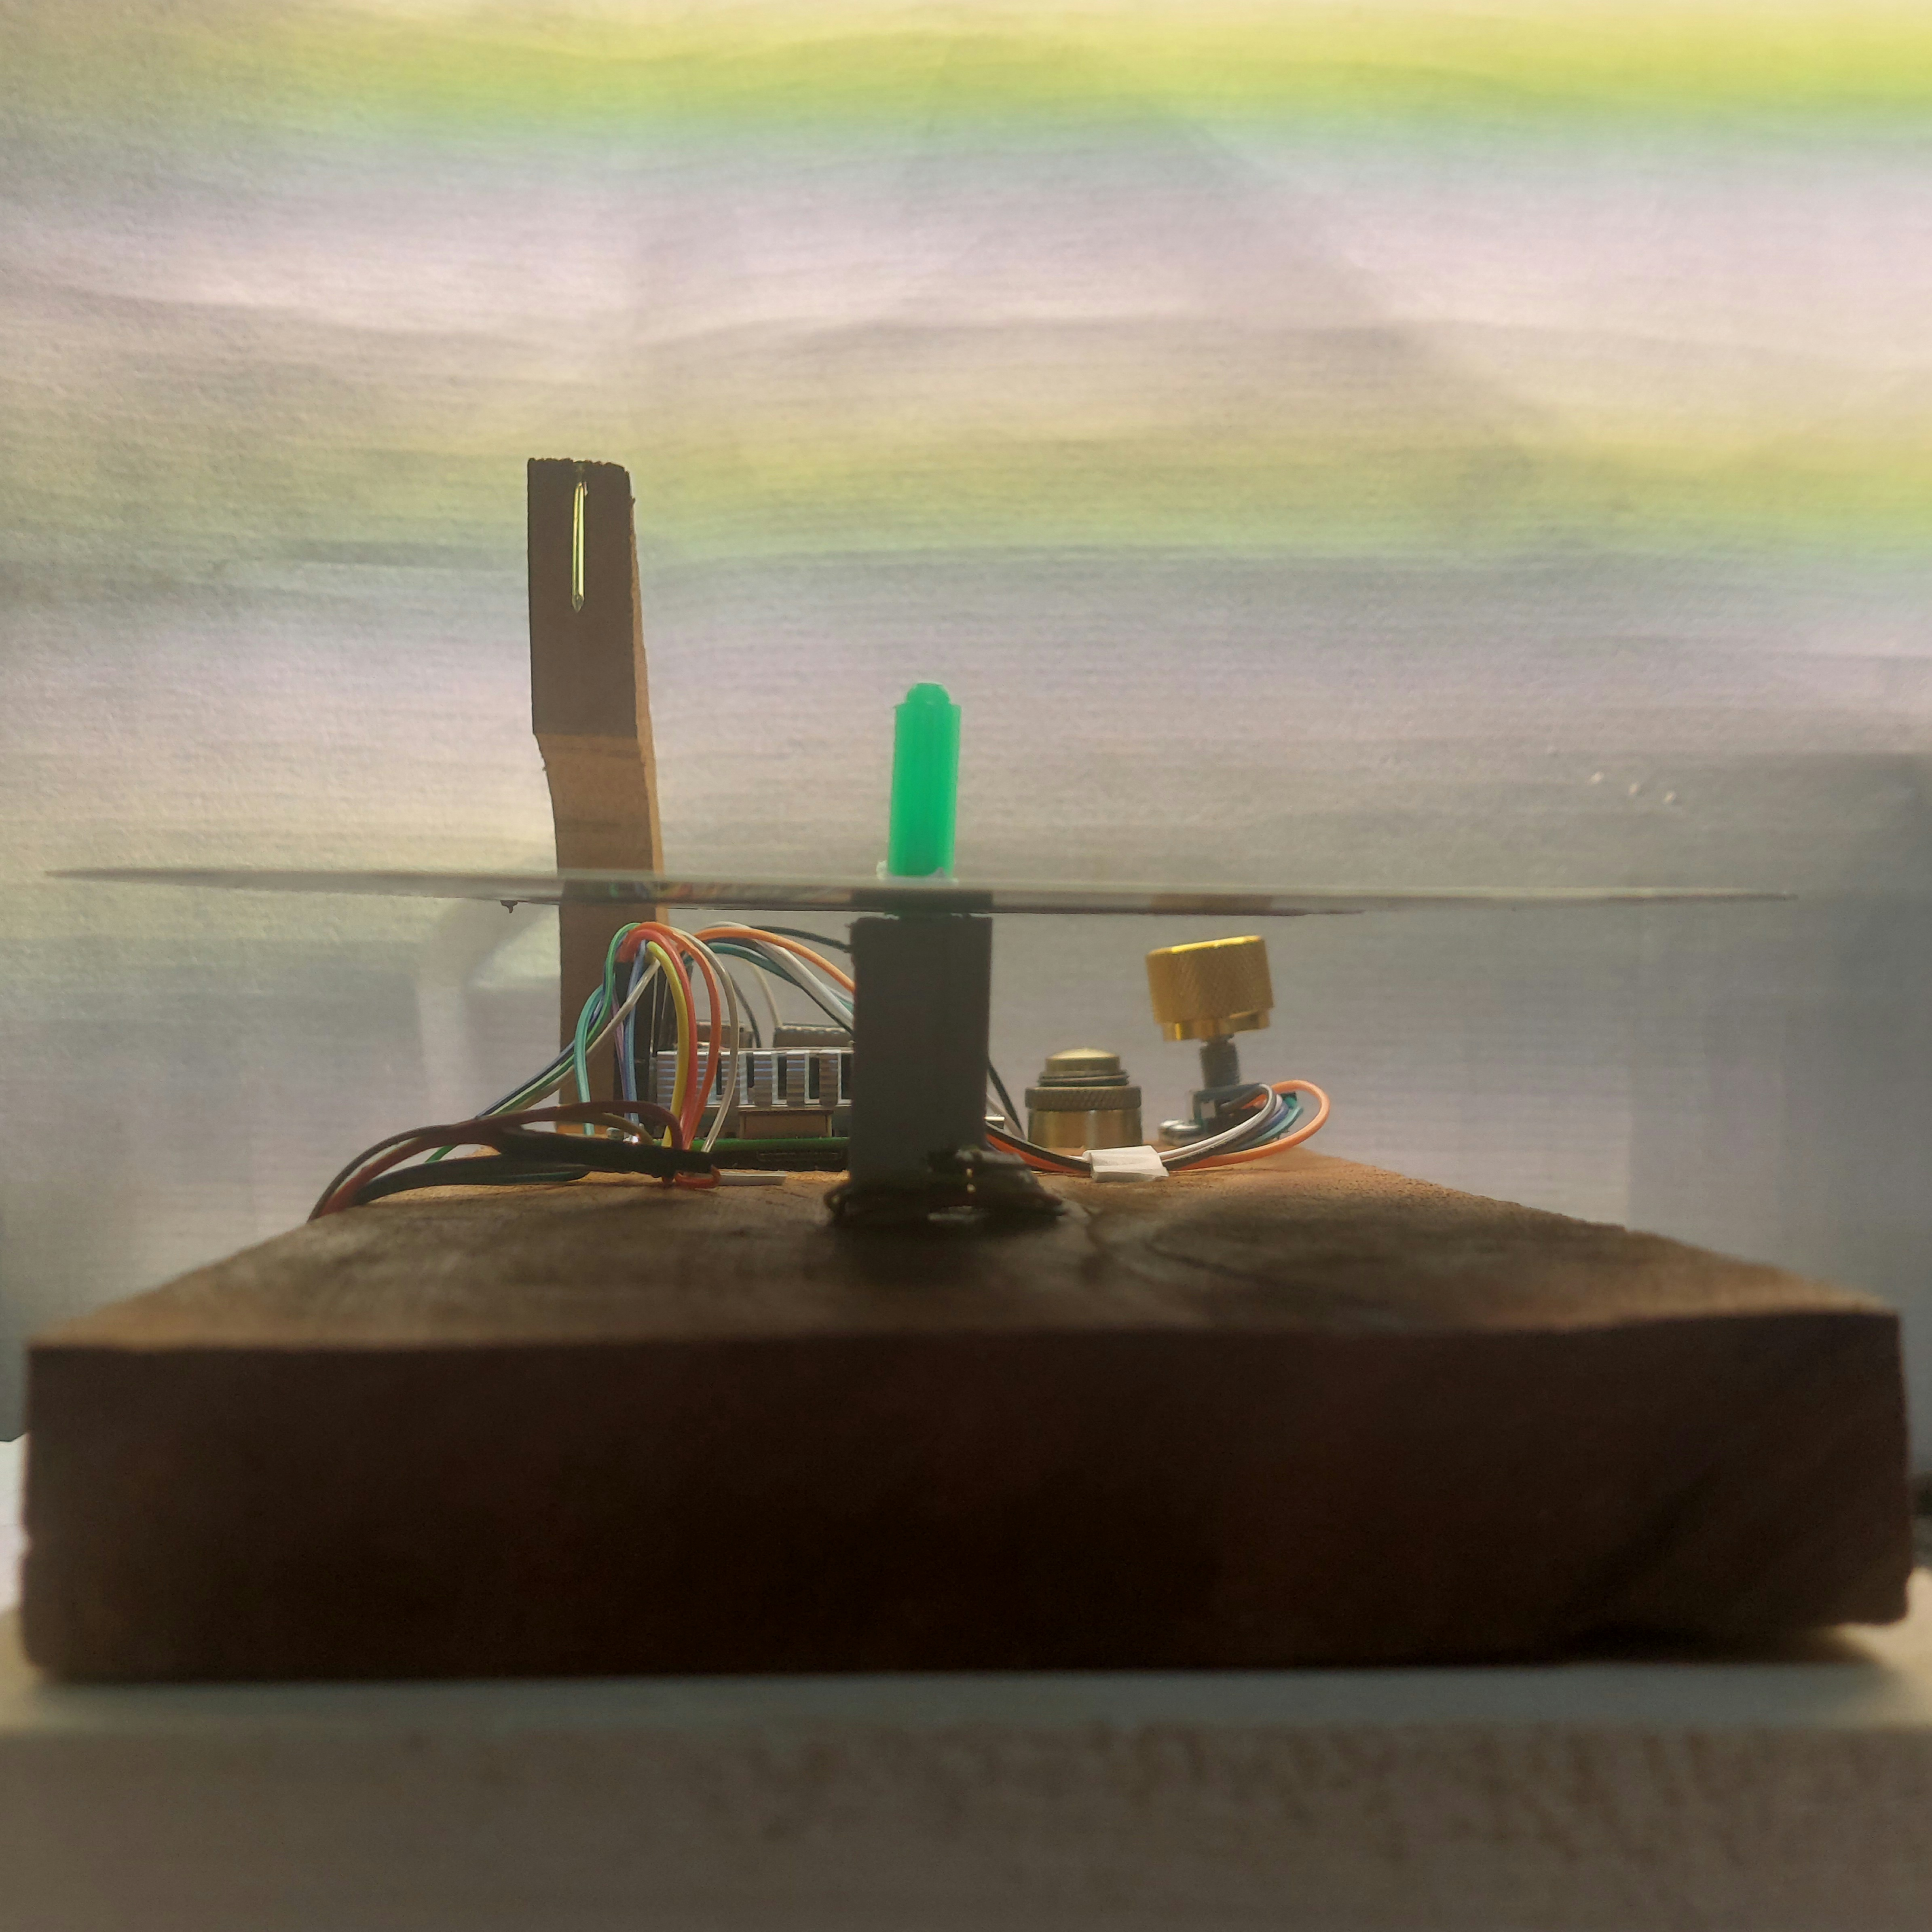
\includegraphics[width=\textwidth]{images/photos/profile_SIDE2.jpg}
                    \caption{`Far' side profile of the device}
                    \label{fig:side2}
                \end{minipage}
                \hfill
                \begin{minipage}[b]{0.45\textwidth}
                    \centering
                    \includegraphics[width=\textwidth]{images/photos/profile-BOTTOM.jpg}
                    \caption{Bottom-up profile of the device}
                    \label{fig:bottom}
                \end{minipage}
            \end{figure}
    
        \subsection{Integrated Hybrid System}
    
            Combining the above, the complete product functions as a fully standalone smart vinyl player. The projection-based host interface is displayed directly onto the disc surface during playback. The interface dynamically updates based on system state (e.g., track change, album detected) and user input.
    
            Figures~\ref{fig:wotw}–\ref{fig:colne} show the system in use, including full interactive mode and the passive, minimal visual state.
    
            \begin{figure}[h]
                \centering
                \begin{minipage}[b]{0.45\textwidth}
                    \centering
                    \includegraphics[width=\textwidth]{images/photos/wotw-ui.jpg}
                \end{minipage}
                \hfill
                \begin{minipage}[b]{0.45\textwidth}
                    \centering
                    \includegraphics[width=\textwidth]{images/photos/wotw.jpg}
                \end{minipage}
                \label{fig:wotw}
                \caption{Front-end UI projected onto device, with interactive interface (left) and minimal interface (right).}
            \end{figure}
            
            \begin{figure}[h]
                \centering
                \begin{minipage}[b]{0.45\textwidth}
                    \centering
                    \includegraphics[width=\textwidth]{images/photos/colne-ui.jpg}
                \end{minipage}
                \hfill
                \begin{minipage}[b]{0.45\textwidth}
                    \centering
                    \includegraphics[width=\textwidth]{images/photos/colne-ui-zoom.jpg}
                \end{minipage}
                \label{fig:colne}
                \caption{Front-end UI projected onto device, with full interactive interface.}
            \end{figure}
    
            % TODO cite videos here, too
    
    %%%%%%%%%%%%%%%%%% SECTION 6 %%%%%%%%%%%%%%%%%%
    \section{Evaluation}
        % does it do what it is supposed to do?
        % how well?
        % how well against others?
    
        This section evaluates the system’s effectiveness in meeting its goals, considering both quantitative performance and qualitative experience. Evaluation is divided into four areas: technical performance, user experience, comparison with existing workflows, and broader implications.
    
        Quantitative metrics include classification accuracy, metadata reliability, system responsiveness, and code robustness. Qualitative factors assess usability, aesthetics, and the hybrid nature of the physical and digital design. Finally, the system is compared against alternative methods, with discussion of limitations, trade-offs, and ethical considerations.
        
        \subsection{Quantitative Evaluation}
    
            \subsubsection{Album Classification Accuracy}
    
                To assess classification accuracy, the model was trained on the full dataset and evaluated on a held-out test set of 34 images. It achieved a top-1 accuracy of 91.18\%, correctly predicting 31 out of 34 albums. Of the three errors, two were due to the model being trained on visually distinct variant covers (see Figure~\ref{fig:ModelEval}), with only one test image matching the training version. If these variant covers are treated as anomalies, the accuracy rises to 97.05\%. While the test set is relatively small and not exhaustive, it reflects a reasonable physical collection a user might own.
    
                \begin{figure}
                    \centering
                    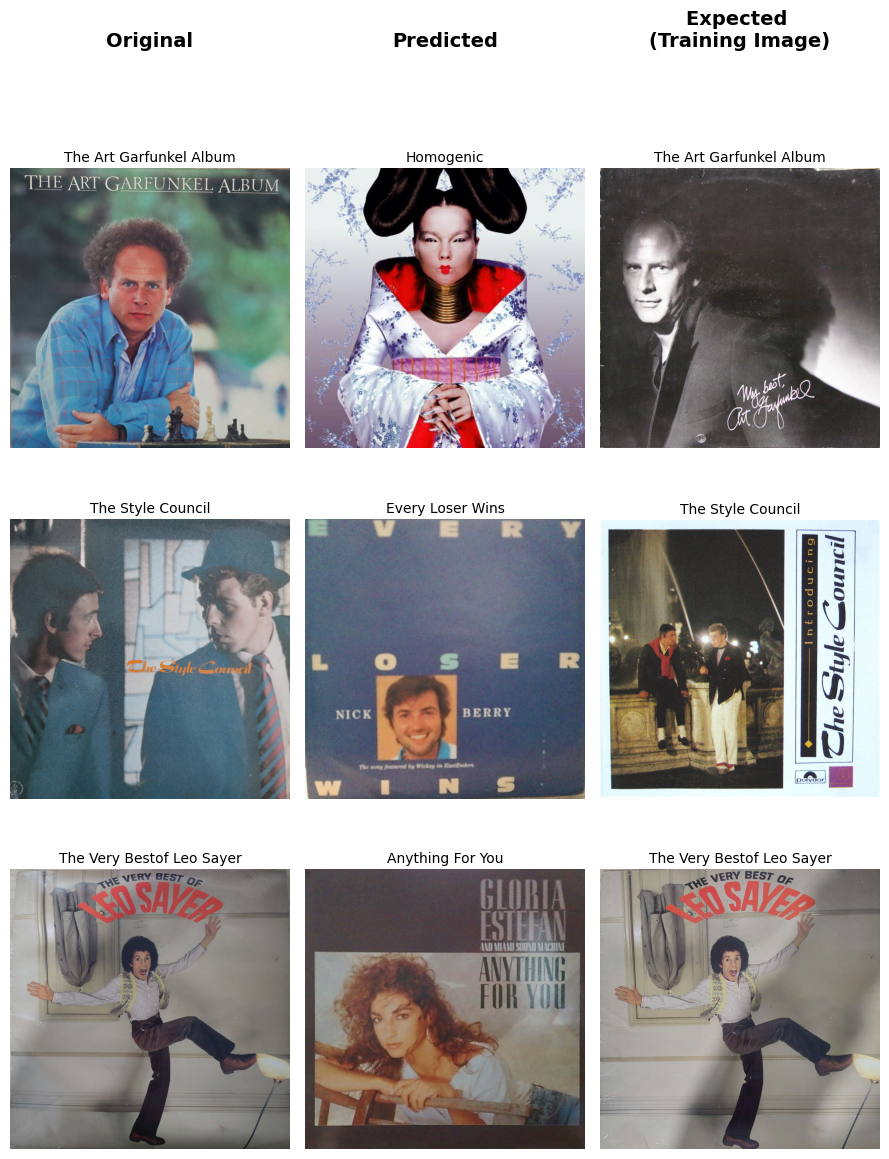
\includegraphics[width=0.5\linewidth]{images/modelEval.png}
                    \caption{Examples of misclassifications from the validation set}
                    \caption*{
                        Each row shows a failure case: the original input image (left), the model’s incorrect prediction (centre), and the correct training image (right). Errors primarily occured due to cover variants.
                    }
                    \caption*{
                        Artworks are © their respective copyright owners.
                    }
                    \label{fig:ModelEval}
                \end{figure}
    
            \subsubsection{Metadata Retrieval Accuracy}
    
                Since metadata retrieval depends on external sources and network responses, evaluation was performed manually. A representative set of 32 albums was tested using automated centre-level retrieval. Of these, 4 were exact matches, 8 were correct but returned variant covers (e.g., CD editions), 2 matched the correct artist but wrong album, 15 returned no label, 2 returned unrelated images, and 1 returned an entirely incorrect label. In addition to the centre label, the Spotify album is also selected, which affects the textual metadata and album cover shown on remote devices. Of these same albums, 3 albums were compilations not present on Spotify, which led to retrievals of other compilations with similar themes (e.g., disco, Bond themes, Christmas). One album was a musical, correctly identified by title but with different performers, and one “best of” album was not available on Spotify, but yielded the correct artist. Despite some gaps, most queries retrieved results that were either correct or thematically relevant. With only a fairly low percentage of fetching bad data from Spotify (84.38\%; up to 96.88\% excluding compilations) the primary metadata source is correct, and as this only failed for particularly niche albums, a more standard collection should be very robust in the system.
    
                The centre label system was less reliable, yielding a relevant result only 43.75\% of the time, with a correct label only 37.5\%; however, as this only serves additional supplementary data, this is an acceptably low success rate. Particularly as a user could add their own image samples to the system's cache directory, fixing this problem. However, future improvements to this pipeline would certainly be beneficial.
    
    
            \subsubsection{System Responsiveness}
    
                Responsiveness was measured by timing the interval between user input (e.g., cover upload or classification trigger) and result delivery. The system was treated as an end-to-end pipeline. Tests across varying devices and network conditions showed average response times of under 2 seconds for classification and under 4 seconds for metadata retrieval, using the Ouroboros model trained on the full dataset. Worst-case latency occurred on slower connections, reaching up to 7 seconds. Overall, the system remained responsive and usable across typical usage scenarios.
    
            \subsubsection{Code Robustness}
    
                The codebase was evaluated through a suite of automated unit tests, covering core components such as image processing, metadata retrieval, and classification logic. The overall test pass rate is reported, and code coverage was estimated to ensure critical paths are exercised. No critical failures or regressions were observed during testing.
    
                The frontend achieved an average of 71.5\% statement coverage, with particularly strong performance in components like WebSocketManager.ts (96\%) and SpotifyPlayer.ts (92.4\%). The backend reached 66.2\% average coverage across core Python modules, with several key files such as sessionManager.py, stateManager.py, and modelHandler.py reaching very high coverages of 89–100\%. However, some components — notably main.py, routes.py, and training utilities — remain untested due to their hardware dependence or being out of scope.
                
                Overall, the combined project-wide coverage stands at 71.5\%, reflecting a strong foundation with room for expanding test coverage to the integration and hardware layers.
    
        \subsection{Qualitative Evaluation}
    
            To evaluate the emotional, aesthetic, and practical experience of the system, a user study was conducted with 17 participants. These users were surveyed after physically using the system, either through direct interaction or a guided session.
    
            Due to the nature of the device -- a physical prototype requiring in-person use—there were significant constraints in recruiting participants. Access to the system was necessarily limited to those who could be reached directly, meaning the sample primarily consisted of friends, family, and peers. Additionally, many users only had brief interaction windows, limiting the depth of familiarity they could develop.
            
            This sample bias is acknowledged. There is likely a positive skew in the responses due to personal connection and the novelty of the system. However, efforts were made to prompt critical feedback, and not all responses were favourable. While this limits generalisability, the feedback gathered still offers valuable insight into the usability, aesthetic reception, and conceptual strengths of the system.
    
            Feedback was collected via a structured Google Form following hands-on use of the system. The form included a combination of scaled questions and optional free-text responses, covering usability, satisfaction, convenience, and scanning accuracy. Responses also captured listening habits and attitudes toward physical media, providing broader context for interpreting user experience.
        
            \subsubsection{User Experience -- Usability}
                User testing focused on how intuitive the system felt to new users. Survey data from 17 participants showed a mostly positive trend:
                
                    76.5\% of users rated ease-of-use at 3 or higher,
                
                    with 35.3\% rating it 5 (very easy).
                    Only one user rated it as very difficult (1), citing a lack of initial instruction.
                
                Notable feedback highlighted the importance of a clear onboarding process, with one user commenting that "the layout was good, but I didn’t know what to do at first." Others praised its familiarity, especially those with vinyl experience, describing the interface as "intuitive and natural."
                
                These results suggest that while the system is broadly accessible, it benefits significantly from prior exposure to analogue devices and would be improved by minimal visual guidance or prompts on first use.
    
            \subsubsection{User Experience -- Aesthetics}
                From the 17 responses, 70.6\% of participants who had experience with vinyl cited aesthetics as a key reason for ownership. This was reflected in comments such as "felt more immersive than expected" and "tactile feedback made it feel authentic."
    
                Design choices such as the use of real turntable elements, album art display, and the physical-digital hybrid interaction were positively received. Users described the system as "satisfying to use" and "visually rich."
                
                These findings indicate strong aesthetic engagement, aligning well with the nostalgic and cultural associations users have with vinyl.
            
        \subsection{Comparative Analysis}
            
            The system sits at the intersection of traditional vinyl playback and modern digital music access. Compared to standard streaming platforms, it introduces a tangible, physical interaction absent from purely digital interfaces. While streaming services offer convenience and breadth of access, they lack the ritual and aesthetic value that this system provides.
    
            In contrast to traditional record players, this system offers automatic metadata enrichment, playback synchronisation via Spotify, and album recognition—features not available in analogue setups. However, it cannot match the audio fidelity or full physicality of actual vinyl playback.
            
            Compared to mobile apps that scan album covers (e.g., Shazam or Discogs), this system is less portable but more immersive. Its strength lies in offering a hybrid experience—inviting physical interaction while integrating smart digital features.
    
            In informal benchmarks, this system’s full album identification-to-playback cycle averaged $\approx 6.2$s. By contrast, Spotify search averages $\approx 3$s (but lacks physical input, and relied on existing user knowledge of the album details), while manual lookup via Discogs took over $\approx 20–30$s. Although slower than pure-digital workflows, the hybrid interaction offers a richer, more deliberate experience.
    
        \subsection{Limitations and Trade-offs}
    
            A key limitation is the need for physical access to the system, which reduces scalability and reach. The classification model, while highly accurate on common albums, is less reliable on niche or variant covers. Metadata retrieval also depends on external APIs, and can occasionally produce incomplete or inaccurate results.
    
            From a technical standpoint, the system balances performance with simplicity, but lacks full robustness in edge cases (e.g., compilation albums or Spotify mismatches). Code coverage is strong but not complete, particularly around hardware-specific modules.
            
            There is also a trade-off between convenience and intentionality: while less convenient than streaming, the system offers a more deliberate and engaging listening experience -- by design.
    
        \subsection{Ethical Implications}
            
            This project prioritised ethical considerations throughout its lifecycle. Unlike generative AI systems, which often replicate or compete with original works, this classifier respects artistic integrity by not creating derivative content, nor redistributing copyrighted material.
            
            The system was designed to promote rather than replace physical media, aligning with the commercial interests of creators. Classification results are used solely to redirect users to legitimate playback platforms, potentially supporting royalties. No training data is exposed or accessible to users, and all datasets were acquired only from services explicitly permitting such use.
            
            Accessibility and openness were central goals -- with digital parity ensuring inclusive interaction, and full source availability supporting transparency and academic reuse. The project maintains a clear distinction between legal compliance and ethical responsibility, aiming to exceed beyond minimum standards in both.
    
    %%%%%%%%%%%%%%%%%% SECTION 7 %%%%%%%%%%%%%%%%%%
    \section{Conclusions and future work} % edit section heading as appropriate
        \subsection{Conclusions}
        % summarise results
    
            This project successfully met its core aims: building a fully functional hybrid media system that integrates physical interaction with digital music streaming (as shown in Tables~\ref{tab:FR}-\ref{tab:NFR}). Quantitative results showed strong model performance (91.18\% top-1 accuracy), fast response times (under 4s average), and solid code robustness (71.5\% coverage). Qualitative testing confirmed that users found the system intuitive and aesthetically engaging, with particular praise for its nostalgic design and physical-digital interaction.
    
            Limitations such as metadata inconsistency and edge-case classification were identified and mitigated where possible. User feedback revealed opportunities for clearer onboarding, but overall usability was high. Comparisons against existing tools underscored the novelty and experiential value of the system.
    
            \begingroup
                \renewcommand\thefootnote{}\footnotetext{Some deeper, yet more tangential thoughts are given in Appendix~\ref{sec:nailArt}, reflecting on the symbolic and aesthetic aspects of the system, beyond the scope of formal evaluation.}
                \addtocounter{footnote}{-1}
            \endgroup
    
        % achieved aims?
        \begin{longtable}{|c|p{5cm}|c|p{5cm}|}
            \caption{Evaluation of Functional Requirements} \label{tab:FR}\\
            \hline
            \textbf{ID} & \textbf{Requirement} & \textbf{Met?} & \textbf{Comment} \\
            \hline
            \endfirsthead
            \hline
            \textbf{ID} & \textbf{Requirement} & \textbf{Met?} & \textbf{Comment} \\
            \hline
            \endhead
            FR1 & Image recognition accuracy ≥90\% & Yes & Achieved 91.18\% top-1 accuracy (97.05\% if cover variants excluded). \\
            \hline
            FR2 & Playback initiation within 5 seconds & Yes & Average response time under 4 seconds; peak latency 7s on poor networks (initial assumptions included good connection). \\
            \hline
            FR3 & Integration with Spotify API & Yes & Functional integration achieved; metadata retrieved for 84.38\% of albums. \\
            \hline
            FR4 & Software playback controls & Yes & Users could reliably play/pause/skip tracks via the interface. \\
            \hline
            FR5 & Clear track/album information display & Yes & Displayed metadata from Spotify when available. \\
            \hline
            FR6 & Intuitive UI suitable for non-technical users & Yes & 76.5\% of users found it easy to use; onboarding could improve. \\
            \hline
            FR7 & Physical playback controls & Yes & Tactile controls implemented; users responded positively to physicality. \\
            \hline
        \end{longtable}
    
        \begin{longtable}{|c|p{5cm}|c|p{5cm}|}
            \caption{Evaluation of Non-Functional Requirements} \label{tab:NFR}\\
            \hline
            \textbf{ID} & \textbf{Requirement} & \textbf{Met?} & \textbf{Comment} \\
            \hline
            \endfirsthead
            \hline
            \textbf{ID} & \textbf{Requirement} & \textbf{Met?} & \textbf{Comment} \\
            \hline
            \endhead
            NFR1 & System latency ≤5 seconds & Yes & All processing within 4s on average; met under typical use. \\
            \hline
            NFR2 & System uptime ≥99\% & Yes & No runtime crashes observed in testing; highly stable during sessions. \\
            \hline
            NFR3 & Graceful handling of recognition failures & Partial & Errors redirected cleanly with fallback behaviour or retry prompts. Greater specificity in error messages could be improved. \\
            \hline
            NFR4 & Compatibility with Raspberry Pi 5 & Yes & Fully developed and deployed on Raspberry Pi 5 hardware. \\
            \hline
            NFR5 & Clear documentation for easy setup & Yes & Instructions and bash scripts provided. \\
            \hline
            NFR6 & Compliance with UK copyright laws & Yes & Use justified under CDPA fair dealing; no distribution of copyrighted media, beyond educational scope of report contents. \\
            \hline
            NFR7 (1) & Compliance with Spotify API Terms & Yes & Spotify data only used for playback; model training did not breach API terms. \\
            \hline
            NFR7 (2) & Compliance with Discogs API Terms & Yes & Discogs data only used for playback; model training did not breach API terms. \\
            \hline
            NFR7 (3) & Compliance with Cover Art Archive API Terms & Yes & TODO. \\
            \hline
        \end{longtable}
    
        % improvements!
        
        \subsection{Future work}
          % ideas for further work
          % big ideas; what could be done with my project?
          Several directions exist for extending this project:
    
          \paragraph{Improving album detection with retraining and real-time augmentation}
    
          Whilst the Hydra expandable PNN model experiments were promising, they did not manage to mature into a usable production-grade state within the project's timespan. Future work into this model could be done to allow the system to be truly robust by allowing users to seamlessly add new albums to their collection, without losing performance quality.
    
          This could be taken even further, by enabling the system to learn from specific corrections made by users, improving classification over time, by regularly re-training the models with reinforcement learning-based `encouragement' and `punishment' weights, using this user feedback.
    
          \paragraph{Onboarding and accessibility}
    
          Add minimal visual prompts, voice guidance, or mobile setup flows to improve ease-of-use for new users.
    
          \paragraph{Expanded integrations}
    
          Extend metadata sources to include lyrics, artist bios, or event listings, or connect fully to other streaming platforms, with the option to seamlessly switch between them on-the-fly (the current system requires manual re-configuration and rebooting of the server).
    
          \paragraph{Deeper HCI research}
    
           Conduct longer-term user studies focused on behaviour, nostalgia, and emotional connection to hybrid interfaces.
    
    %TC:ignore
    %%%%%%%%%%%%%%%%%% REFERENCES %%%%%%%%%%%%%%%%%%
    %\clearpage % uncomment to start on a new page if wanted
    \printbibliography[title={References},heading=bibintoc] % a single list of references for the whole thesis
    
    
    
    %%%%%%%%%%%%%%%%%% APPENDICES %%%%%%%%%%%%%%%%%%
    \begin{uomappendix} 
        % screen dumps of UI
        % important but large results
        \section{Project outline}
    
            \begin{temp}
                Project outline is a required appendix. Put here.
            \end{temp}
            
            % Vinyl is back! According to the \href{https://www.nme.com/news/music/uk-vinyl-sales-2023-reach-highest-level-since-1990-3563676}{NME}, UK sales of vinyl in 2023 were the highest seen since 1990. Vinyl has always remained popular among niche genres, but we are also seeing mainstream artists like Taylor Swift and Lana Del Rey releasing and selling large volumes of albums on the format. Vinyl records have also recently been added into the ONS "Basket of Goods and Services": a carefully selected set of items representative of the goods and services that UK consumers typically spend their money on (\href{https://www.ons.gov.uk/news/news/arecordrevivalthatscookingupastormvinylmusicandairfryersspintheirwayintothebasketofgoods}{ONS}).
            
            % Fans of the format claim better sound reproduction, with a fuller frequency range and a "warmth" lacking in digital formats such as CD. Playing vinyl requires specialist equipment: while the ritual of putting a disc on the turntable and dropping the needle is, for some, part of the experience, it can also be seen as an inconvenience.
            
            % The aim of this project will be to develop an application that supports a blending of the physical and digital worlds. A physical artefact such as an LP is scanned using a camera. The information on the label or cover is then used to identify the release which can be played. This content could be retrieved from a streaming service such as Spotify or Apple Music, an artist site such as \href{https://bandcamp.com/}{Bandcamp}, or the user's own personal media library. This would then allow a user to "play" their records without a turntable. Although the audio quality may not match that of vinyl, such an application would appeal to those who like to collect vinyl for its own sake, or who appreciate the larger format artwork that comes with an old school LP. The application could run on a mobile phone or specialist hardware such as a Raspberry Pi equipped with a camera.
            
            % Example methods that could be used for identification of the release include barcodes, QR codes or OCR acting on label text.
            
            % For a stretch goal, the application could be extended to cover other media: the cassette tape (\href{https://www.theguardian.com/music/2023/apr/20/fun-way-consume-music-why-sales-of-cassette-tapes-soaring}{Guardian}) is also experiencing a comeback, although the \href{https://en.wikipedia.org/wiki/8-track_cartridge}{eight-track} is unlikely to be retrieved from the dustbin of history.
            
            % The project should be considered as challenging. It will require integration of several technologies and some creativity.
        
        \section{Risk assessment}
            \begin{temp}
                Risk assessment is a required appendix. Put here.
            \end{temp}
    
        \section{Model Cards}
            \begin{temp}
                TODO
            \end{temp}
    
        \section{Datasets}
    
            \subsection{Training Set 'Mini'} \label{data:mini}
    
                15 albums; 24 data points
    
            \subsection{Training Set 'Large'} \label{data:large}
    
                \ref{data:mini}
                
                + 68 classes; + 133 data points (a_dig)
    
                + 20 classes; + 39 data points (b_phys)
    
            \subsection{Training Set Augmented} \label{data:aug}
    
                \ref{data:large} * 6
    
            \subsection{Validation Set} \label{data:val}
    
                14 albums; 16 data points
    
            \subsection{Test Set} \label{data:test}
    
                \ref{data:val} + 1 class (\_null); + 20 data points
    
        \section{Evaluation Results}
    
            \subsection{Unit Tests}
                \paragraph{Front End}
                \begin{table}[H]
                    \centering
                    \caption{Front-end unit test coverage output (Vitest)}
                    \begin{verbatim}
    -----------------------|---------|----------|---------|---------|
    File                   | % Stmts | % Branch | % Funcs | % Lines |
    -----------------------|---------|----------|---------|---------|
    All files              |    71.5 |    81.81 |   58.71 |    71.5 |
     src                   |   76.76 |    82.08 |   47.27 |   76.76 |
      App.tsx              |   58.64 |    90.24 |   33.33 |   58.64 |
      RemoteController.tsx |   77.91 |    82.85 |      30 |   77.91 |
      VirtualTurntable.tsx |   84.65 |     75.9 |   40.74 |   84.65 |
      WebSocketManager.ts  |      96 |      100 |    90.9 |      96 |
      root.tsx             |       0 |        0 |       0 |       0 |
     src/APIs              |    42.1 |      100 |      60 |    42.1 |
      IMusicAPI.ts         |       0 |        0 |       0 |       0 |
      IMusicPlayer.ts      |    42.1 |      100 |      50 |    42.1 |
     src/APIs/Local        |       3 |        0 |       0 |       3 |
      LocalPlayer.ts       |       3 |        0 |       0 |       3 |
     src/APIs/Spotify      |   76.47 |    94.11 |   72.72 |   76.47 |
      SpotifyAPI.ts        |    66.4 |    92.85 |   66.66 |    66.4 |
      SpotifyPlayer.ts     |    92.4 |       95 |   76.92 |    92.4 |
     src/common            |   72.05 |    66.66 |   70.83 |   72.05 |
      Dialogue.tsx         |    56.6 |     62.5 |   66.66 |    56.6 |
      Tooltip.tsx          |   79.25 |    46.15 |    62.5 |   79.25 |
      WebcamCapture.tsx    |   78.78 |    86.66 |      80 |   78.78 |
     src/types             |     100 |      100 |     100 |     100 |
      Music.ts             |       0 |        0 |       0 |       0 |
      vendor.ts            |     100 |      100 |     100 |     100 |
     src/utils             |     100 |      100 |     100 |     100 |
      blob.ts              |     100 |      100 |     100 |     100 |
    -----------------------|---------|----------|---------|---------|
                    \end{verbatim}
                \end{table}
    
                \paragraph{Back End}
                \begin{table}
                    \centering
                    \caption{Back-end unit test coverage output (Pytest)}
                    \begin{verbatim}
    Name                                          Stmts   Miss  Cover
    -----------------------------------------------------------------
    app\APIs\DiscogsAPI.py                           49      2    96%
    app\APIs\MusicAPI\IMusicAPI.py                   47     13    72%
    app\APIs\MusicAPI\SpotifyAPI.py                 132     61    54%
    app\enums\StateKeys.py                           16      0   100%
    app\main.py                                     182    182     0%
    app\modules\Hardware\IHardwareController.py      31      9    71%
    app\modules\Hardware\piController.py            149    130    13% 
    app\modules\centreLabelHandler.py                70     11    84% 
    app\modules\modelHandler.py                      70      7    90%
    app\modules\sessionManager.py                    48      0   100%
    app\modules\stateManager.py                      35      4    89%
    app\modules\websocketHandler.py                  55     43    22%
    app\routes.py                                   161    161     0%
    app\utils.py                                     35      8    77%
    modelling\__init__.py                             0      0   100%
    modelling\getAlbumArt.py                        131    131     0%
    modelling\models\Amphisbaena.py                 127    109    14%
    modelling\models\BabyOuroboros.py                22     14    36%
    modelling\models\Ouroboros.py                   107     89    17%
    modelling\models\__init__.py                      0      0   100%
    modelling\models\train.py                        87     87     0%
    modelling\models\utils\CustomDataset.py         100     80    20%
    modelling\models\utils\ModelType.py               5      0   100%
    modelling\models\utils\RandomFlip.py             12      4    67%
    modelling\models\utils\Transforms.py              4      0   100%
    modelling\models\utils\__init__.py                0      0   100%
    -----------------------------------------------------------------
                    \end{verbatim}
                \end{table}
    
            \subsection{System Evaluation}
                % \paragraph{Ouroboros Model} \\
    
                \begin{adjustbox}{max width=\textwidth}
                    \begin{lstlisting}[caption={Ouroboros model evaluation results on 34 images}, label={lst:ourobEval}]
    Evaluation Results:
    Total images evaluated: 34
    Correct predictions: 31
    Accuracy: 91.18%
    
    Failures:
    TheArtGarfunkelAlbum_ArtGarfunkel_1984 (Homogenic_Björk_1997)
    TheStyleCouncil_TheStyleCouncil_1983 (EveryLoserWins_NickBerry_1986)
    TheVeryBestofLeoSayer_LeoSayer_1979 (AnythingForYou_GloriaEstefanandMiamiSoundMachine_1988)
                    \end{lstlisting}
                \end{adjustbox}
    
        \section{Image Overflow}
    
            \begin{figure}[H]
                \centering
                \begin{minipage}[b]{0.45\textwidth}
                    \centering
                    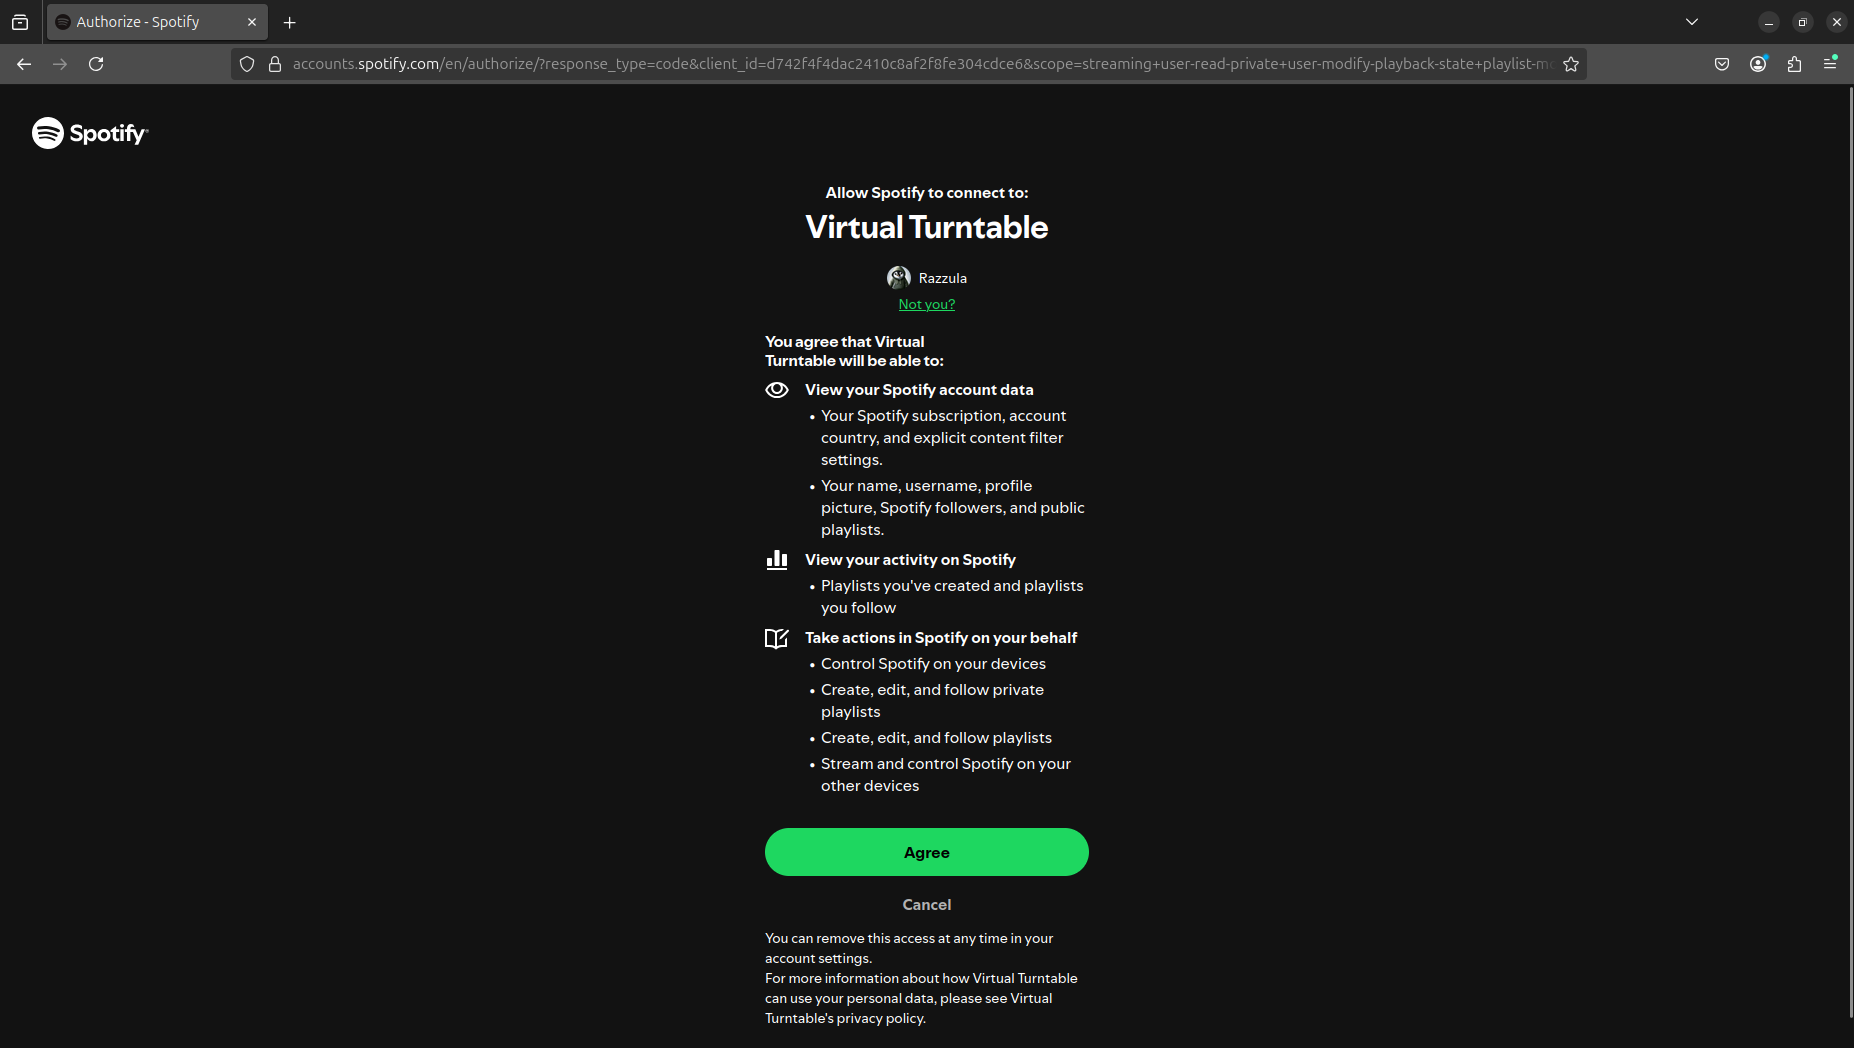
\includegraphics[width=\textwidth]{images/screenshots/HOST_Auth.png}
                    \caption{Screenshot of host client using Spotify's authentication redirection flow}
                    \label{fig:hostAuth}
                \end{minipage}
                \hfill
                \begin{minipage}[b]{0.45\textwidth}
                    \centering
                    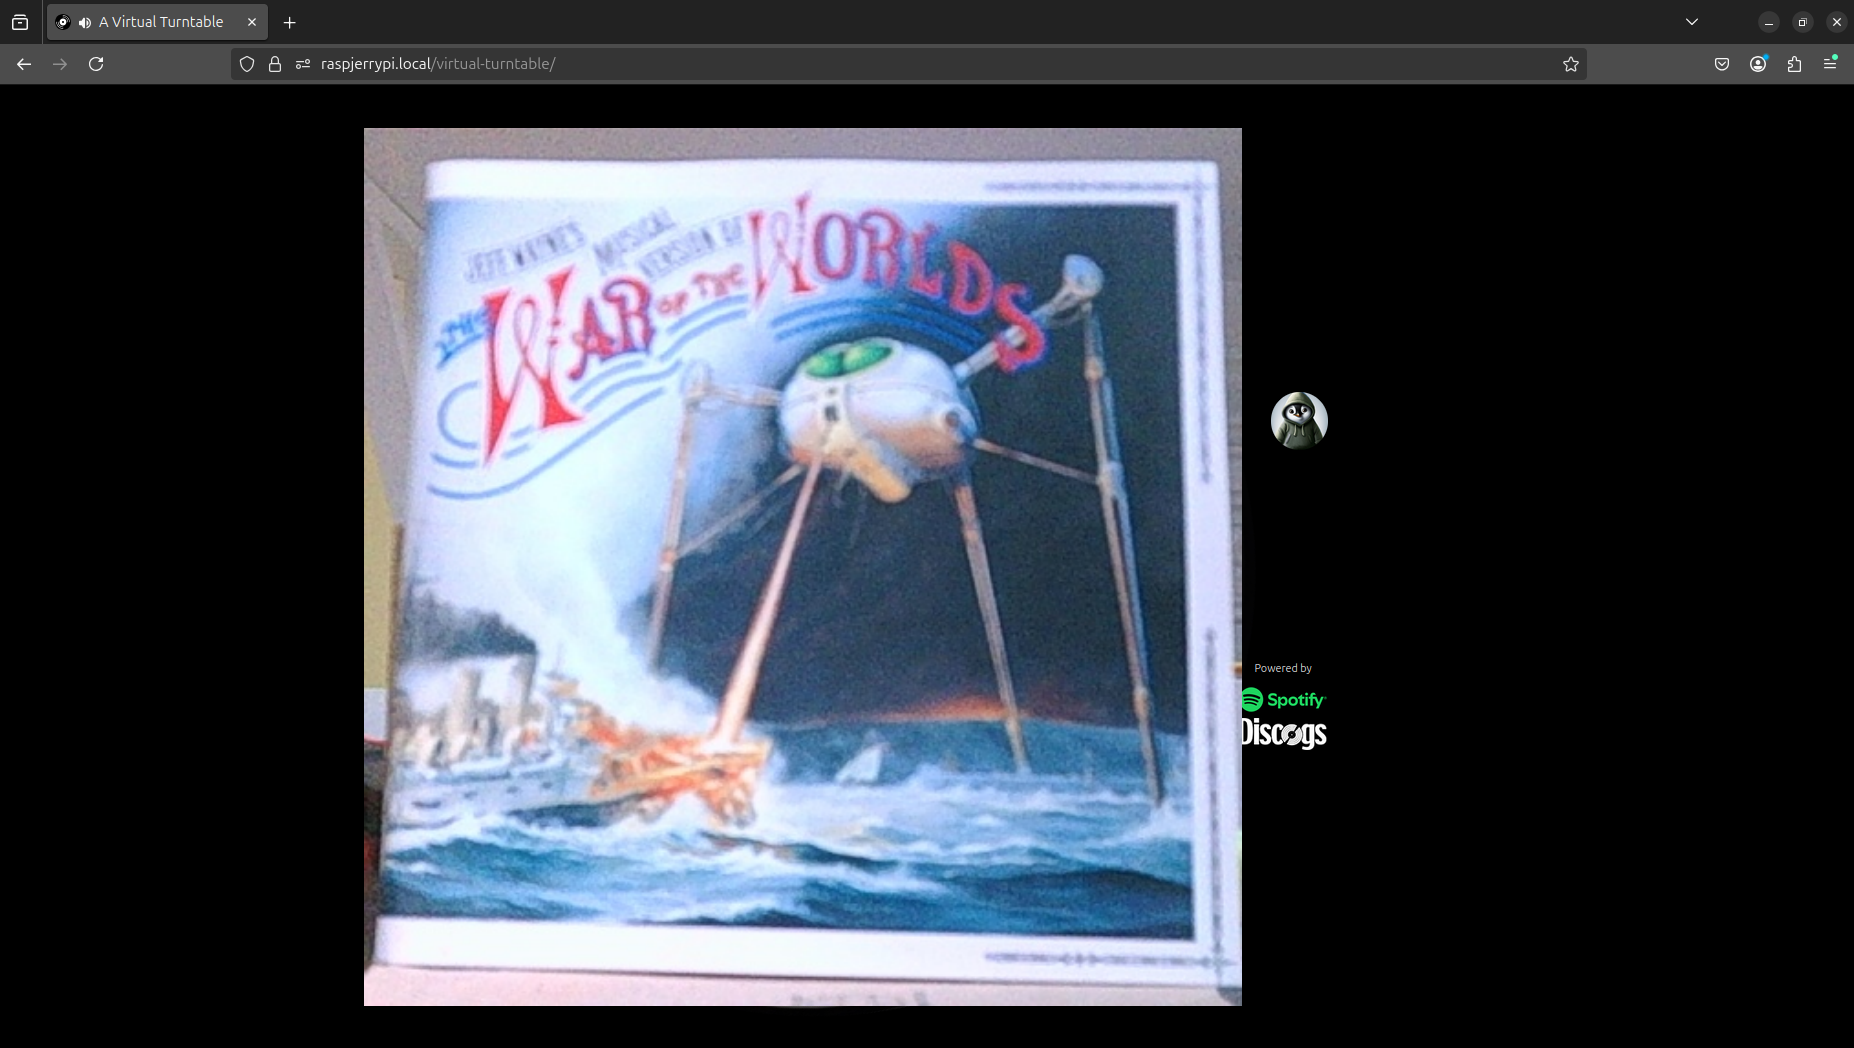
\includegraphics[width=\textwidth]{images/screenshots/HOST_Cam.png}
                    \caption{Screenshot of host client displaying the input image from the camera}
                    \label{fig:hostCam}
                \end{minipage}
                
                \vspace{0.5cm}
                
                \begin{minipage}[b]{0.45\textwidth}
                    \centering
                    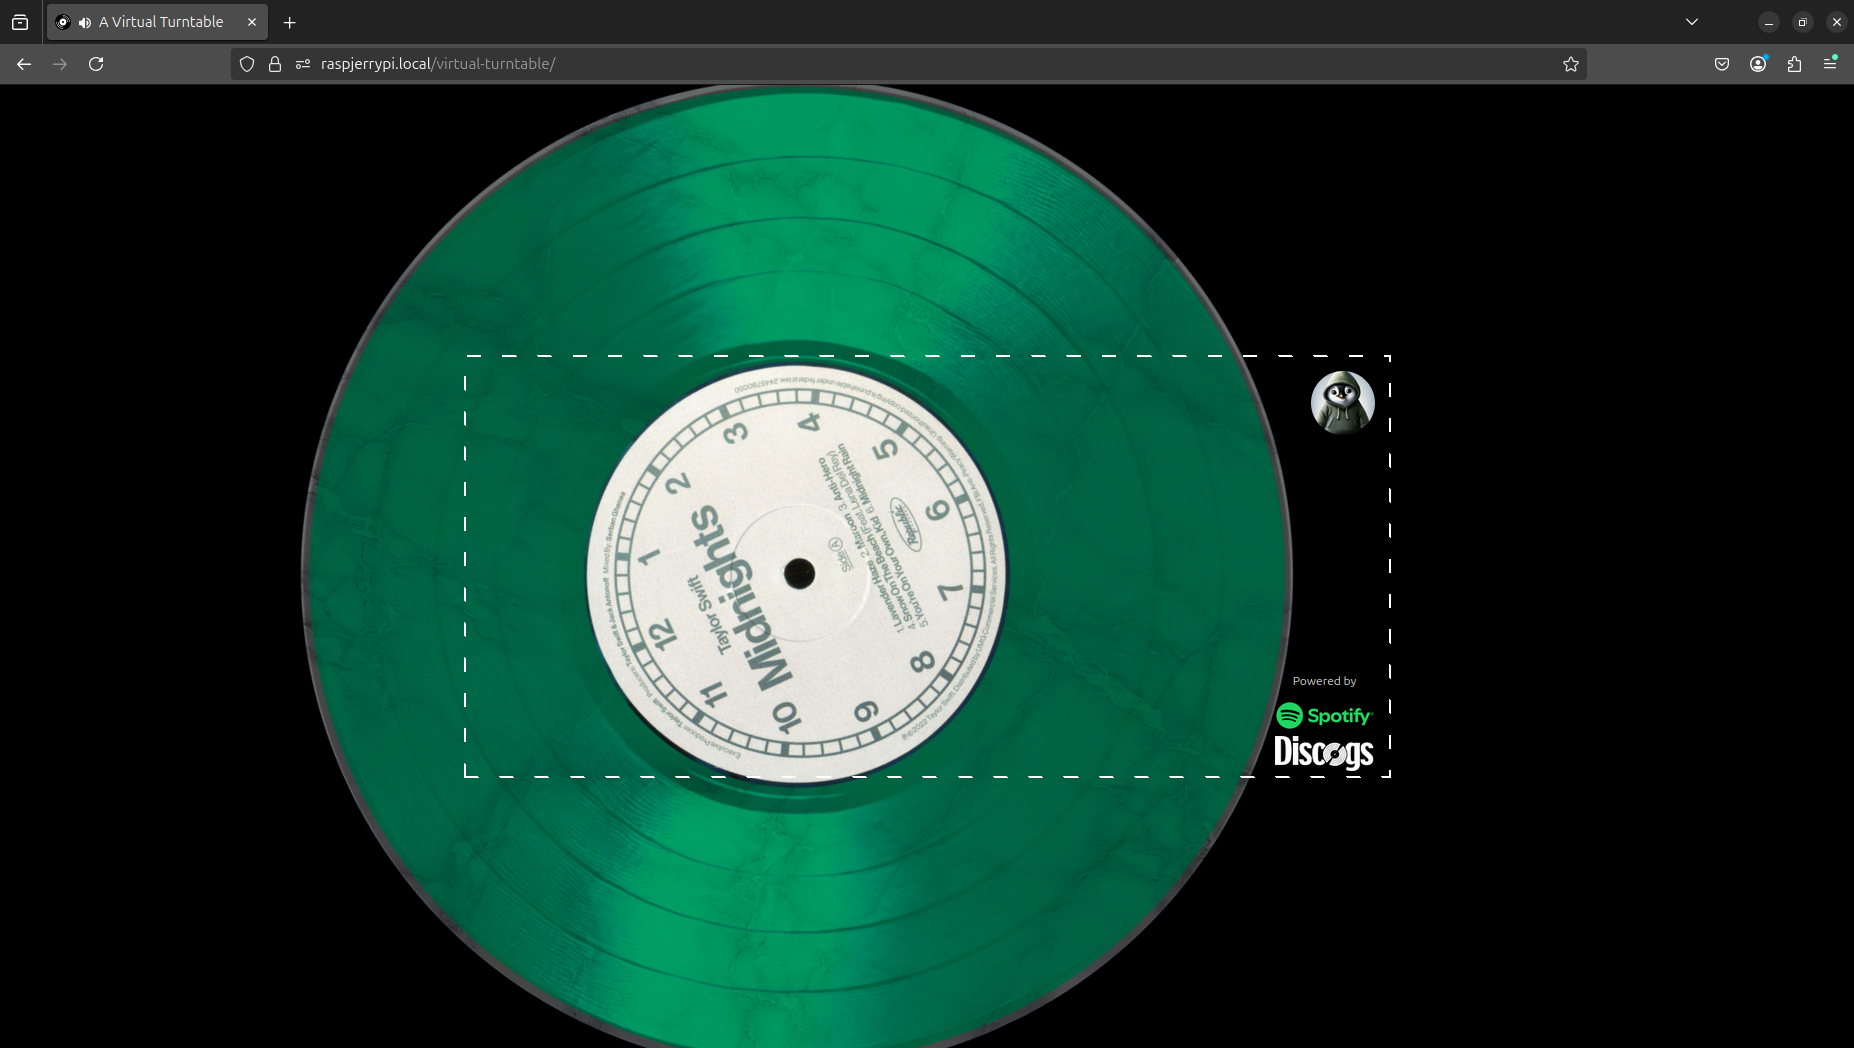
\includegraphics[width=\textwidth]{images/screenshots/HOST_Green.png}
                    \caption{Screenshot of host client using adaptive colouring and texturing}
                    \label{fig:hostGreen}
                \end{minipage}
                \hfill
                \begin{minipage}[b]{0.45\textwidth}
                    \centering
                    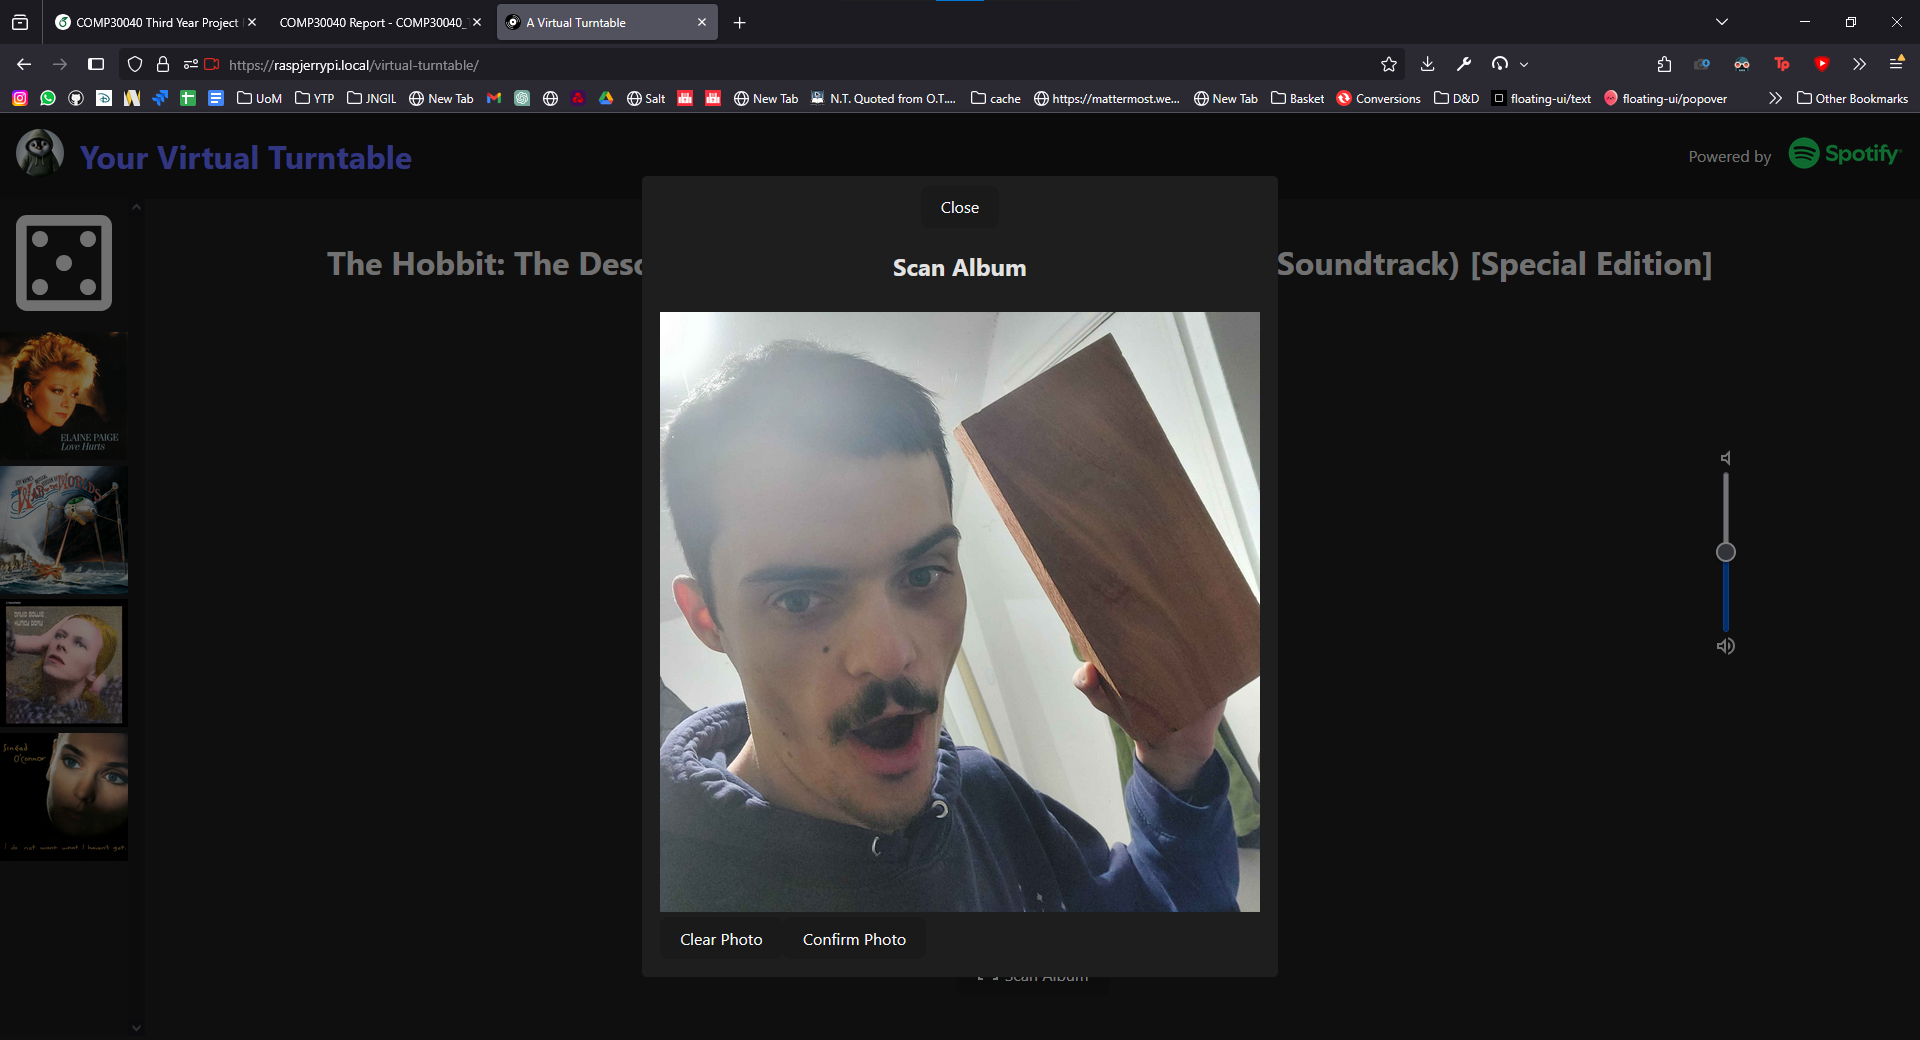
\includegraphics[width=\textwidth]{images/screenshots/LAPTOP_Cam.png}
                    \caption{Screenshot of a remote client (PC) using the camera functionality}
                    \label{fig:laptopCam}
                \end{minipage}
                
                \vspace{0.5cm}
                
                \begin{minipage}[b]{0.45\textwidth}
                    \centering
                    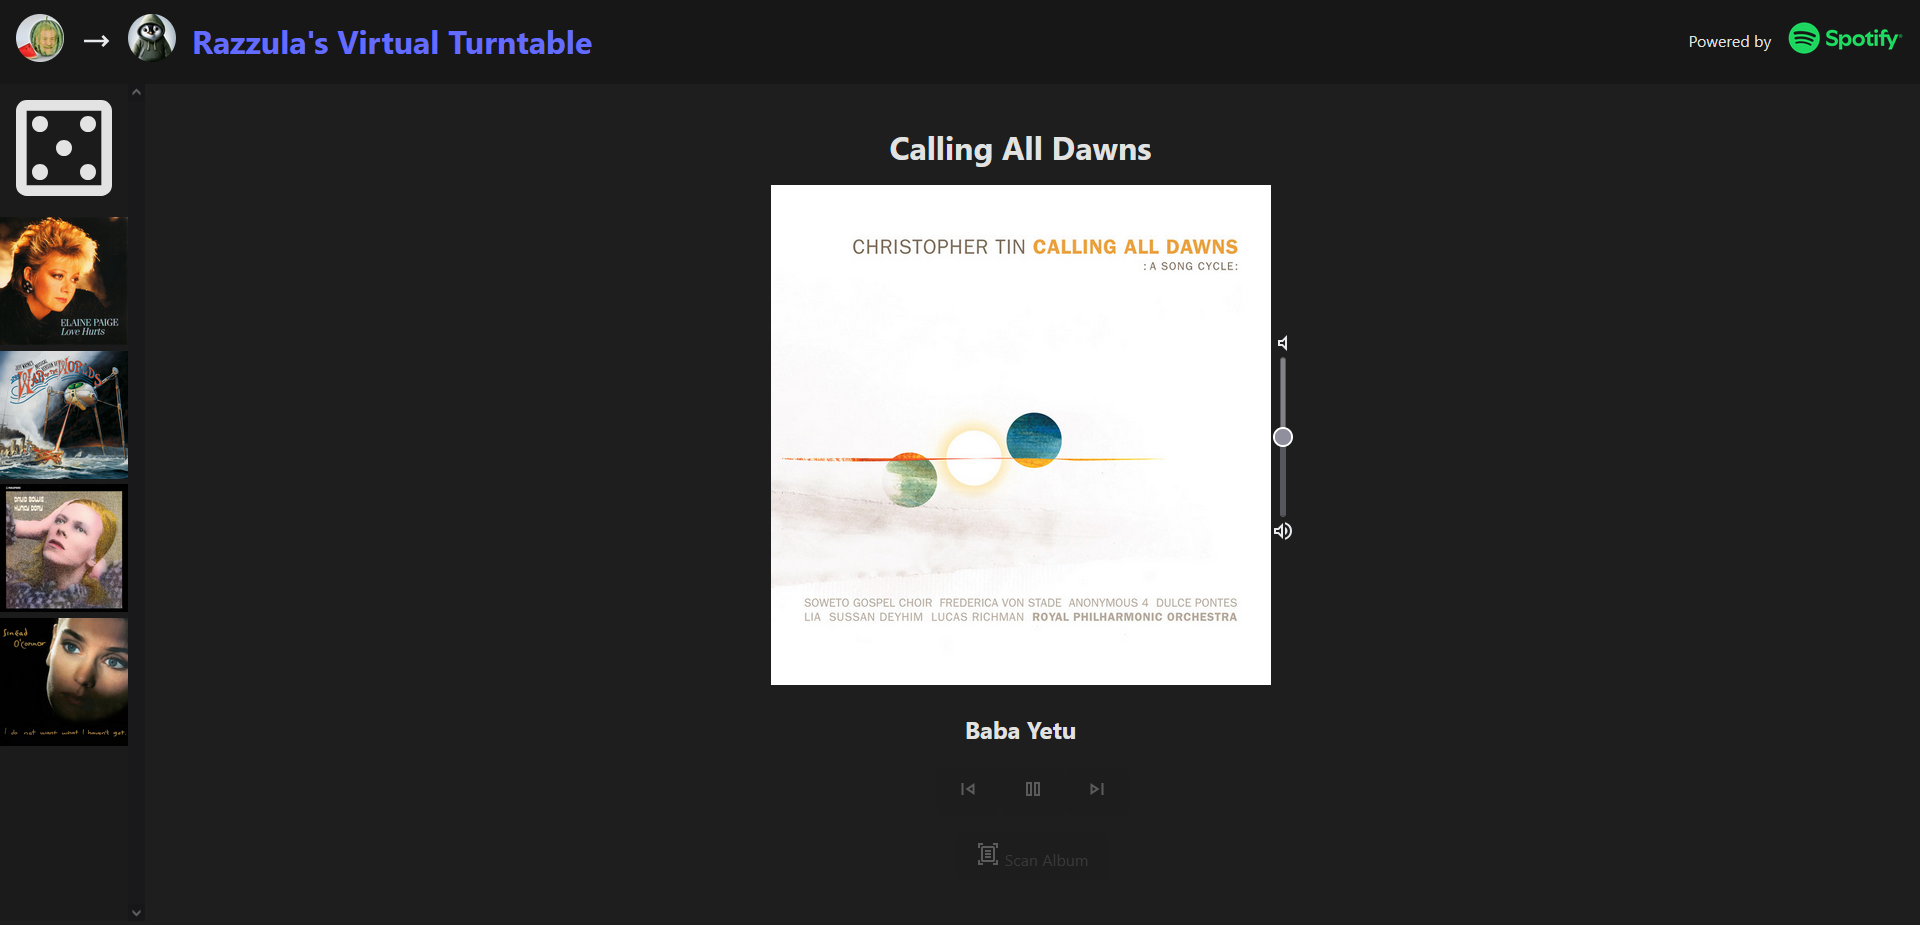
\includegraphics[width=\textwidth]{images/screenshots/LAPTOP_External.png}
                    \caption{Screenshot of a remote client, using an external account (not the host)}
                    \label{fig:laptopExternal}
                \end{minipage}
            \end{figure}
            
            \begin{figure}[H]
                \centering
                \begin{minipage}[b]{0.45\textwidth}
                    \centering
                    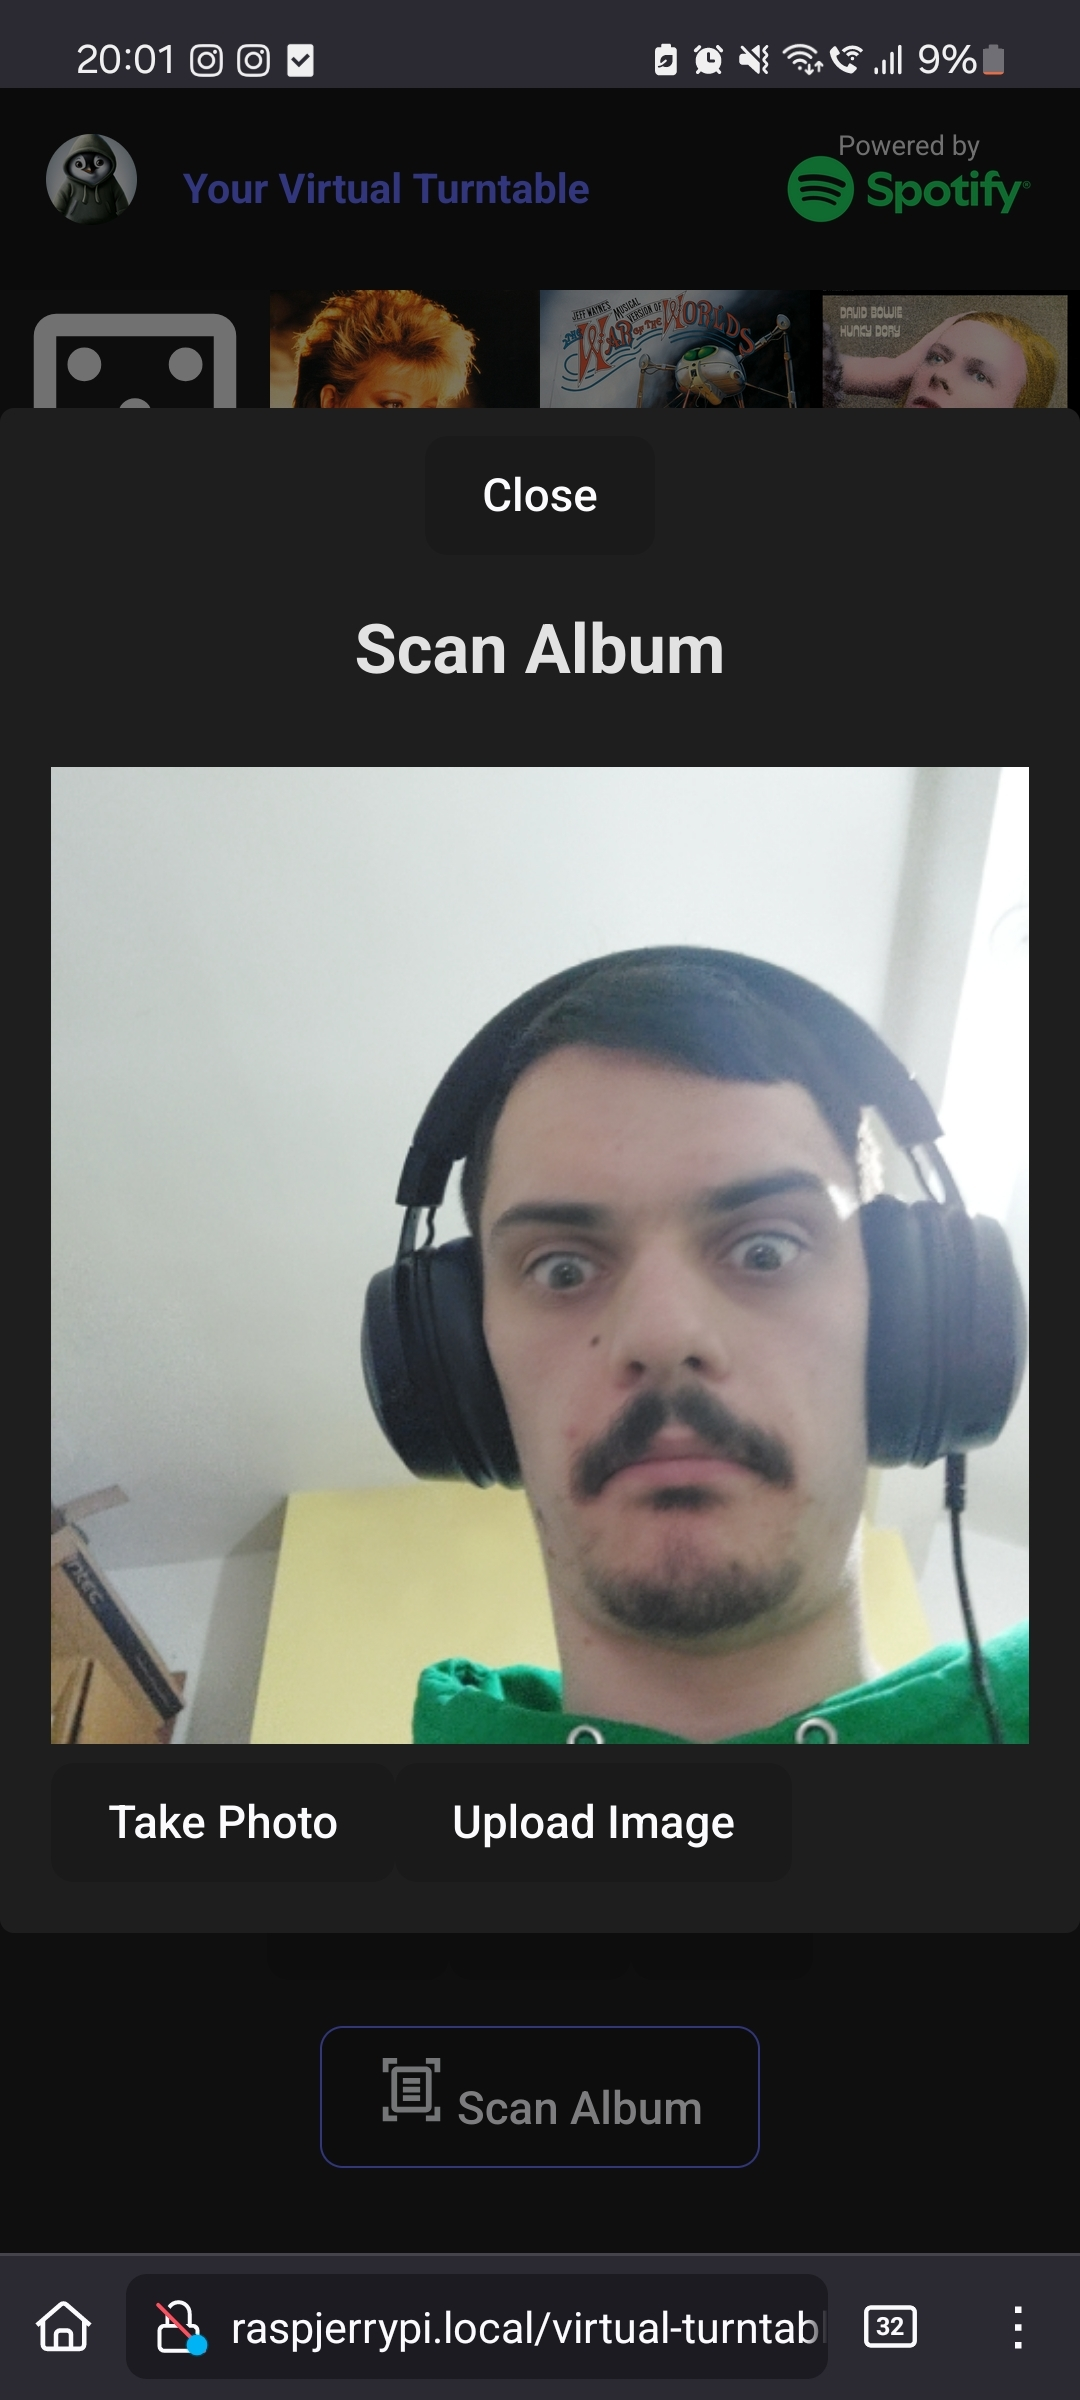
\includegraphics[width=\textwidth]{images/screenshots/PHONE_Cam.jpg}
                    \caption{Screenshot of a remote client (mobile) using the camera functionality}
                    \label{fig:phoneCam}
                \end{minipage}
                \hfill
                \begin{minipage}[b]{0.45\textwidth}
                    \centering
                    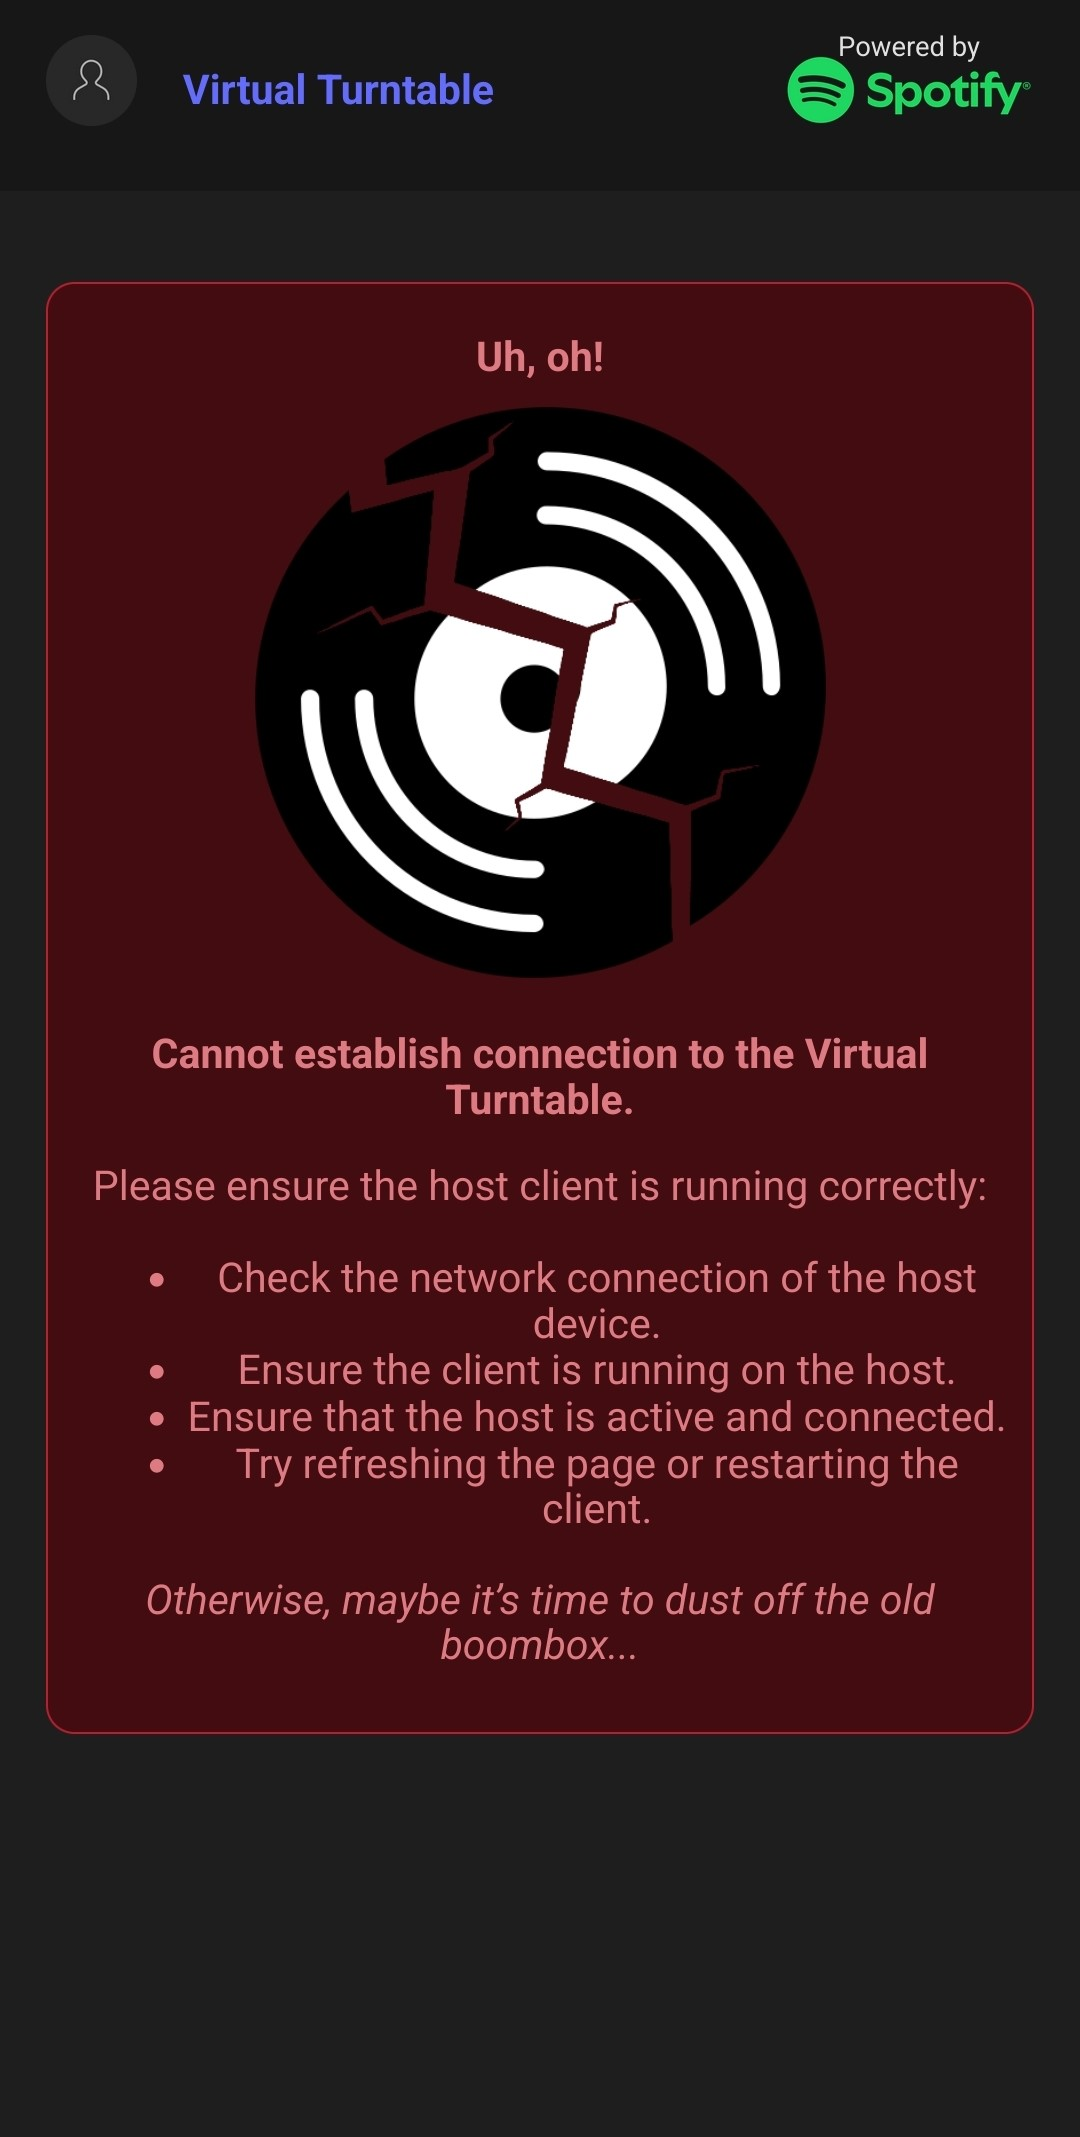
\includegraphics[width=\textwidth]{images/screenshots/PHONE_Error.jpg}
                    \caption{Screenshot of a remote client displaying a 404 error}
                    \label{fig:phoneError}
                \end{minipage}
            \end{figure}
    
        \section{Supplementary Information}
    
            \subsection{Mythological Inspiration} \label{app:Greek}
    
                \paragraph{Ouroboros} A mythological serpent known for circling and eating its own tail, as in Figure~\ref{fig:ouroboros}. This name was used for the simple one-headed CNN model design, which 'self-fed' on deployment data with a low-distribution shift between its training data.
    
                \paragraph{Amphisbaena} A snake-like creature, also of origin in Greek mythology, with a notable second head at the end of its tail, as in Figure~\ref{fig:amphisbaena}. This creature's name was used for the two-headed neural network design.
    
                \paragraph{Hydra} A rather famous mythological Greek monster, the Hydra of Lerna is a serpentine lake monster, famed for having many heads. These carying number of heads are most well-known for the fact that for every one that was cut off, two more would re-grow in its place. This creature's name was used for the PNN model design, which featured a growing number of heads.
    
                \begin{figure}[h]
                    \centering
                    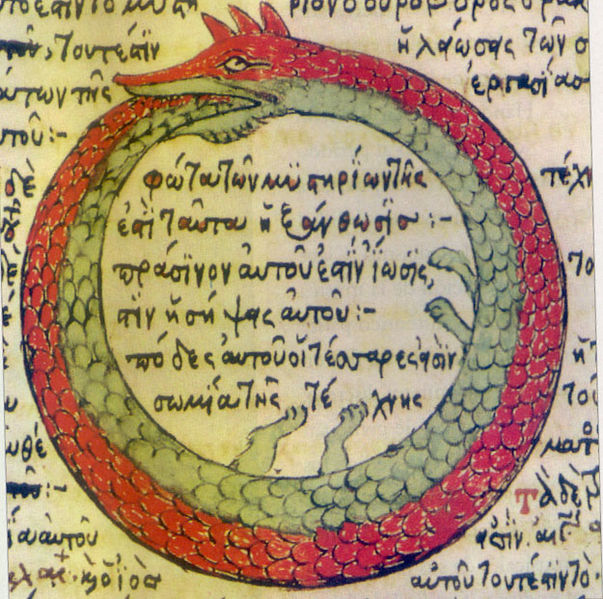
\includegraphics[width=0.6\textwidth]{images/Ouroborus.jpg}
                    \caption{A drawing of an ouroboros, in an alchemical tract (1478)}
                    \label{fig:ouroboros}
                    \caption*{Source: \href{https://en.wikipedia.org/wiki/File:Serpiente_alquimica.jpg}{Wikipedia}}
                \end{figure}
    
                \begin{figure}[h]
                    \centering
                    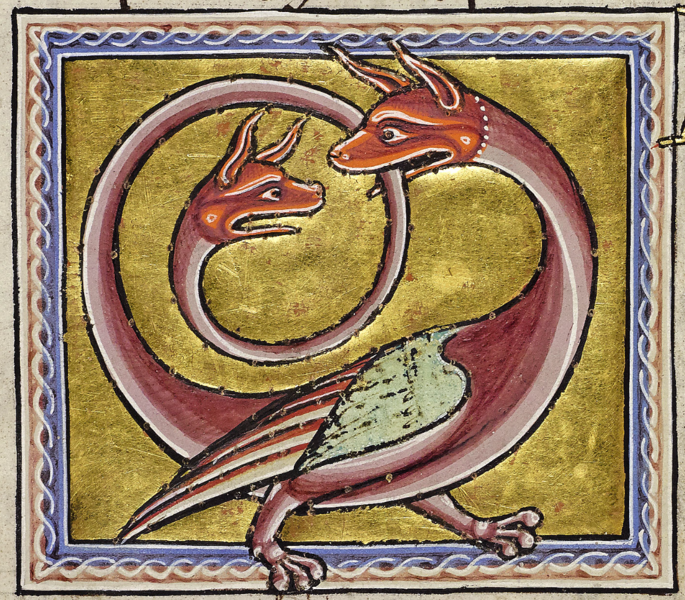
\includegraphics[width=0.6\textwidth]{images/Amphisbaena.png}
                    \caption{An illustration of an amphisbaena (c. 1200)}
                    \label{fig:amphisbaena}
                    \caption*{Source: \href{https://www.abdn.ac.uk/bestiary/ms24/f68v}{The Aberdeen Bestiary, folio 68V.}}
                \end{figure}
    
            \subsection{Cultural Inspiration} \label{app:Cult}
    
                \paragraph{Ed Sheeran Meme} As a light-hearted cultural reference, a meme (Figure~\ref{fig:EdMeme}) highlighting the uniformity of Ed Sheeran’s album art served partially as inspiration for designing a artist classifier. The visual similarity in album covers suggested that artist and album may be decoupled yet jointly learnable.
    
                \begin{figure}[H]
                    \centering
                    
\includegraphics[width=0.6\textwidth]{images/EdSheeranMeme.jpg}
                    \caption{A social media post jokingly referencing the consistent visual theme of Ed Sheeran's album covers}
                    \label{fig:EdMeme}
                    \caption*{Source: \href{https://www.threads.net/@pun_bible/post/DB83pw3gZSh/media}{\@pun\_bible (threads.net)}}
                \end{figure}
    
        \section{Ponderings on what the project expresses} \label{sec:nailArt}
    
        At the centre of this system lies a single vinyl disc (see \ref{fig:product}), fixed in place. It serves no functional role in audio playback, but instead acts as a blank canvas — spinning beneath a projector that overlays metadata and centre-label imagery. The user’s actual records are never played, only scanned via their sleeves, preserving them entirely. This one disc, however, is not so fortunate.
    
        A nail, mounted in place of a stylus, crudely scratches against the rotating surface. Though mechanically redundant, it produces a faint scraping sound -- evoking the familiar hiss of analogue playback. Ironically, this unintended acoustic artefact became central to the experience: an authentic, physical sound that reinforces the illusion of vinyl, even as the music itself is streamed digitally. Yet the sound emitted is, in fact, the destruction of the vinyl’s own grooves -- the very data it once held, gradually scraped away.
        
        What began as a visual flourish now feels almost symbolic. The system preserves physical media, yet requires one record to be worn down in the process. A vinyl that exists purely to look like any vinyl, its own centre label concealed beneath a blank white sheet to be projected upon in mimicry; and to sound like a generic vinyl — forced to scrape and screech, but not its own original composition, which is instead destroyed with each rotation. In retrospect, it's a strange reversal: a digital player that needs physical damage to feel more analogue. A disc slowly degrading under a metal point to lend authenticity to a digital experience.
        
        None of the user’s own records are harmed, yet this one sacrificial vinyl remains essential. It makes no contribution to the music, yet is critical to the illusion. It is not played, but must still be heard -- not for the value of what it once held, but for what it now represents.
        
        There is something both comical and oddly poetic in this inversion: a system that digitises collections, yet requires a physical artefact to feel analogue. In hindsight, this unintentional arrangement reflects a curious tension -- between preservation and performance, where simulation relies on the very thing it seeks to replace.
        
        %\section{Other appendices as necessary}
    \end{uomappendix}
    
    
    %%%%%%%%%%%%%%%%%% END MATTER %%%%%%%%%%%%%%%%%%
    %TC:endignore
    \end{document}